\section{Opportunités}\label{sec:oppo}
%%%%%%%%%%%%%%%%%%%%%%%%%%%%%%%%%%%%%%%%%%%%%%%%%%%%%%%%%%%%%%%%%%%%%%%%
    
    %Fin d'un modèle
    Nous avons montré dans les sections précédentes que de poursuivre la stratégie qui consistait à ajouter toujours plus de serveurs pour construire un supercalculateur, n'est plus viable. Nous avons présenté les principaux challenges que les utilisateurs de HPC doivent relever et les barrières rencontrées. Pour y parvenir, des évolutions technologiques majeures doivent être faites ainsi que de repenser l'architecture des plateformes.
    Ce constat est partagé par le rapport de Pathforward \cite{Lucas2014}: ``\textit{Les améliorations considérables nécessaires à la réalisation d'un supercalculateur \gls{exascale} ne seront pas satisfaites par des améliorations progressives des techniques conventionnelles actuelles.}''
    Si les challenges sont nombreux et difficiles à relever, de nombreuses opportunités sont disponibles. Dans cette section, nous présentons les opportunités principales à considérer: l'apparition de nouvelles technologies très différentes de celles actuellement utilisées et la reconsidération complète de l'architecture des plateformes. 


\subsection{Investissements financiers}
%%%%%%%%%%%%%%%%%%%%%%%%%%%%%%%%%%%%%%%%%%%%%

    La première condition pour réaliser les nombreux développements technologiques nécessaires est la présence d'investissements financiers. L'industrie du HPC investit massivement dans le développement de nouvelles technologies pour répondre au besoin de puissances de calculs. Une analyse de marché paru en 2016 montre que le marché du High Performance Computing pèsera 36 milliards de dollars en 2020, alors qu'il en valait 28 en 2015\footnote{\url{http://www.marketsandmarkets.com/Market-Reports/Quantum-High-Performance-Computing-Market-631.html}}.

    Si le développement des plateformes exascales est motivé par son aspect financier pour les industries, la construction du premier supercalculateur exascale est un enjeu politique pour les nations. Comme le fut autrefois la conquête lunaire, les nations ont à coeur d’être les premières à obtenir une telle architecture et s’en donnent les moyens. L’obtention d’une telle performance est un symbole qui mettra en lumière les acteurs qui y parviendront en premier (nations, universités, constructeurs).

    \paragraph{Investissements Européens} Dans le classement du TOP500 paru en novembre 2017, aucun des 10 supercalculateurs les plus puissants et seulement 5 des 20 meilleurs supercalculateurs mondiaux sont installés en Europe. Alors que l'Asie et l'Amérique se partagent près de 80\% de la puissance de calcul mondiale, l’Europe n'en possède que  18.8\% sur son territoire (voir \autoref{fig:edl_top500_continent}).
    
    \begin{figure}
        \center
        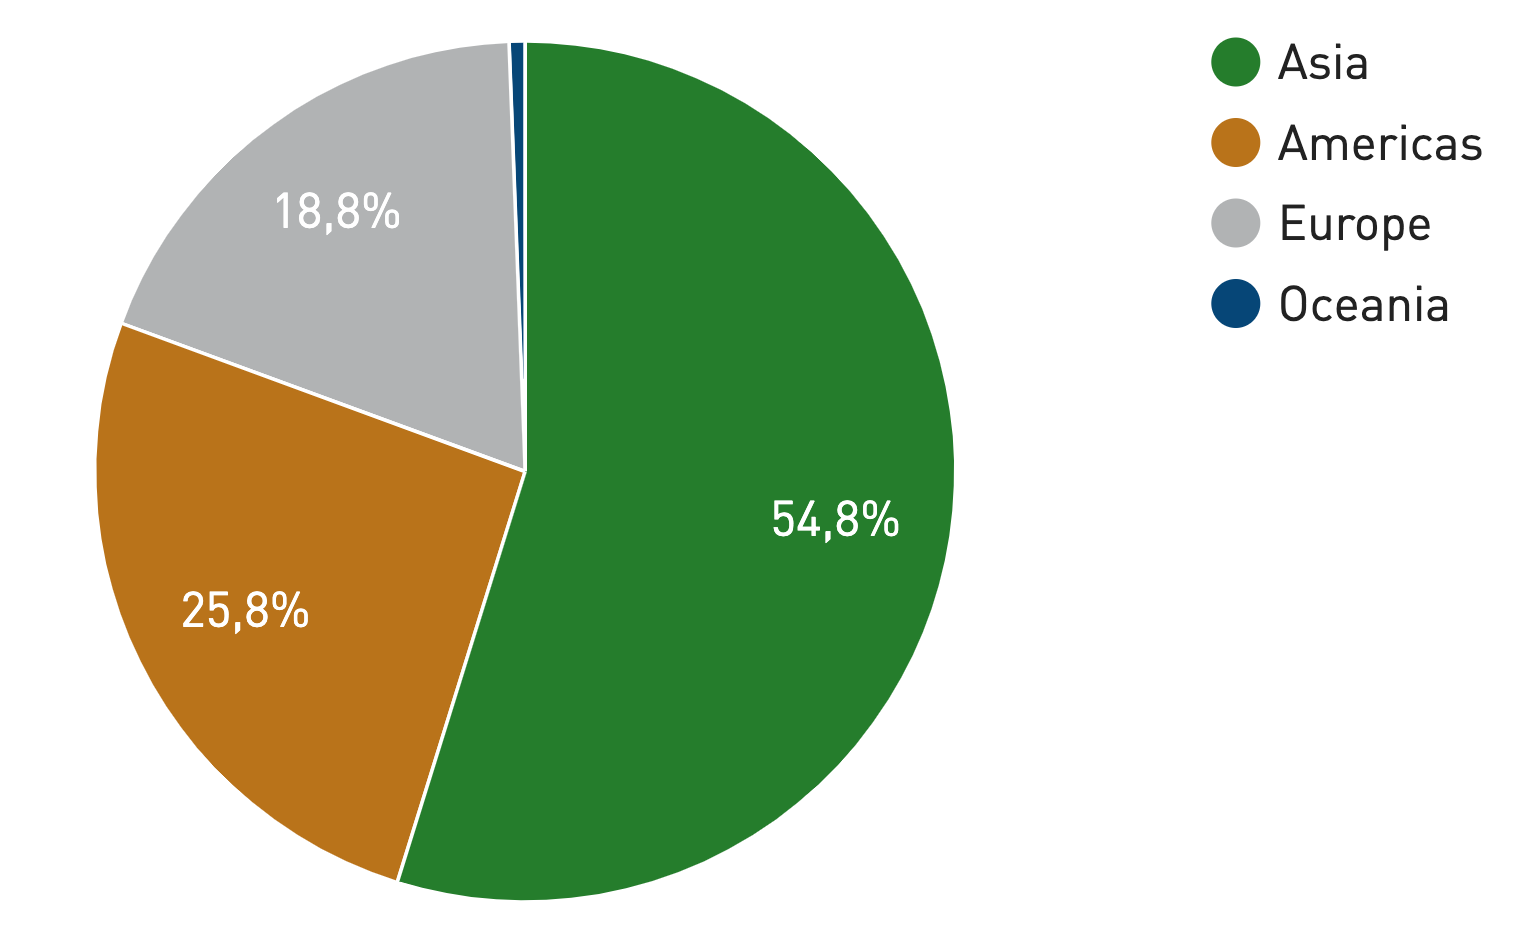
\includegraphics[width=10cm]{images/edl_top500_continent.png}
        \caption{\label{fig:edl_top500_continent} Répartition de la puissance de calcul du Top500 de novembre 2019 entre les continents.}
    \end{figure}
    
    
    Pour accélérer le développement de ses infrastructures, l’Europe a financé un grand projet nommé Horizon 2020. Horizon 2020 est le plus grand programme de recherche et d'innovation jamais mis en place par l'Union européenne. Ce projet d’envergure prévoit d’investir 79 milliards d’euros de 2014 à 2020 pour développer trois piliers : l'excellence scientifique, la primauté industrielle et les défis sociétaux.
    En janvier 2018, la Commission européenne a annoncé investir 1 milliard dans un partenariat réalisé entre le domaine public et privé nommé EuroHPC \cite{EuroHPC2018}. Les objectifs d'EuroHPC sont de développer et déployer une infrastructure de calcul de classe mondiale. 
    Cette entreprise communautaire aura pour objectif de construire 6 supercalculateurs: 2 supercalculateurs petascale ($10^{16}$ opérations) et deux infrastructures ``\textit{pré exascale}'' en 2021. Les architectures pré exascale vont permettre d'utiliser les premières versions des processeurs développées par EuroHPC. Pour assurer son indépendance technologique, le projet EPI (\textit{European Processor Initiative}) a pour objectif de développer de nouveaux processeurs et des accélérateurs MPPA (\textit{massively parallel processor array}) produits par Kalray à Grenoble (voir \autoref{fig:edl_epi_processor}). Enfin, le supercalculateur exaflopique européen prévu entre 2022 et 2023 pourra compter sur des nouvelles architectures, très efficaces énergétiquement, basées sur des processeurs ARM actuellement en développement. Une des motivations étant de réduire sa dépendance aux autres pays pour être plus compétitif.  

    \begin{figure}
        \center
        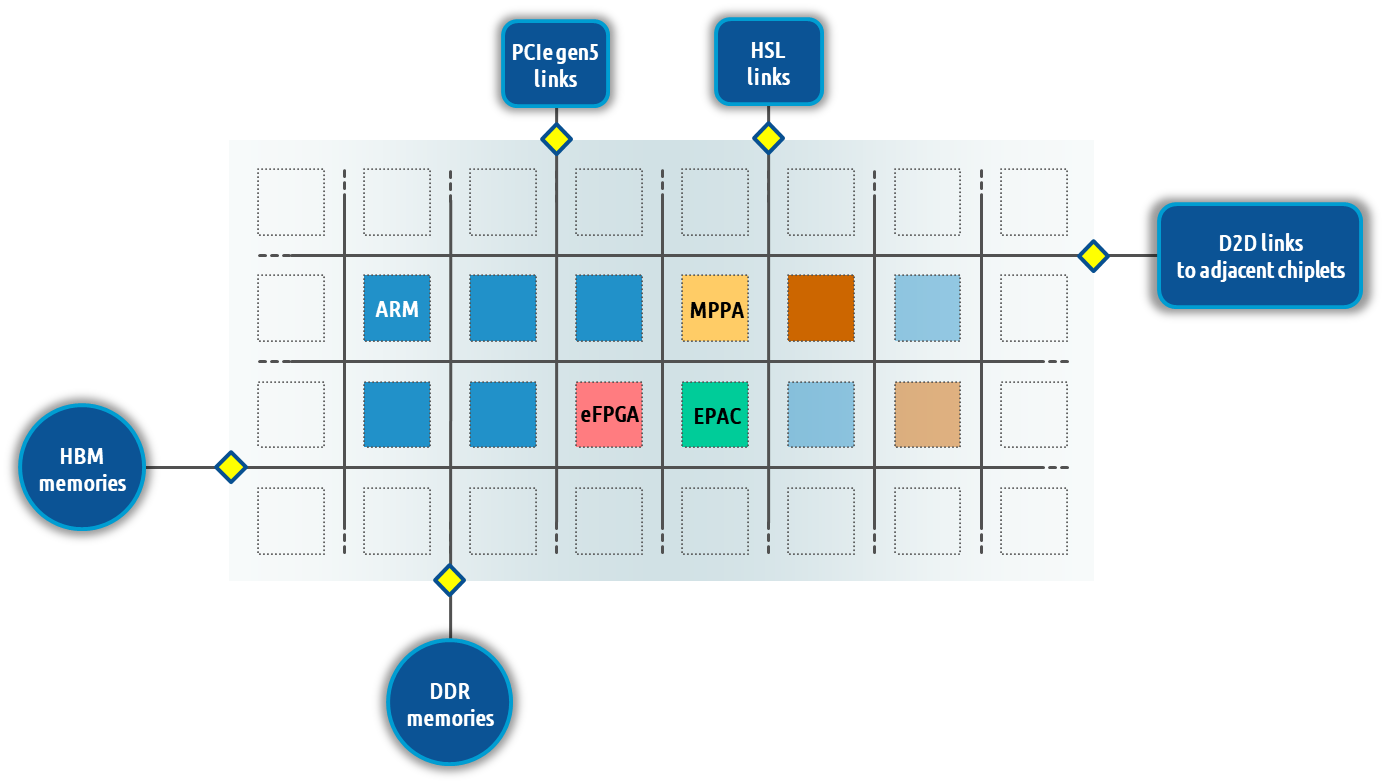
\includegraphics[width=14cm]{images/edl_epi_processor.png}
        \caption{\label{fig:edl_epi_processor} Processeurs GPP utiliseront un réseau à mailles 2D sur la puce permettant de relier différents types de coeurs: ARM-V, FPGA embarqué (eFPGA) pouvant être reprogrammé, un processeur vectoriel (MPPA).}
    \end{figure}
    
    
    \paragraph{Les États-Unis.}
    En 2017, le département des énergies américain a annoncé le financement d'un projet de 232 millions d'euros nommé PathForward. Ce budget est réparti entre 6 entreprises américaines (HPE, AMD, Cray, IBM, Intel et Nvidia) qui doivent ajouter 40\% de financement supplémentaire pour un total de plus de 400 millions d'euros. L'objectif de ce projet est de construire le premier ordinateur \gls{exascale} en 2021 en finançant les développements matériels et logiciels nécessaires.


        
    %%%%%%%%%%%%%%%%%%%%%%%%%%%%%%%%%%%%%%%%%%%


\subsection{Nouvelles technologies mémoires.}\label{sec:oppo_new_memory}
%%%%%%%%%%%%%%%%%%%%%%%%%%%%%%%%%%%%%%%%%%%%%%%%%%        

    %HISTORIQUE: evo + memory Gap 
    \subsubsection{Le trou de la mémoire}
    
        L'évolution des capacités opérationnelles des processeurs et de la performance des mémoires (débits, latence, taille) a été très inégale. La \autoref{fig:edl_memory_pyramide} présente sous forme de pyramide les différentes technologies mémoires actuellement utilisées dans le système. Les trois principaux facteurs les différenciant les différentes technologies mémoires sont: le prix, la latence d'accès et la capacité (densité). Pour mieux appréhender la différence de latence des technologies, nous les convertissons dans un temps plus facilement appréciable pour un humain. Si un accès au cache L1 prenait 3 secondes, un accès mémoire prendrait alors plus de 5 minutes. Si la donnée à accéder se trouve sur un disque SSD, il faudrait attendre 3 heures avant de la recevoir. Si celle-ci se trouve sur un disque optique, il faudrait alors patienter 10 mois. Il est facile de comprendre pourquoi le \textit{manque} (\textit{miss}) d'une donnée dans le cache pénalise énormément la performance d'une application. 
        
        \begin{figure}
            \center
            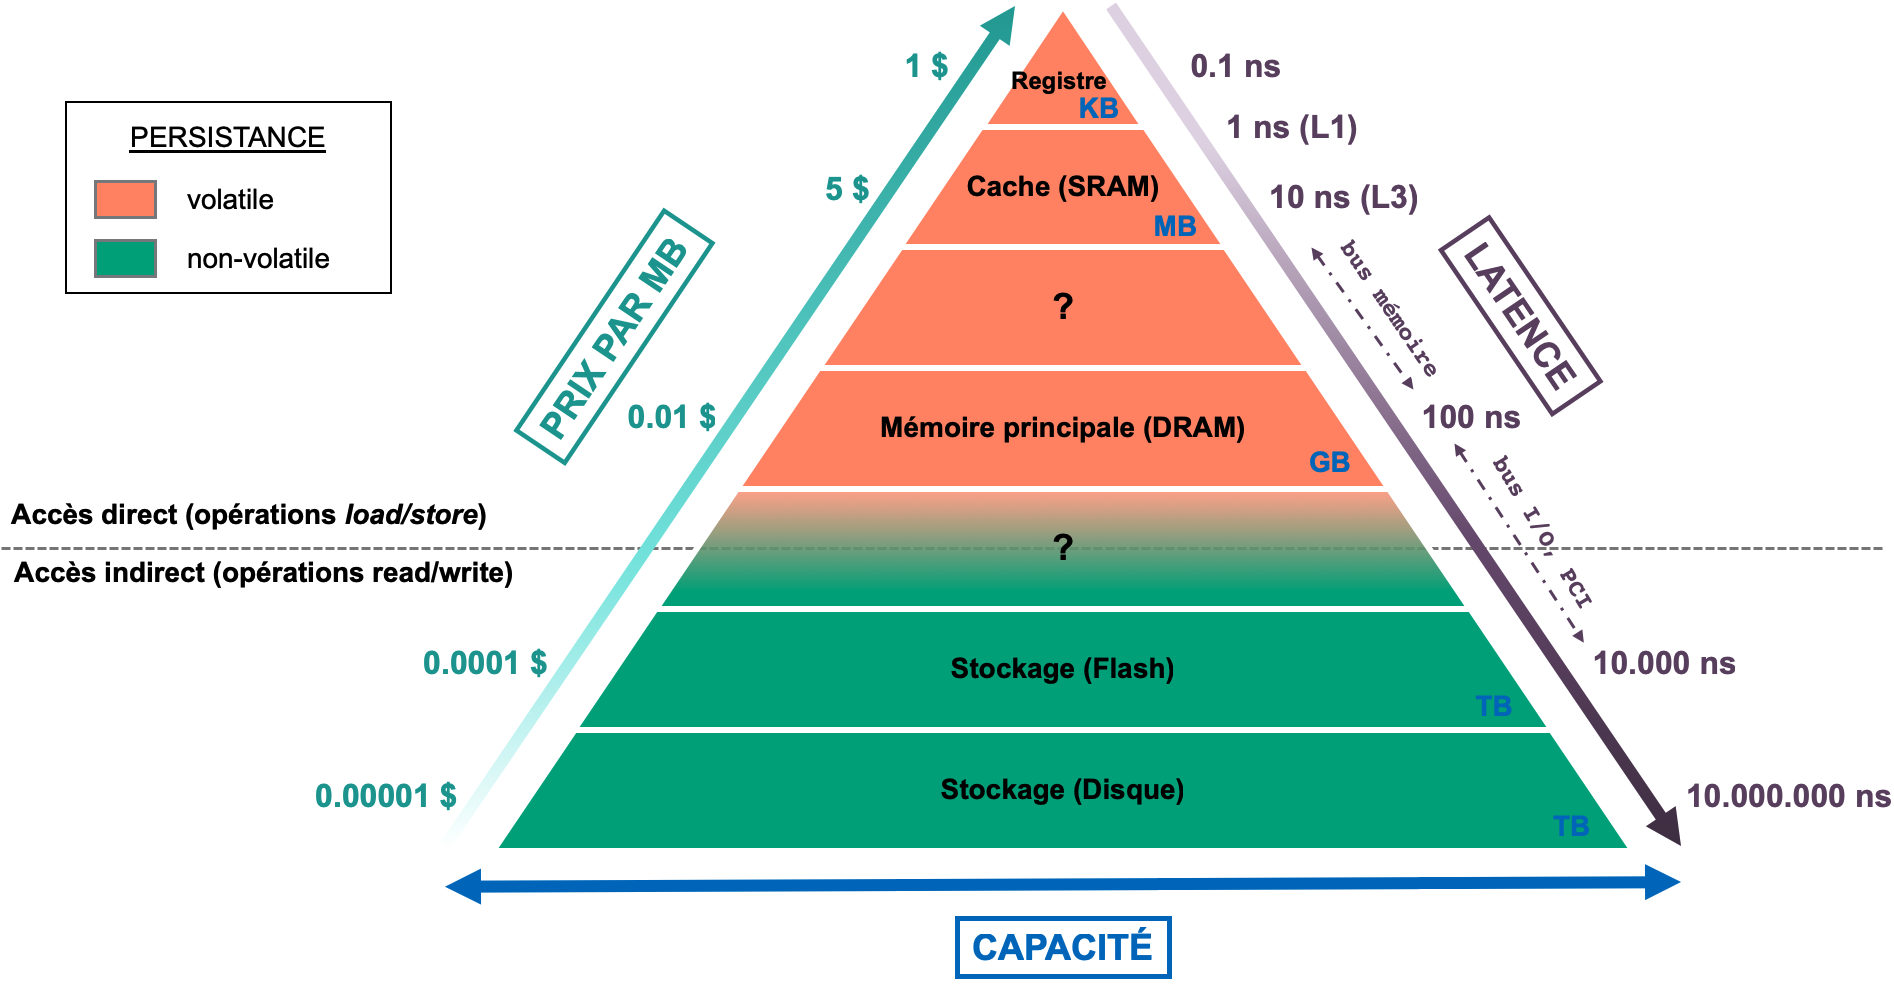
\includegraphics[width=17cm]{images/edl_memory_pyramide.png}
            \caption{\label{fig:edl_memory_pyramide} Hiérarchisation des différents types de mémoire en fonction du coût, de la latence et de la capacité de stockage habituellement utilisé dans les architectures.}
        \end{figure}
        
        Malgré le développement d'une hiérarchie mémoire (voir \autoref{sec:hierarchie}) pour réduire ces écarts de performance, nous remarquons  la présence de deux \textit{trous} (\textit{memory gap}) de performance. Pour résoudre ce challenge, l'industrie poursuit le travail débuté avec l'introduction de la hiérarchie mémoire grâce à deux solutions: 
        \begin{itemize}
            \item Réaliser le traitement directement dans la mémoire grâce aux techniques de calculs en mémoire (\textit{processing-in memory} (PIM)) \cite{Singh2019}. En déplaçant le calcul en mémoire, les latences d'accès sont réduites et les débits augmentés. Des implémentations d'architecture PIM utilisent des mémoires SRAM qui ont permis d'accélérer des algorithmes d'apprentissage machine \cite{Zhang2016, Biswas2018, Kang2018}. D'autres implémentations utilisent de la mémoire DRAM \cite{Seshadri2017} \cite{Li2017} permettant de réaliser des opérations logiques \verb|AND| et \verb|OR| sur des  barrettes mémoires DRAM classique non modifiée \cite{Gao2019}. Des technologies comme le memristor permettent de réaliser des multiplications de matrices dont chaque valeur peut être calculée simultanément. Ce composant électronique a été décrit par Leon Chua en 1971 dans l'article ``\textit{ Memristor - The Missing Circuit Element}''  \cite{Chua1971}. La première implémentation physique a été réalisée par une équipe de recherche des laboratoires d'HP conduite par Stanley Williams en 2008 et publiée dans l'article ``\textit{The missing memristor found}'' \cite{Strukov2008}. Cette mémoire permet d'encoder un nombre réel sur un seul bit. L'information encodée peut ainsi avoir une infinité de valeurs contrairement à deux valeurs pour les bits des mémoires utilisées habituellement.
            
            \item La deuxième solution permettant d'accélérer les accès mémoire est de combler les deux \textit{trous} de performance constatés sur la \autoref{fig:edl_memory_pyramide} grâce au développement de nouvelles technologies mémoires. Les différentes solutions envisagées sont discutées dans le reste de cette section.
        \end{itemize}
        
        
    
    
    \subsubsection{Trou entre SRAM et DRAM} 
        Pour réduire le trou séparant les mémoires caches et la mémoire centrale, les processeurs ont vu leur dernier niveau de cache s'agrandir. Cependant, la mémoire SRAM utilisée est très chère à produire et sa densité ne permet plus de les agrandir. Côté mémoire principale, le développement de différentes technologies mémoires (DDR3, DDR4, DDR5) ne permet pas de faire évoluer fortement la performance des applications. La raison principale vient de la difficulté à augmenter le débit du bus mémoire qui est limité par le nombre de broches utilisables sur le processeur. La \autoref{fig:edl_channel_pin} montre l'évolution de la proportion de broches d'un processeur qui est affectée au bus mémoire. Il est aujourd'hui très difficile d'allouer plus de broches pour le bus mémoire. Le nombre de canaux a augmenté, permettant d'améliorer le débit du bus mémoire. Cependant, le nombre de coeurs a lui aussi évolué, bien plus rapidement que le nombre de canaux mémoires. Ainsi, la bande passante mémoire par coeur est passée de 6.4 Gb/s pour un processeur de 8 coeurs en 2012 à 4.6 Gb/s pour un processeur de 28 coeurs en 2016. 
        
        \begin{figure}
            \center
            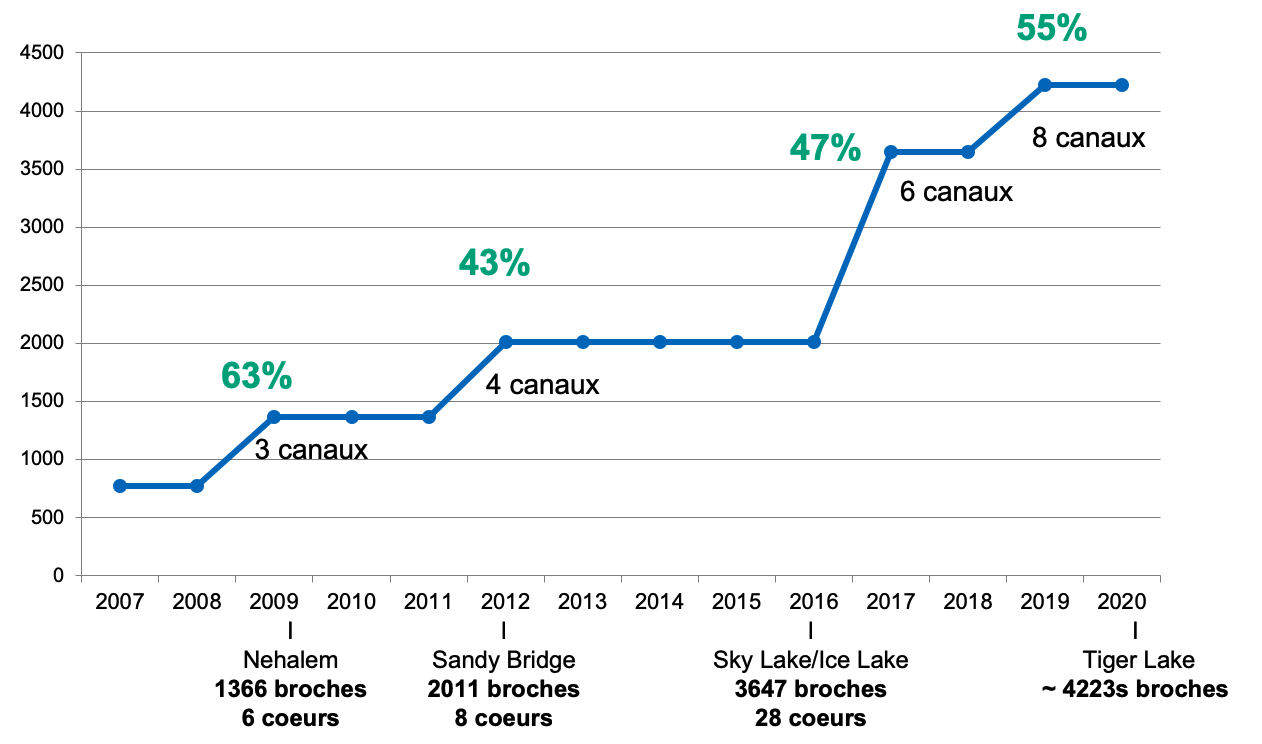
\includegraphics[width=12cm]{images/edl_channel_pin.png}
            \caption{\label{fig:edl_channel_pin} Nombre et proportion de broches allouée aux bus mémoires des dernières architectures de processeur Intel.}
        \end{figure}
    
    
        À partir de ce constat, et celui fait dans la \autoref{sec:edl_chal_energie} concernant la consommation énergétique du système mémoire, les architectures ont été repensées pour placer la mémoire directement sur les puces (\textit{On Package Memory}) au plus proche des circuits de traitement (\textit{near-memory processing}). En plaçant la mémoire directement sur la puce du processeur, les limitations imposées par le bus mémoire (débit, consommation électrique) peuvent être contournées notamment grâce à l'utilisation de bus plus large (voir \autoref{fig:edl_hbm_vs_gddr5}). Afin de pouvoir installer des espaces mémoire suffisamment larges directement sur la puce nouveau type de mémoire a été développé: les mémoires 3D. La principale différence avec la mémoire conventionnelle est son architecture qui est en 3D. Alors que la mémoire DRAM s’étale sur deux dimensions X, Y, la mémoire 3D s’étend en plus sur une troisième dimension Z en s’empilant (\textit{stack}, voir \autoref{fig:edl_hbm_precis}). En empilant des couches de silicone, ces mémoires sont très denses. Ainsi, 1GB de GGDR5 qui nécessite $672 mm^2$, n'a besoin que de $35 mm^2$ pour la même capacité de mémoire 3D, soit une réduction de 94\%\footnotetext{Mesure réalisée par AMD sur 1GB GDDR5 (4x256MB ICs) et 1GB HBM-2 (1x4-Hi)}. 
        
                   
        
        \begin{figure}[t!]
            \centering
            \begin{subfigure}[t]{0.48\textwidth}
                \centering
                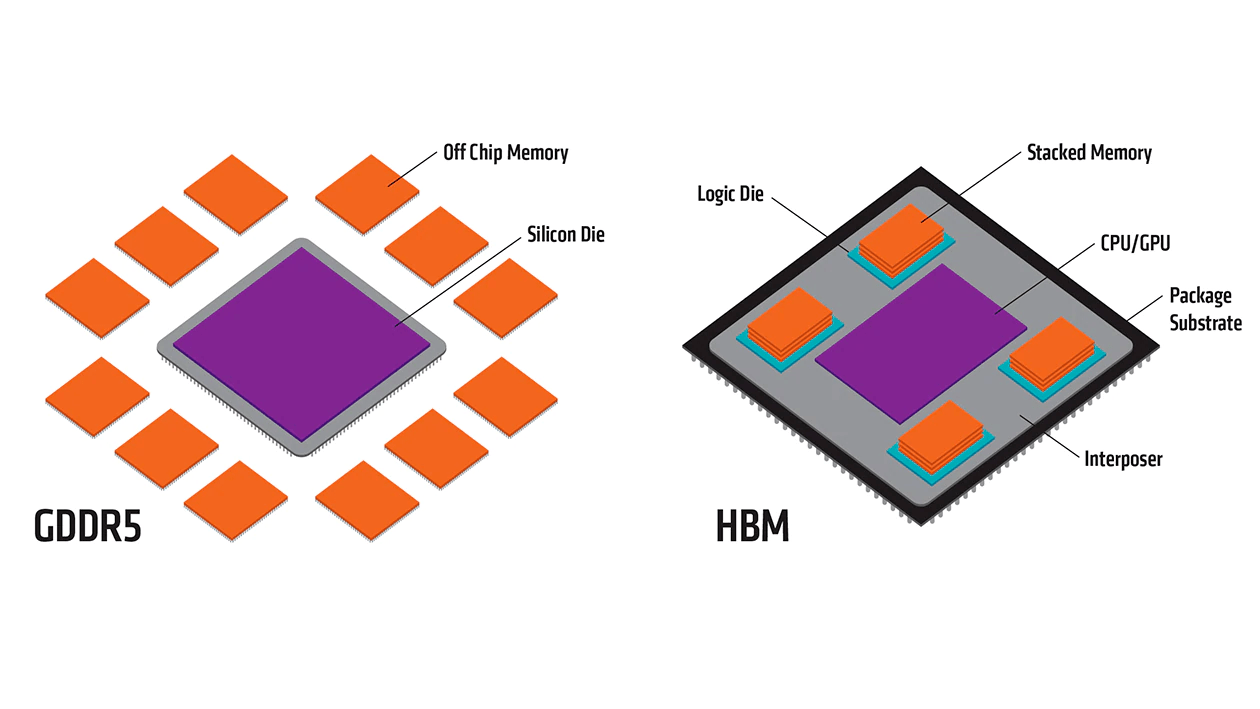
\includegraphics[width=\linewidth]{images/edl_hbm_vs_gddr5.png}
                \caption{\label{fig:edl_hbm_vs_gddr5} Pour atteindre de meilleure performance, les mémoires 3D sont placées directement sur la puce.}
            \end{subfigure}\hfill
            \begin{subfigure}[t]{0.48\textwidth}
                \centering
                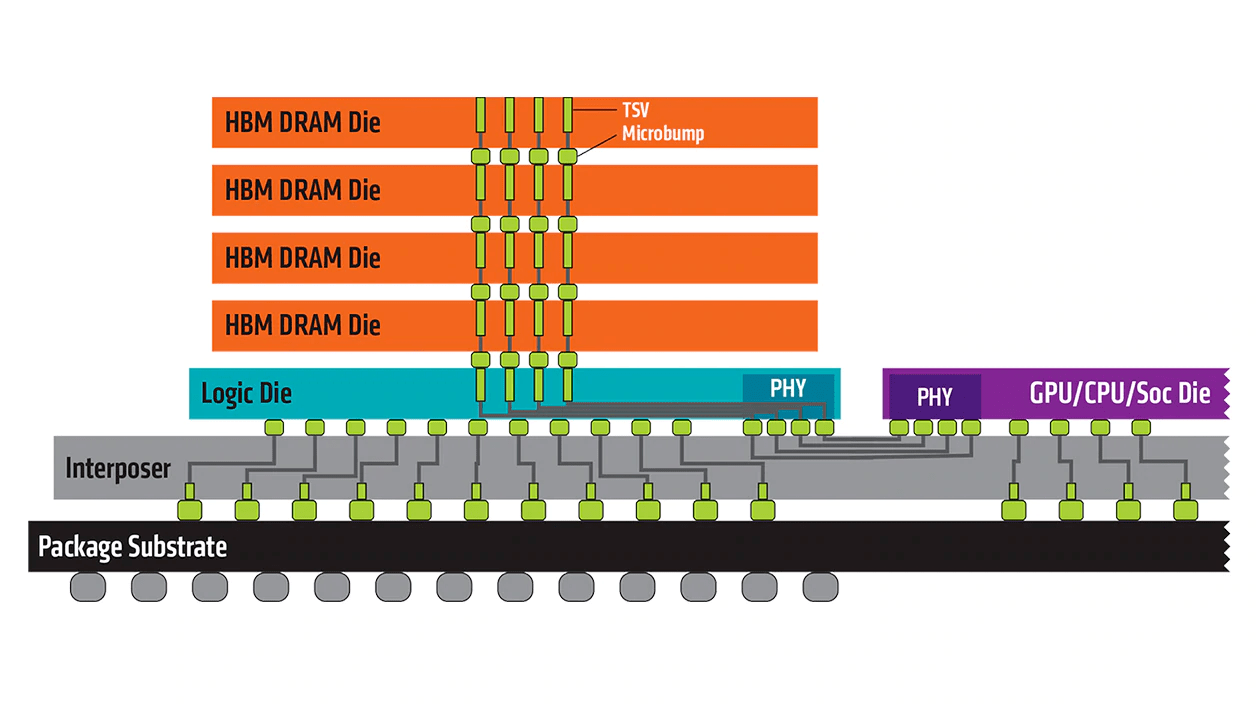
\includegraphics[width=\linewidth]{images/edl_hbm.png}
                \caption{\label{fig:edl_hbm_precis} Les mémoires 3D sont un empilement de mémoire DDR relié à un interposeur grâce à des \textit{vias} (TSV, TCI).}
            \end{subfigure}
            \caption{\label{fig:edl_hbm}Architecture et utilisation d'une mémoire 3D sur un GPU\protect\footnotemark}
        \end{figure}
        \footnotetext{Source AMD - \url{https://www.amd.com/fr/technologies/hbm}}
        
        
        Actuellement, les mémoires 3D sont principalement commercialisés sous les technologies HBM (\textit{High Memory Bandwidth} \cite{Standard2013}) produite par AMD, Samsung et Hynix et de la HMC (\textit{Hybrid Memory Cube}\cite{Jeddeloh2012}) produite par Micron. Les mémoires HBM se composent actuellement de quatre puces DRAM sur une puce de base et possède deux canaux de 128 bits par puce DRAM, soit 8 canaux au total, ce qui donne 1024 bits par pile d'interfaces mémoire (voir \autoref{tab:hmb2_vs_grrd5}). Une carte graphique possédant 4 piles possède ainsi un bus mémoire de 4096 bits. Pour améliorer l'efficacité énergétique, la fréquence des mémoires 3D est moins rapide que celle des mémoires DRAM conventionnelles. De plus la proximité de ces mémoires dites \textit{on-package}, permet de réduire la distance de communication avec les processeurs et de réduire la consommation électrique (3.9 pj/bit pour la HBM2 contre 14 pj/bit pour la GDDR5). Malgré une fréquence plus faible, le large bus mémoire directement connecté à la puce permet d'atteindre des bandes passantes plus élevées. Pour une enveloppe énergétique de 60W, une mémoire GDDR5 est capable de fournir un débit de 536 Gb/s quand une mémoire HBM2 peut atteindre 1.9 Tb/s \cite{OConnor2017}. Les mesures de performances réalisées à l'aide du benchmark Stream ont permis de mesurer des écarts de performances d'un facteur 4 avec une mémoire DDR4 classique\cite{7965110}, tout en consommant 50\% moins d'énergie\footnotetext{Information NVIDIA - \url{https://www.extremetech.com/extreme/226240-sk-hynix-highlights-the-huge-size-advantage-of-hbm-over-gddr5-memory}}. Cependant, des latences d'accès réduites (15\%) ont été mesurées et peuvent impacter la performance de certaines applications. L'utilisation de nombreux coeurs et ainsi que d'instructions de préchargement mémoire peuvent cependant permettre d'atteindre de meilleurs résultats \cite{7965110}.
        
        % Please add the following required packages to your document preamble:
        % \usepackage{graphicx}
        \begin{table}[]
        \centering
        \resizebox{\textwidth}{!}{%
        \begin{tabular}{|l|c|c|c|c|c|c|}
        \hline
        & \textbf{Largeur bus} & \textbf{Capacité (GB)} & \textbf{Débit (Gb/s)} & \textbf{Fréquence mémoire} & \textbf{Bande passante (Gb/s)} & \textbf{Consommation (pj/bit)} \\ \hline
        \textbf{GDDR5} & 768 & 24 & 8 & 1.25 GHz & 480 & 14 \\ \hline
        \textbf{HBM2} & 4096 & 8 & 2 & 1 GHz & 1024 & 4 \\ \hline
        \end{tabular}%
        }
        \caption{Comparaison des mémoires GDDR5 utilisées sur les GPU NVidia K80 et des mémoires HBM2 utilisées sur un GPU utilisant 4 piles de mémoire.}
        \label{tab:hmb2_vs_grrd5}
        \end{table}
         
    \subsubsection{Trou entre DRAM et Flash}
    %%%%%%%%%%%%%%%%%%%%%%%%%%%%%%%%%%%%%%%

        %INTRO
        La nécessité d'augmenter les capacités de stockage, la pression énergétique et la faiblesse d'évolution des performances du système mémoire sont à l'origine du développement de nouvelles technologies visant à combler le trou situé entre la mémoire et le stockage. L'utilisation de ces nouvelles mémoires n'est pas seulement une évolution de performance. Elles vont aussi permettre de développer de nouvelles approches logicielles. Par exemple, lors de l'arrêt d'un ordinateur, si la totalité de la mémoire y est sauvée, le temps de redémarrage sera accéléré. Les applications telles que les bases de données relationnelles qui sont développées pour anticiper les longues latences des disques pour être stockées directement en mémoire sans risque de pertes d'informations (\textit{In memory database} \cite{Oukid2015}). Les applications de simulations numériques pourront rapidement générer des points de contrôle (\textit{checkpoint}), permettant de reprendre le traitement suite à une erreur. 
        
        %En plus des performances, plusieurs spécificités séparent la mémoire principale du stockage:
        %\begin{itemize}
         %   \item L'adressabilité: En mémoire, chaque octet est adressable alors que les disques sont adressés par blocs de plusieurs octets (généralement 512 octets).
          %  \item Les opérations: En mémoire le processeur peut directement travailler sur les données grâce aux opérations \textit{load/store}. Le stockage est lui géré par des opérations d'entrée/sortie telles que \textit{read/write}.
           % \item La persistance: lorsque le courant est coupé, les données présentes en mémoire sont effacées contrairement au stockage.
        %\end{itemize}
        
        %Critère
        
        L'objectif est donc de développer de nouvelles mémoires ayant les avantages des deux technologies (DRAM et flash) sans leurs inconvénients. Plusieurs critères sont alors essentiels pour leur adoption (\cite{Freitas2008}). Le premier  concerne la persistance des données, permettant entre autres de réduire leur consommation énergétique. Pour des raisons de fiabilité et de densité, ces mémoires ne doivent pas contenir de partie mobile telles qu'un disque rotatif. Pour être utilisées comme mémoire, ces nouvelles technologies doivent pouvoir atteindre des latences d'accès faibles (autour de 200 ns\cite{IBM2013}), proches de celle de la DRAM. Les technologies développées doivent être endurantes pour pouvoir être utilisées intensivement (entre $10^9$ et $10^{12}$ écritures par cellule \cite{IBM2013}). À terme, ces technologies devraient remplacer les mémoires DRAM, elles doivent donc être adressables par octet. Enfin, pour être accepté par l'industrie, le prix de ces mémoires doit être compétitif avec les technologies existantes. Avec les critères exposés précédemment, nous constatons qu'il n'est pas possible de compter sur les technologies existantes:
        \begin{itemize}
            \item Les disques optiques permettent d'obtenir de grande capacité de stockage. Cependant, à cause des parties mécaniques (disques rotatifs, bras de lecture) les latences et les débits sont trop faibles. De plus, pour obtenir des latences acceptables, les disques doivent tourner continuellement, impactant leur consommation énergétique et leur fiabilité.
            \item La technologie flash ne possède pas une endurance aux écritures suffisante ($10^6$ écritures), loin des objectifs fixés ($10^9$ écritures). De plus, par héritage des disques optiques, les disques SSD ne sont adressables que par bloc.
            \item La mémoire DRAM possède de très bonnes performances en lecture comme en écriture. Cependant, sa densité est faible et elle doit constamment être alimentée pour conserver ses données, impactant la consommation électrique.
        \end{itemize}
        %: la densité, la volatilité et le prix des disques associé à latences et l'endurance de la mémoire. 
  
        
    
        
        %DEFINITION SCM
        \paragraph{NVM, NVRAM ou SCM ?}
            
            De nombreux termes sont utilisés dans la littérature pour les désigner ces nouvelles mémoires: NVM (\textit{non-volatile memory}), NVRAM (\textit{non volatile RAM}) ou encore PM (\textit{persistent memory}). Le terme NVM est souvent confondu avec le terme NVMe qui désigne un nouveau protocole de communication visant à remplacer le protocole SATA. Les différentes implémentations des NVRAM sont présentées sur la \autoref{fig:memoire_stockage_def}. Le premier critère de classement est celui de la volatilité puis de l'adressabilité. La seule NVRAM couramment utilisée qui n'est adressable qu'en bloc est la mémoire flash, ne répondant ainsi pas au critère d'adressabilité fixé ci-dessus. Il y a ensuite deux façons d'implémenter des NVRAM adressables par octet qui sont présentées dans la suite de cette section:
            \begin{itemize}
                \item Les NVDIMM (non volatile DIMM) 
                \item Les SCM (\textit{storage class memory})
            \end{itemize}
            
            
            \begin{figure}
                \center
                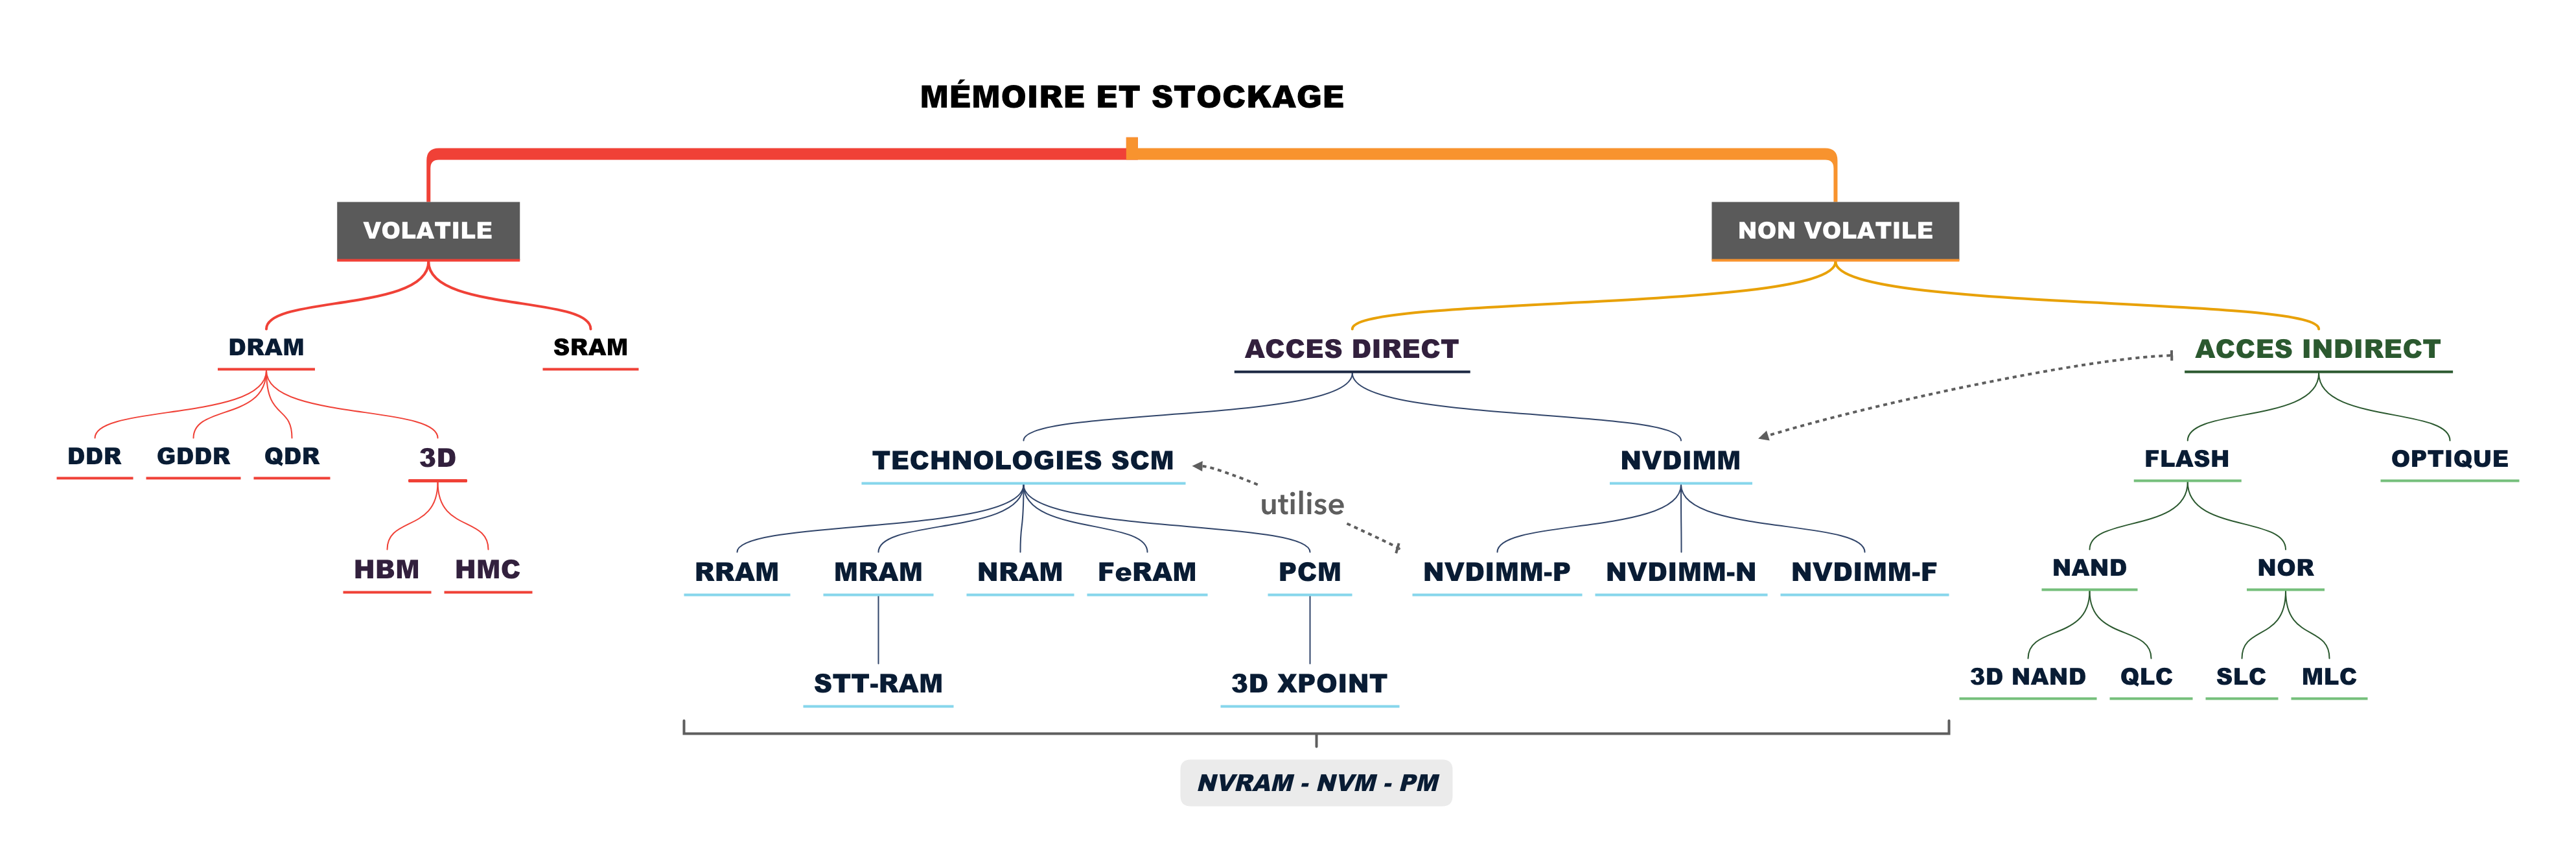
\includegraphics[width=17cm]{images/memoire_stockage_def.png}
                \caption{\label{fig:memoire_stockage_def} Tri des technologies de stockage en fonction de la volatilité et l'adressabilité.}
            \end{figure}
    
    
    %%%%%%%%%%%%%%%%%%%%%%%%%%%%%
    
    \paragraph{Les NVDIMM.}\label{sec:nvdimm}
    
        La NVDIMM est une technologie mémoire qui utilise le même format que les barrettes de mémoires classiques DRAM \cite{ChrisEvans2017}, elle peut donc être adaptée sur les serveurs actuels. Le système d'exploitation doit cependant être adapté pour profiter des avantages de la persistance et être, par exemple, capable de redémarrer directement à partir des données se trouvant en mémoire (les versions supérieures à Linux 4.4 sont compatibles). L'organisation JEDEC\footnote{JEDEC - \url{https://www.jedec.org/}} a été créée en 1958 et développe, entre autres, les standards utilisés en micro électronique. L'organisation a publié 3 standards pour le développement des NVDIMM (voir \autoref{fig:edl_nvdimm}).
    
            \begin{figure}[t!]
                \centering
                \begin{subfigure}[t]{0.50\textwidth}
                    \centering
                    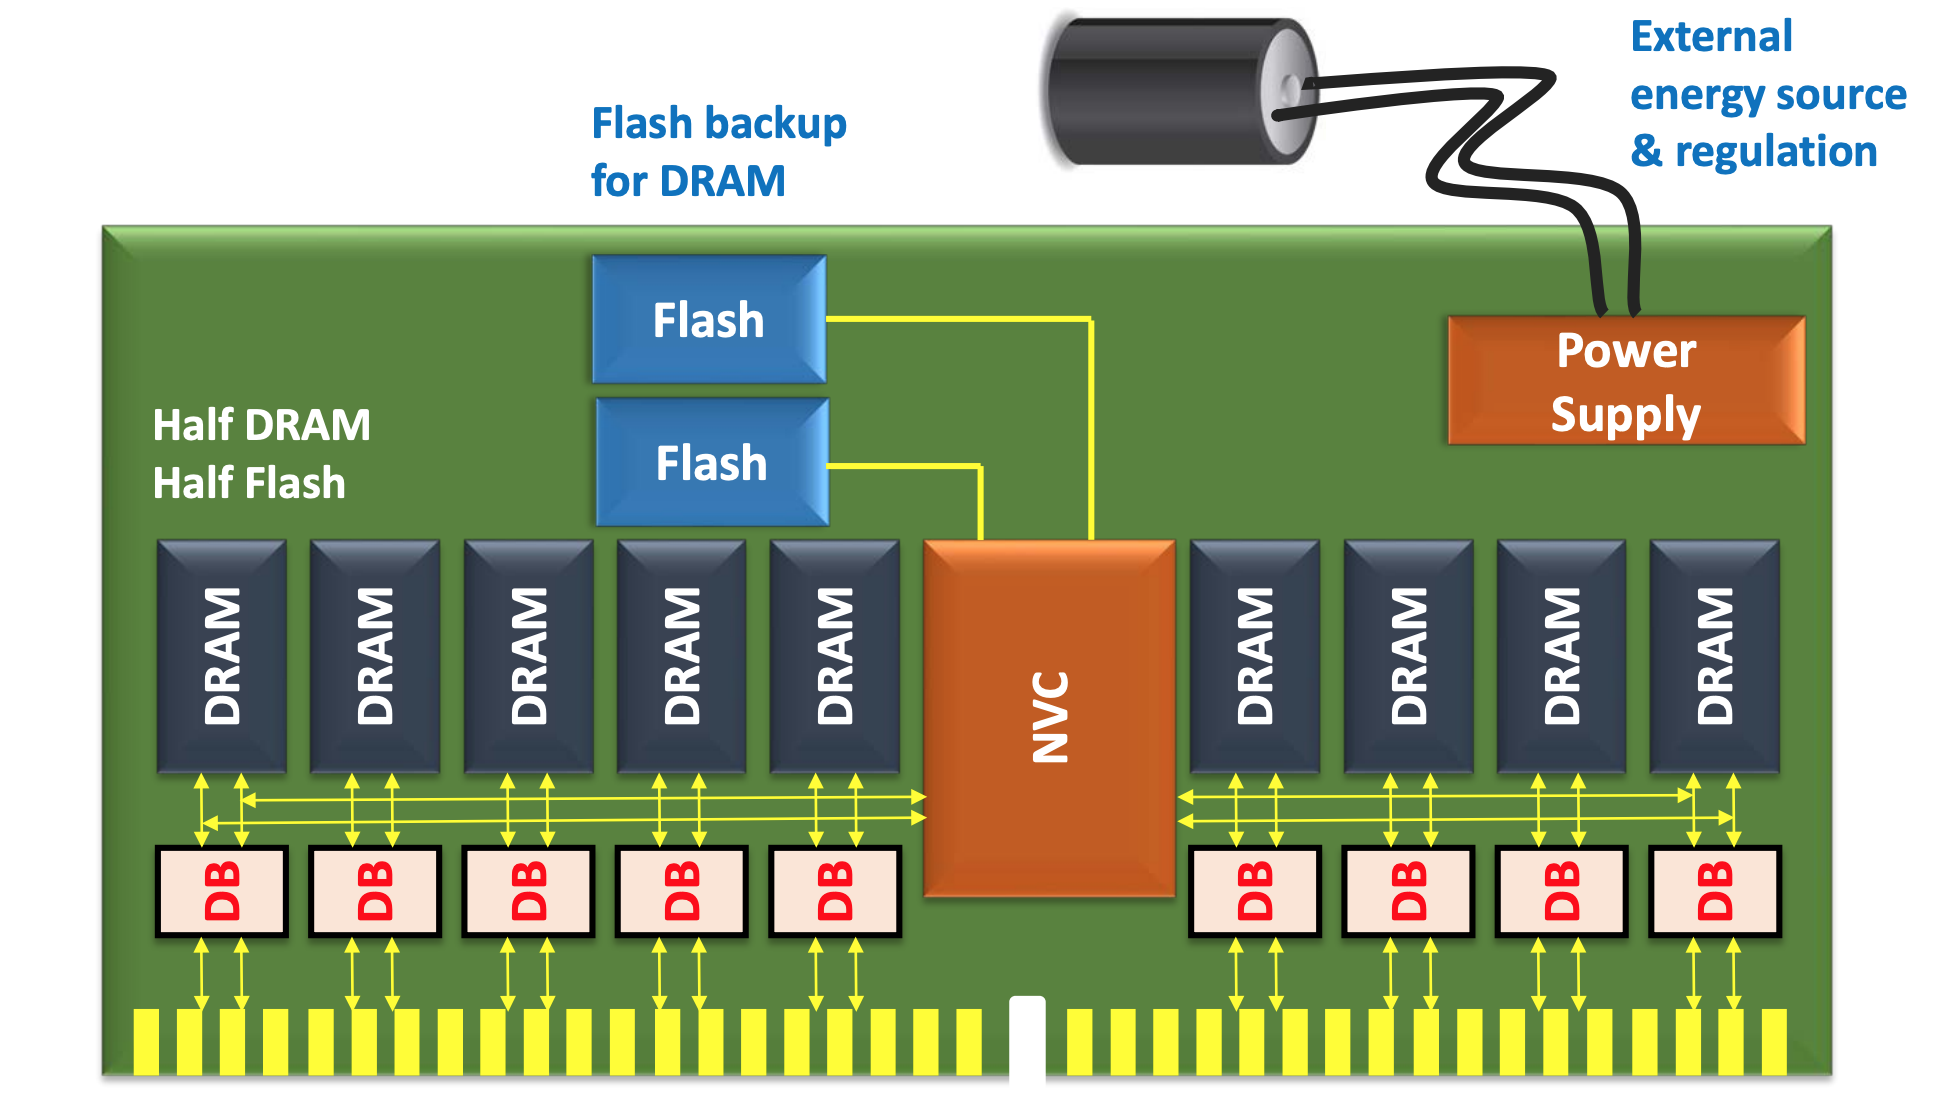
\includegraphics[width=\linewidth]{images/edl_nvdimm_n.png}
                    \caption{\label{fig:edl_nvdimm_n} NVDIMM-N}
                \end{subfigure}\hfill
                \begin{subfigure}[t]{0.50\textwidth}
                    \centering
                    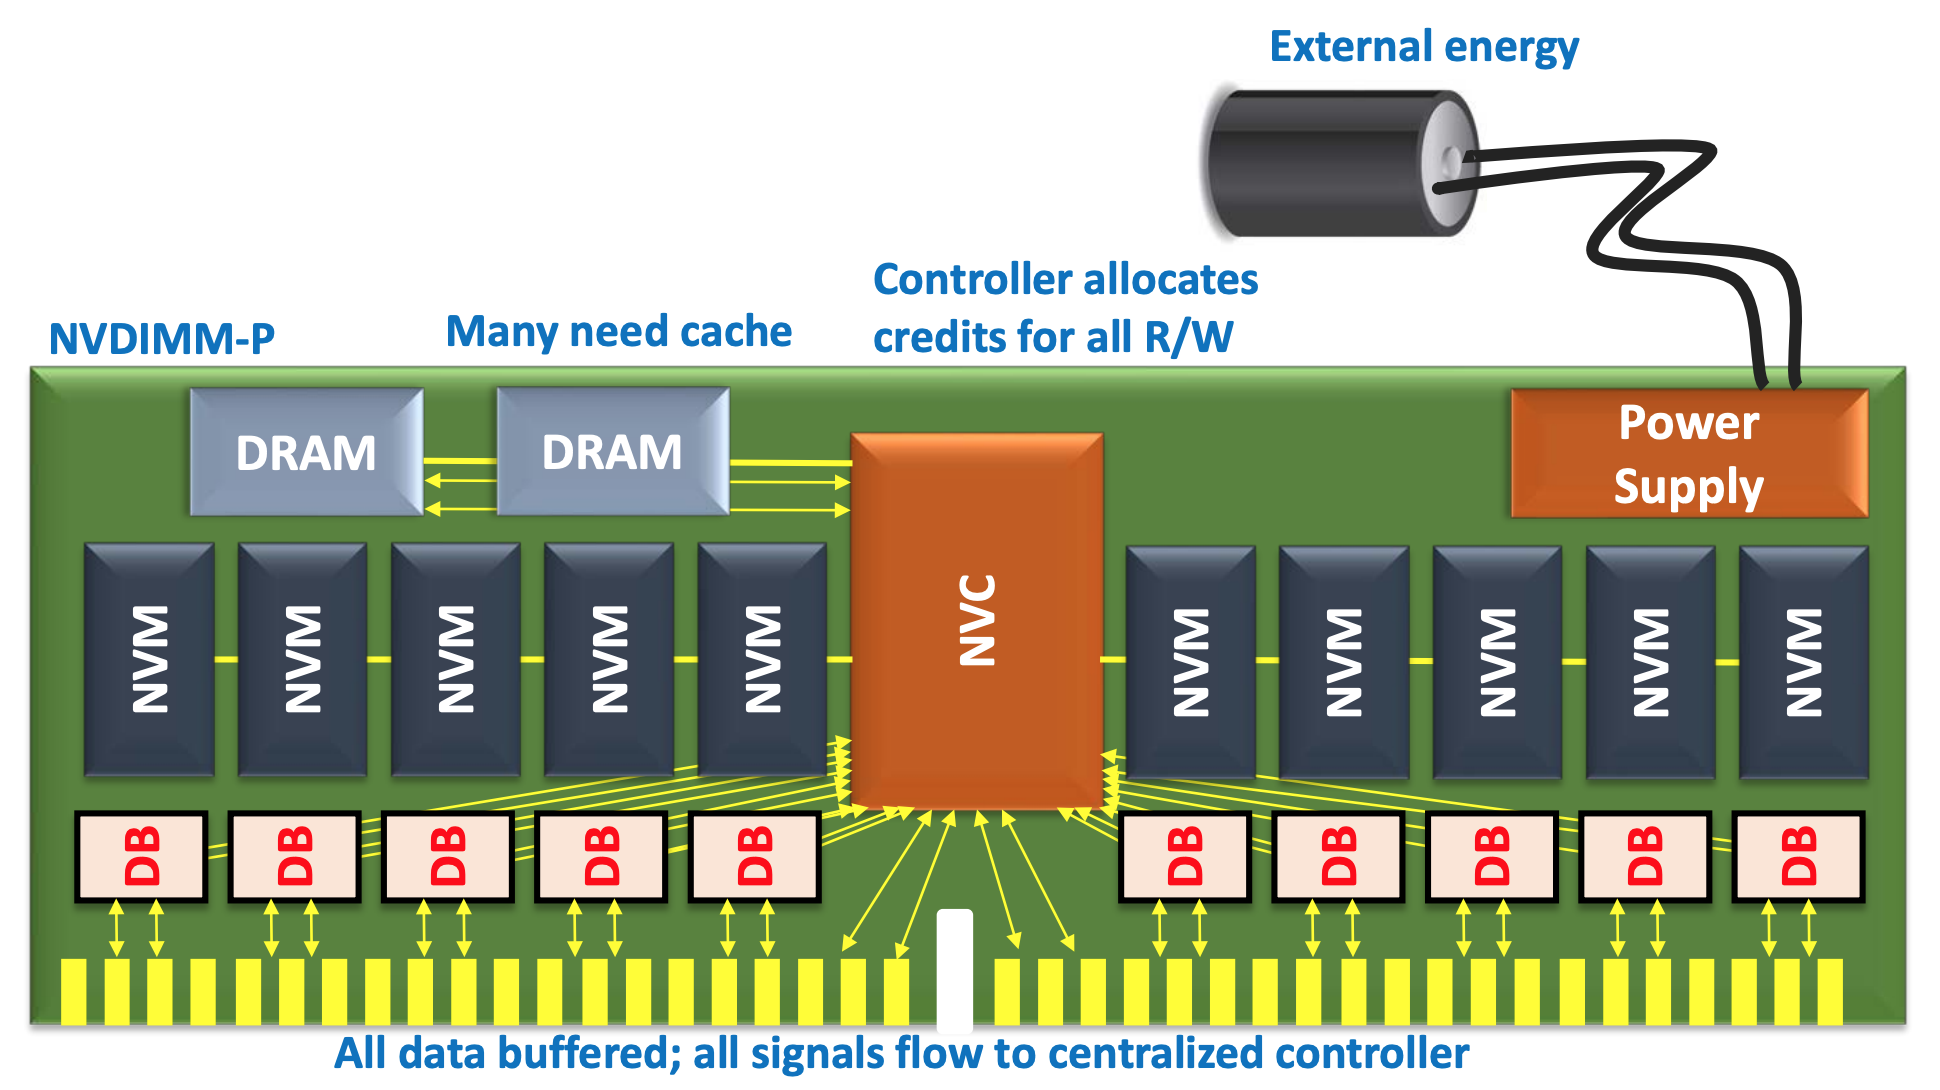
\includegraphics[width=\linewidth]{images/edl_nvdimm_p.png}
                    \caption{\label{fig:edl_nvdimm_p}NVDIMM-P}
                \end{subfigure}
                \caption{\label{fig:edl_nvdimm}Les deux standards NVDIMM développés par l'organisation JEDEC\protect\footnotemark.}
            \end{figure}
            \footnotetext{Source des illustrations: Bill Gervasi (Nantero) - \url{https://www.hotchips.org/hc30/2conf/2.04_Nantero_20180818_hotchips_gervasi_nram_presentation.pdf}}
        
        Le premier standard (Type 1) appelé NVDIMM-N (voir \autoref{fig:edl_nvdimm_n}) utilise de la mémoire DRAM associée à de la mémoire flash pour permettre la persistance des données ainsi qu'une source d'énergie indépendante permettant la sauvegarde des données en cas de coupure électrique. Lorsque le serveur est de nouveau alimenté, les données sont transférées de la mémoire flash à la DRAM pour permettre un redémarrage rapide. Pour l'utilisateur, la mémoire flash est invisible et ne peut pas être adressée. La capacité de ces mémoires aura tendance à être faible, car elles dépendent de la densité de la mémoire flash. Cependant, si la mémoire DRAM est bien utilisée, elle permet d'obtenir des performances et l'endurance proches d'une barrette de mémoire classique et bénéficie de la persistance grâce à la mémoire flash. 
            
        Le second standard (Type 3) appelé NVDIMM-F utilise seulement de la mémoire flash et est présenté au système d'exploitation comme un stockage. Cependant, contrairement à un disque classique, il bénéficie des performances du bus mémoire. Ce standard a depuis été abandonné. 
        
        Le troisième standard (Type 4) appelé NVDIMM-P (voir \autoref{fig:edl_nvdimm_p}) utilise de la mémoire DRAM associée à des technologies mémoires SCM (voir paragraphe suivant). Ces barrettes utilisent des banques de mémoires DRAM comme cache pour accélérer les communications avec les modules SCM. Le standard prévoit la possibilité d'adresser la mémoire en octets ou en blocs permettant des les utiliser comme mémoire, ou comme stockage. Les performances et la capacité de ce format de barrettes dépendent essentiellement des technologies SCM utilisées. C'est un avantage de ce type de NVDIMM, la technologie et le mode d'adressage utilisés pourront être adaptés en fonction des besoins des applications. Bien que la mémoire SCM soit non volatile, la barrette mémoire nécessite une alimentation pour sauver la contenue de la DRAM sur la SCM en cas de coupure électrique.

    \paragraph{Les Storage Class Memory (SCM)}\label{sec:SCM}
    %%%%%%%%%%%%%%%%%%%%%%%%%%%%%%%%%%%%%%%%%%%%%%%%%
    
        Les mémoires SCM regroupent toutes les nouvelles technologies développées répondant aux critères précédemment cités. La mémoire flash peut être considérée comme une SCM. Cependant, dans la littérature, le terme SCM est généralement utilisé pour désigner des technologies très innovantes aux caractéristiques supérieures à la flash. Cette technologie possède en effet quelques inconvénients qui ne permettront pas de l'utiliser comme une mémoire. Tout d'abord, ses performances asymétriques dont l'écriture est dix fois plus lente que la lecture. L'écriture et l'effacement ne peuvent se faire que par bloc. Enfin, l'endurance de la flash ne permet pas de supporter suffisamment d'écriture par cellule. En fonction des technologies utilisées (SLC, MLC, TLC) le nombre d'écritures par cellule est compris entre $10^3$ et $10^5$.  
        
        
        Dans la suite de cette section, nous présentons les technologies SCM ayant le plus de potentiel pour être industrialisé. En fonction des utilisations, certains types de mémoires seront préférés. Pour des applications de stockage, leur coût devra être proche de celui des disques, mais pourra avoir des latences plus élevées (inférieur à la microseconde) et des débits plus faibles (en centaines de mégaoctets/s). Cependant, leur endurance devra être la plus élevée possible ($10^{12}$ écritures). À terme, le prix des mémoires SCM devrait converger vers celui de la flash, permettant une utilisation massive dans les systèmes (voir \autoref{fig:edl_scm_evo}). Nous regroupons dans le \autoref{tab:SCM} les principales caractéristiques de ces technologies.
        
        
        \begin{figure}
        \center
        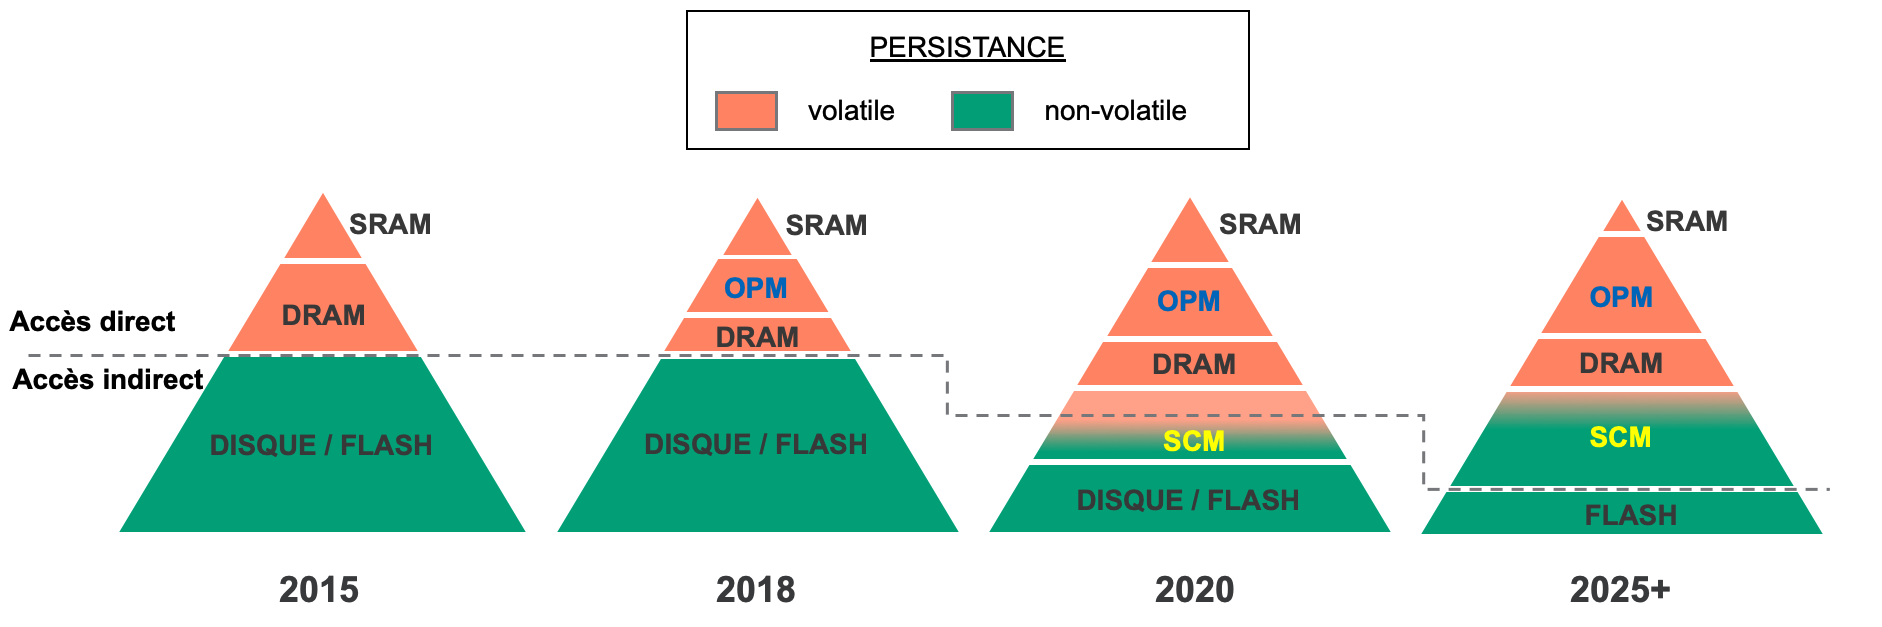
\includegraphics[width=17cm]{images/edl_scm_evo.png}
        \caption{\label{fig:edl_scm_evo} Évolution du système mémoire: les mémoires OPM (On Package Memory) telles que la HBM et les mémoires SCM (Storage Class Memory) vont permettre de compléter les trous de performance respectifs entre la SRAM et la DRAM ainsi qu'entre la DRAM et la flash.}
        \end{figure}
        
        
        \begin{table}[]
        \centering
        \resizebox{\textwidth}{!}{%
        \begin{tabular}{|l|c|c|c|c|c|c|c|c|}
        \hline
        \textbf{Technologies} & \textbf{DDR} & \textbf{NAND} & \textbf{3DXP PCM} & \textbf{MRAM} & \textbf{STT-RAM} & \textbf{FeRAM} & \textbf{RRAM} & \textbf{NRAM} \\ \hline
        \textbf{Persistance} & \cellcolor[HTML]{FD6864}Non & Oui & Oui & Oui & Oui & Oui & Oui & \cellcolor[HTML]{67FD9A}Oui \\ \hline
        \textbf{Endurance} & \cellcolor[HTML]{67FD9A}$10^{15}$ & \cellcolor[HTML]{FD6864}$10^{3}$-$10^{5}$ & \cellcolor[HTML]{FD6864}$10^{6}$ & $10^{12}$ & \cellcolor[HTML]{67FD9A}$10^{15}$ & \cellcolor[HTML]{67FD9A}$10^{14}$ & \cellcolor[HTML]{FD6864}$10^{6}$ & \cellcolor[HTML]{67FD9A}$10^{15}$ \\ \hline
        \textbf{Latence R/W} & \cellcolor[HTML]{67FD9A}10ns/10ns & 50us/25us & \cellcolor[HTML]{FD6864}100ns/1us & 50ns/1us & 50ns/100ns & 50ns/50ns & \cellcolor[HTML]{FD6864}200ns/1us & \cellcolor[HTML]{67FD9A}10ns/10ns \\ \hline
        \textbf{Énergie (pj)} & \cellcolor[HTML]{67FD9A}0.005 & \cellcolor[HTML]{FD6864}1360 & \cellcolor[HTML]{FFCC67}150 & 2 & 1 & 0.3 & \cellcolor[HTML]{FFCC67}64 & \cellcolor[HTML]{67FD9A}.005 \\ \hline
        \textbf{Densité} & moyenne & \cellcolor[HTML]{67FD9A}haute & moyenne & faible & faible & faible & moyenne & moyenne \\ \hline
        \textbf{Rétention} & \cellcolor[HTML]{FD6864}4us & 1 an & 10 ans & \cellcolor[HTML]{FFCC67}jours & \cellcolor[HTML]{FFCC67}jours & 10 ans & 10 ans & \cellcolor[HTML]{67FD9A}10 ans \\ \hline
        \textbf{Adressabilité} & byte & \cellcolor[HTML]{FD6864}Page & byte & byte & byte & byte & byte & byte \\ \hline
        \textbf{Scalabilité} & 16nm & \cellcolor[HTML]{67FD9A}QLC, 96L+ & \textless{}20nm & 28nm & 28nm & \cellcolor[HTML]{FD6864}40nm & \textless{}20nm & \cellcolor[HTML]{67FD9A}\textless{}10nm \\ \hline
        \textbf{Price /GB} & \cellcolor[HTML]{FFCC67}7\$ & \cellcolor[HTML]{67FD9A}\textless{}1\$ & 3.5\$ & \cellcolor[HTML]{FD6864}2K\$ & \cellcolor[HTML]{FD6864}4K\$ & \cellcolor[HTML]{FD6864}32K\$ & 3.5\$ & \cellcolor[HTML]{FFCC67}6\$ \\ \hline
        \textbf{Status} & Prod. & Prod. & Prod. & Prod. & Prod. & \cellcolor[HTML]{FFCC67}Prod. / fin & \cellcolor[HTML]{FD6864}échantillon & \cellcolor[HTML]{FD6864}échantillon \\ \hline
        \end{tabular}%
        }
        \caption{État de l'art des différentes technologies SCM comparées à la DRAM et à la mémoire flash.}
        \label{tab:SCM}
        \end{table}
        
        Le développement de ces technologies n'est pas récent. On retrouve par exemple un article sur le développement de \textbf{mémoire PCM} (mémoire à changement de phase) daté de 1969 \cite{Sie1969}. C'est notamment la technologie utilisée pour les mémoires XPoint d'Intel \cite{Handy2015}. Elle utilise certaines propriétés des matériaux chalcogénures tels que la photosensibilité ou la résistivité électrique. Ces matériaux peuvent basculer entre deux phases sous l’effet de la chaleur influant sur leur conductivité permettant d'encoder l'information. Le matériau peut être chauffé de deux façons: à l'aide d'un laser (utilisé pour les disques optiques réinscriptibles (CD-RW)) ou en utilisant l'effet joule. La lecture se fait ensuite en mesurant sa résistance à l'aide d'un courant suffisamment faible pour ne pas modifier son état. Ces mémoires, insensibles aux radiations sont particulièrement intéressantes pour les situations particulières telles que l'aérospatiale. \textbf{La MRAM} (\textit{RAM magnétique}) utilise le spin des électrons.  Suivant leur orientation par rapport à un aimant, la résistance change et permet de stocker l'information. En 2003, IBM a produit le premier démonstrateur en produisant la première mémoire MRAM de 128kb  \cite{Bette2003}. Depuis, d'autres constructeurs ont produit de tels mémoires comme Freescale (un million de puces vendues), ainsi que Samsung et Hynix. Le futur de cette technologie est d'évoluer en STT-RAM \cite{Alvarez-Herault2010} (\textit{spin transfer torque} MRAM) permettant d'atteindre des densités d'intégrations plus élevées, une latence réduite proche de celle de la DRAM. Grâce à une consommation électrique faible, cette mémoire pourrait être adaptée pour les objets connectés (IOT). \textbf{La FeRAM} ou Mémoire Ferroélectrique à accès aléatoires possède la même structure que la DRAM avec un matériau ferroélectrique à la place du diélectrique stockant l’information. Cette technologie permettrait de profiter de la simplicité de la DRAM avec une intégration plus élevée (moins que la mémoire flash \cite{Alvarez-Herault2010}). Beaucoup de problèmes sont rencontrés dans leur fabrication, notamment la pollution du silicone par le PZT. \textbf{La NRAM} (Nano RAM) repose sur l'utilisation de nanotubes de carbone. Un réseau de tubes croisés est activé électrostatiquement à l'aide d'une différence de potentiel pour faire fléchir les tubes et les mettre en contacte ou non \cite{Ricart2008}. Ses performances proches de celles de la DRAM en font un excellent remplacement.  La production de cette technologie est relativement simple et elle peut être empilée pour augmenter sa densité \cite{Gervasi2019}. \textbf{La ReRAM} (RAM résistive) se base sur le déplacement de trous dans des cristaux dopés. La production de cette mémoire est relativement simple et permettrait d'obtenir des prix compétitifs. Le désavantage de cette mémoire est la faible endurance aux écritures proche de celui de la flash. Le développement de cette technologie n'est pas encore terminé, et ne serait pas annoncé avant 2025.
        
        
        



\newpage


\subsection{Nouvelles technologies d'interconnexion.}
%%%%%%%%%%%%%%%%%%%%%%%%%%%%%%%%%%%%%%%%%%%%%%%%%%    

    Dans la section précédente, nous avons discuté du besoin de développer de nouvelles technologies mémoires. Cependant, pour pouvoir profiter de débits plus élevés que ceux atteints actuellement, il est indispensable de développer de nouvelles technologies pour améliorer la performance du bus mémoire et du système d'interconnexion. Dans cette section, nous étudions les débits du bus mémoire et la consommation énergétique du système d'interconnexion des plateformes actuelles. Nous présentons ensuite de nouvelles technologies pouvant être utilisées. 

    \subsubsection{Débit mémoire des processeurs} 
        
        Nous proposons d'étudier l'utilisation d'un processeur Intel Skylake pour l'exécution d'applications HPC typiques. Un tel processeur possédant 28 coeurs cadencés à 2.3 GHz, réalise en performance crête 2 TFLOPS (voir détail du calcul dans la \autoref{sec:methodo_step1}). En supposant l'utilisation d'un bus mémoire délivrant 100 Gb/s, nous calculons le débit de donnée transférable pour chaque opération exécutée:
        \begin{equation}
            \frac{100 \times 10^9 \; byte/s}{2 \times 10^{12} \; FLOP/s} = 0.05 \; byte/FLOP
        \end{equation}
        Ce résultat signifie que pendant l'exécution d'une opération, le système mémoire est capable de transférer 0.05 byte de la mémoire au processeur. Les applications de simulation numérique, telle que celles utilisées dans le domaine de la recherche pétrolière basée sur des algorithmes de Stencil, ont besoin de transférer depuis la mémoire 2 bytes par FLOP (4 pour l'application HPCG\footnote{Report on the HPC application bottlenecks - \url{http://exanode.eu/wp-content/uploads/2017/04/D2.5.pdf}}), l'idéal se trouvant autour des 8 bytes par opération \cite{Bergman2015}. Cette valeur est estimée pour un algorithme utilisant parfaitement la localité des mémoires caches et utilisant des opérations en double précision. On remarque donc que le système mémoire est très loin d'être capable de délivrer suffisamment de données pour permettre au processeur d'atteindre sa puissance crête (facteur 40). 
        
    %%%%%%%%%%%%%%%%%%%%%%%%%%%%%%%%%%%%%%%%%%%%%%%%%%%%%%%%%%%%%%%
    
    \subsubsection{Consommation du système d'interconnexion} 
        
        Les applications de calculs parallèles doivent échanger certains résultats entre serveurs. Il est courant d'utiliser des valeurs entre $0.1$ et $0.2 \; byte/FLOP$ \cite{Bergman2015} pour des applications de simulation numérique. Pour pouvoir fournir suffisamment de données aux serveurs, la plateforme exascale devrait utiliser un système d'interconnexion avec un débit équivalent à:
        \begin{equation}
            0.2 \; byte/FLOP \times 10^{18} \; FLOP/s = 200 \times 10^{15} \; byte/s
        \end{equation}
        Les plateformes du Top500 allouent autour de 15\% de leur budget énergétique totale \cite{bergman2008exascale}, pour l'alimentation du système d'interconnexion. Pour une plateforme Exascale consommant 20 MW cela correspond à une enveloppe énergétique de 3 MW. Nous pouvons ainsi calculer le budget d'énergie utilisable pour le transfert de chaque donnée:
        \begin{equation}
            \frac{3 * 10^6 \; joule/s}{200 * 10^{15} \; byte/s} = 15 \; pj/byte = 1.87 \; pj/bit
        \end{equation}
        Cette énergie représente l'enveloppe énergétique totale utilisable pour transférer un bit d'informations entre deux noeuds du système. Ce transfert comprend le passage dans les différents commutateurs. Nous avons étudié dans la \autoref{sec:edl_chal_energie} que le budget actuellement nécessaire pour un tel transfère dépassait 1000 pj/bit.
    
    %%%%%%%%%%%%%%%%%%%%%%%%%%%%%%%%%%%%%%%%%%%%%%%%%%%%%%%%%%%%%%%
    
    \subsubsection{Objectifs des nouvelles technologies d'interconnexion} 
        
        Nous constatons donc le besoin de nouvelles technologies d'interconnexion. Les évolutions de plusieurs facteurs nécessaires ne pourront pas provenir d'une simple évolution des technologies actuellement utilisées:
        \begin{itemize}
            \item \textbf{La consommation électrique} doit être réduite de plusieurs facteurs, non seulement pour le système d'interconnexion, mais aussi pour les accès mémoires. La programmation d'algorithmes efficaces (localité) est alors primordiale. 
            \item \textbf{Les débits mémoires} offerts doivent être améliorés de plusieurs facteurs pour pouvoir alimenter les processeurs et les accélérateurs. 
            \item \textbf{La latence} du système d'interconnexion devra être la plus faible possible pour permettre à certaines applications de générer des accès mémoire imprédictibles (parcours de graphes). Les jeux de données ne pouvant pas être stockés sur une seule machine, le système d'interconnexion doit posséder une latence très faible pour pouvoir accéder rapidement à une donnée distante.
        \end{itemize}
    
    %%%%%%%%%%%%%%%%%%%%%%%%%%%%%%%%%%%%%%%%%%%%%%%%%%%%%%%%%%%%%%%%%%%%%%%
    
    \subsubsection{La photonique}
    
        Afin de répondre aux challenges exposés précédemment, l'industrie du HPC s'est lancée depuis plusieurs dizaines d'années dans la recherche et le développement de technologies photoniques. La photonique est un domaine de la physique qui a pour objectif de manipuler la lumière (photon): l'émission, la transmission, la captation et le traitement. Les premiers émetteurs ont été développés dans les années 1960. Aujourd'hui, la photonique à de nombreuses applications: lecteur de code-barre et DVD, illumination LED, vision nocturne\ldots Dans le domaine des télécommunications, l'application la plus connue est la fibre optique. L'utilisation de technologies photoniques dans les supercalculateurs à deux avantages principaux répondant aux besoins évoqués ci-dessus.
       
        \begin{itemize}
            \item \textbf{L'indépendance à la distance} est le premier avantage de la photonique. Que ce soit en termes de latence ou de consommation électrique, la photonique permet de \textit{réduire les distances} d'un supercalculateur. En effet, la génération d'un signal optique ou électronique nécessite une quantité d'énergie similaire. Cependant, pour les technologies photoniques, celle-ci évolue faiblement avec la distance de communication (\autoref{fig:edl_photo_pj}). Lorsque les accès sont proches (sur la puce), il n'y a pas d'avantages en terme énergétique à utiliser la technologie photonique. Cependant, une fois les photons générés, le coût énergétique ne varie que faiblement avec la distance d'accès, et cela jusqu'à plusieurs centaines de mètres. Ainsi, le coût énergétique d'un accès mémoire est proche de celui d'un accès à une mémoire distante située sur un autre serveur. Pour ces accès, la photonique permet de réduire la consommation électrique de plusieurs ordres. 
    
            \item \textbf{Les débits mémoire}s atteignables par l'utilisation de la photonique sont le deuxième avantage. À la différence des signaux électriques qui interfèrent lorsqu’ils sont utilisés sur une même broche, il est possible d’accumuler plusieurs signaux de différentes longueurs d’onde sur le même guide d’onde (\textit{wave guide}). Il est ainsi possible d'atteindre une haute densité de communication (voir \autoref{fig:edl_photo_bw}). Ces technologies peuvent atteindre des débits de 800 Gb/s avec une consommation de 2.2 pj/bit. Les prochaines générations permettront d'atteindre des débits de 1 Tb/s  avec une consommation de 1 pj/bit \cite{Bergman2018}. Cette faible densité va permettre d'utiliser la photonique à l'intérieur des puces permettant d'atteindre des débits élevés pour par exemple connecter une mémoire HBM au processeur.
        \end{itemize}
        
        
        \begin{figure}[t!]
            \centering
            \begin{subfigure}[t]{0.48\textwidth}
                \centering
                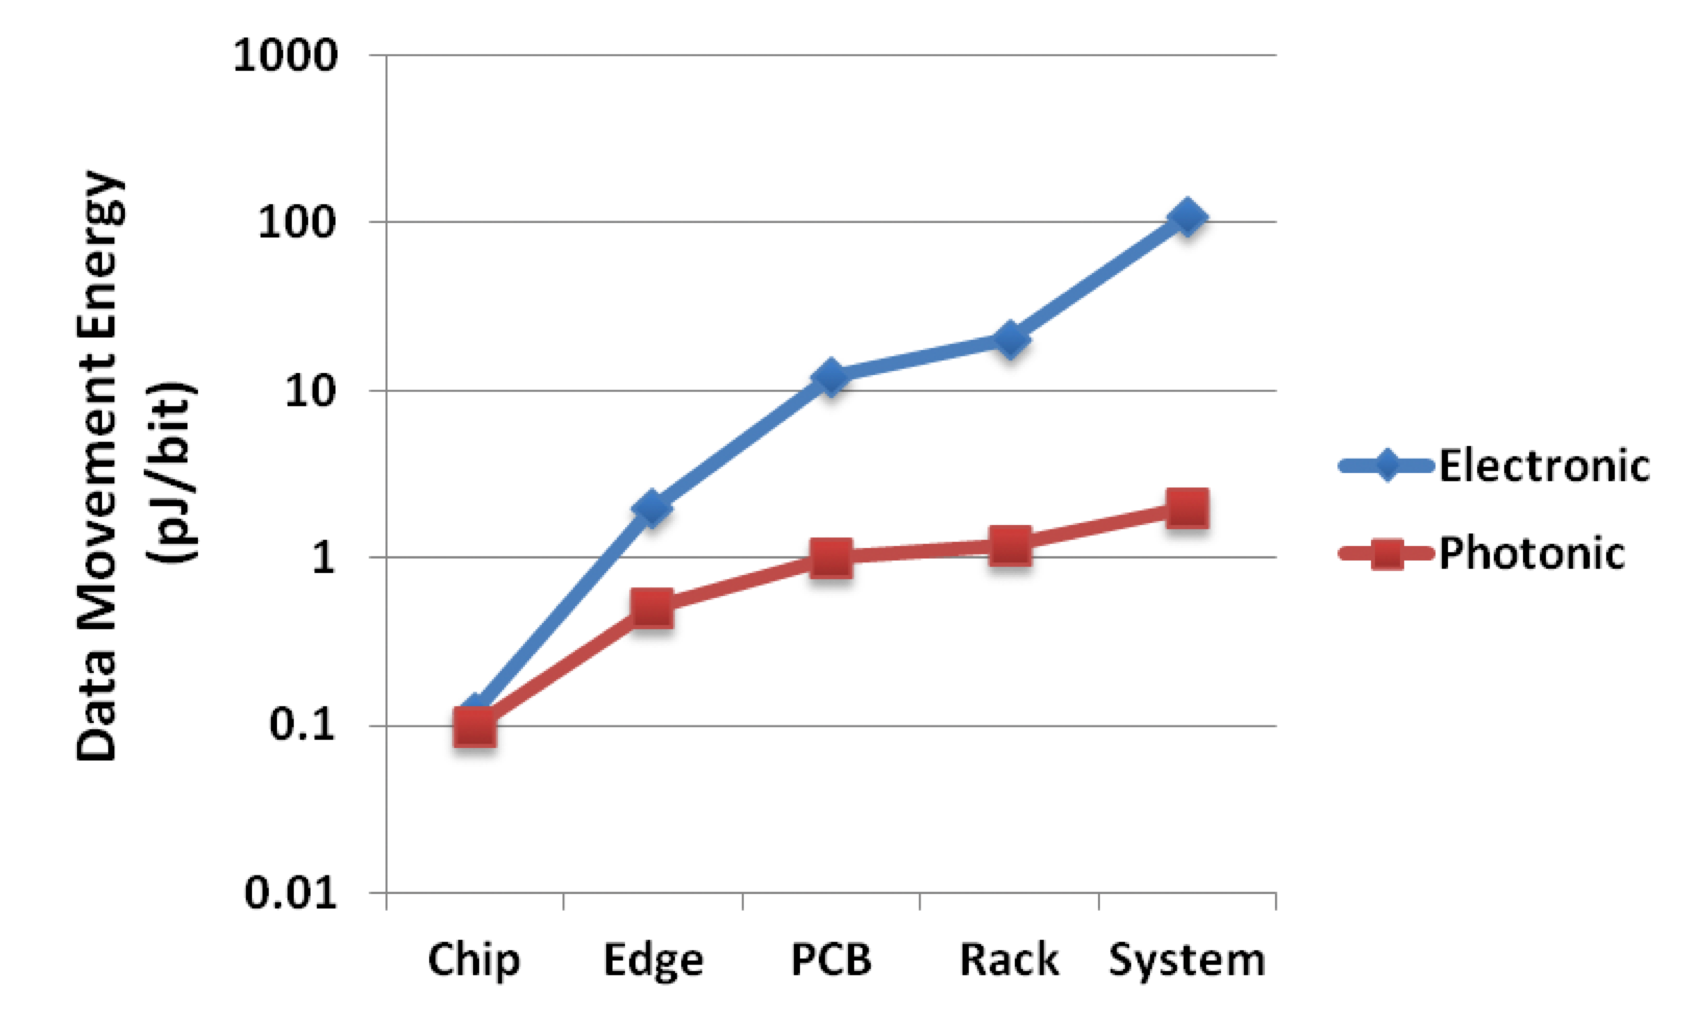
\includegraphics[width=\linewidth]{images/edl_photo_pj.png}
                \caption{\label{fig:edl_photo_pj} Distance d'accès et débit mémoire.}
            \end{subfigure}\hfill
            \begin{subfigure}[t]{0.48\textwidth}
                \centering
                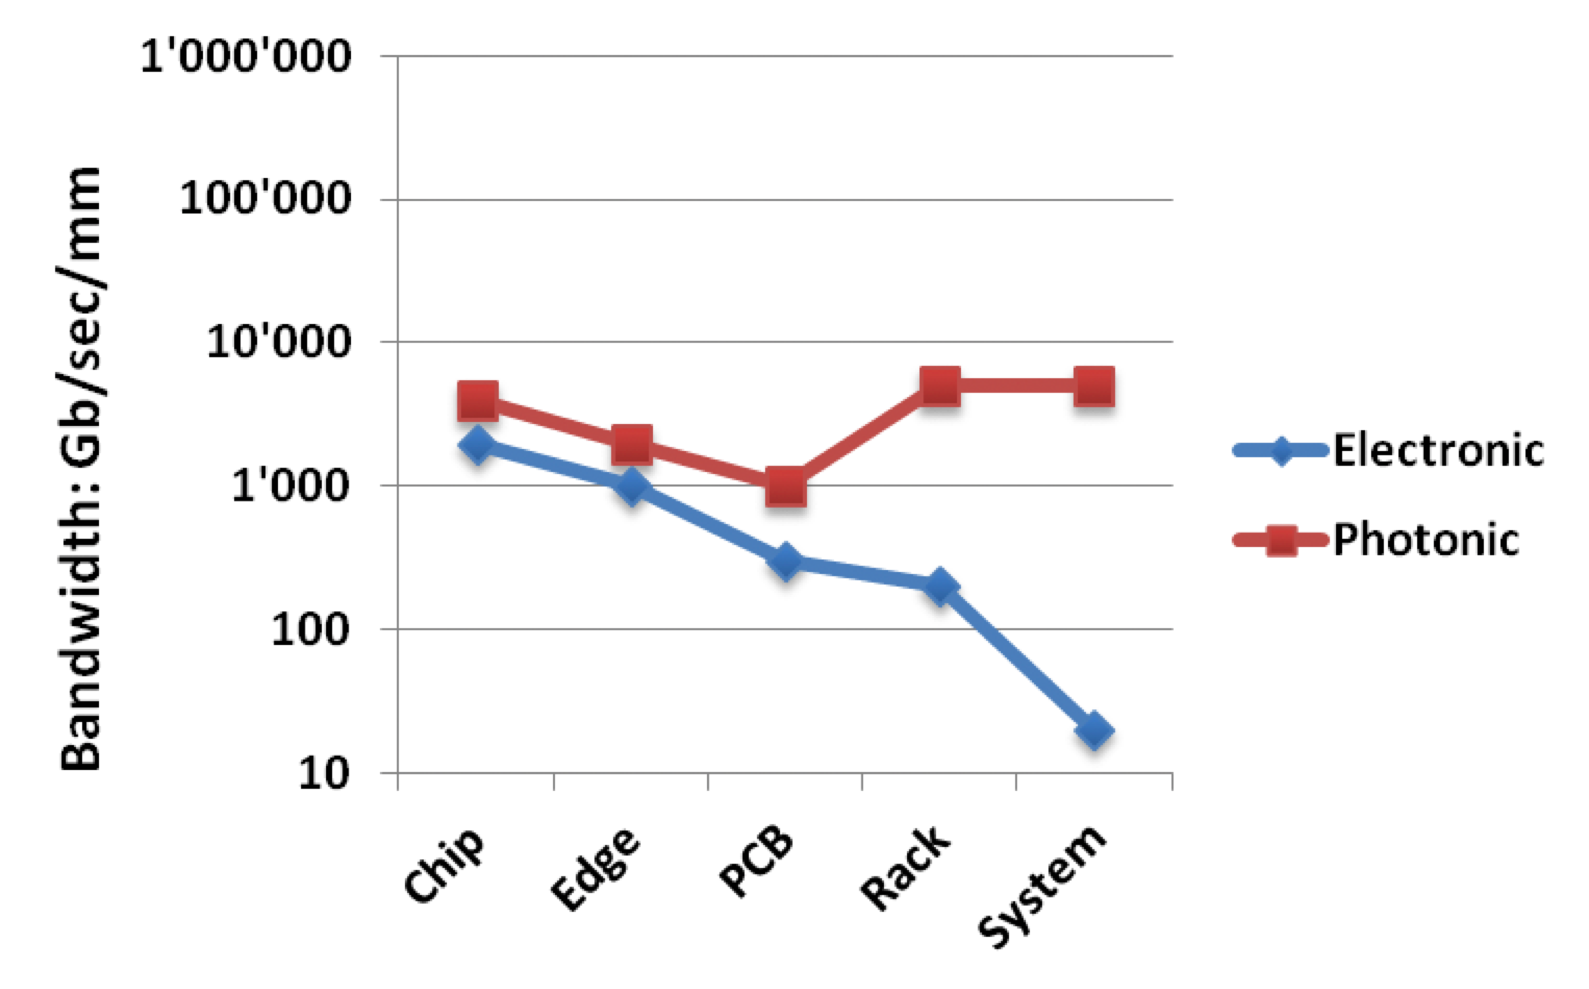
\includegraphics[width=\linewidth]{images/edl_photo_bw.png}
                \caption{\label{fig:edl_photo_bw} Distance d'accès et consommation électrique.}
            \end{subfigure}
            \caption{\label{fig:edl_photo} La transmission par photonique a deux avantages principaux comparés à la transmission électronique\cite{Lucas2014}}
        \end{figure}
    
    
        % Nouveaux usages
        L'utilisation des technologies photoniques dans les supercalculateurs va permettre de \textit{réduire} les distances en améliorant les latences de communication ainsi qu'en réduisant les coûts énergétiques. Il sera donc presque équivalent de communiquer avec sa propre mémoire, qu'avec celle d'un serveur situé à l'autre bout du centre de données. Ainsi, les supercalculateurs utilisés par plusieurs utilisateurs subiront moins les effets de fragmentation, car il n'y aura plus d'inconvénient à utiliser des machines distantes. Cependant, la topologie des calculateurs va devoir être repensée pour exploiter cette caractéristique (voir \autoref{sec:gen_z}).
        
        
        %ANNEAUX 
        De nombreuses technologies sont développées pour rendre possible l'utilisation de la photonique dans les centres de données. Par exemple, en utilisant des anneaux résonnants directement sur les puces silicium (voir \autoref{fig:edl_photo_ring_prez}). Ces anneaux sont des guides d’onde bouclés, permettant, pour une longueur d'onde donnée, de générer une résonance et propager l'onde dans celui-ci. Pour pouvoir contrôler les signaux, différents types d'anneaux ont été développés (voir \autoref{fig:edl_photo_ring}). Chaque anneau à une fonctionnalité permettant de réaliser différentes opérations: laisser passer ou non un signal, le commuter ou encore détecter la présence d'une certaine longueur d'onde. D'autres types d'anneaux sont utilisés pour générer les signaux et permettent d'encoder les informations à transmettre. En combinant ces anneaux, il est possible de développer des composants complexes comme des commutateurs.
        
        \begin{figure}[t!]
            \centering
            \begin{subfigure}[t]{0.48\textwidth}
                \centering
                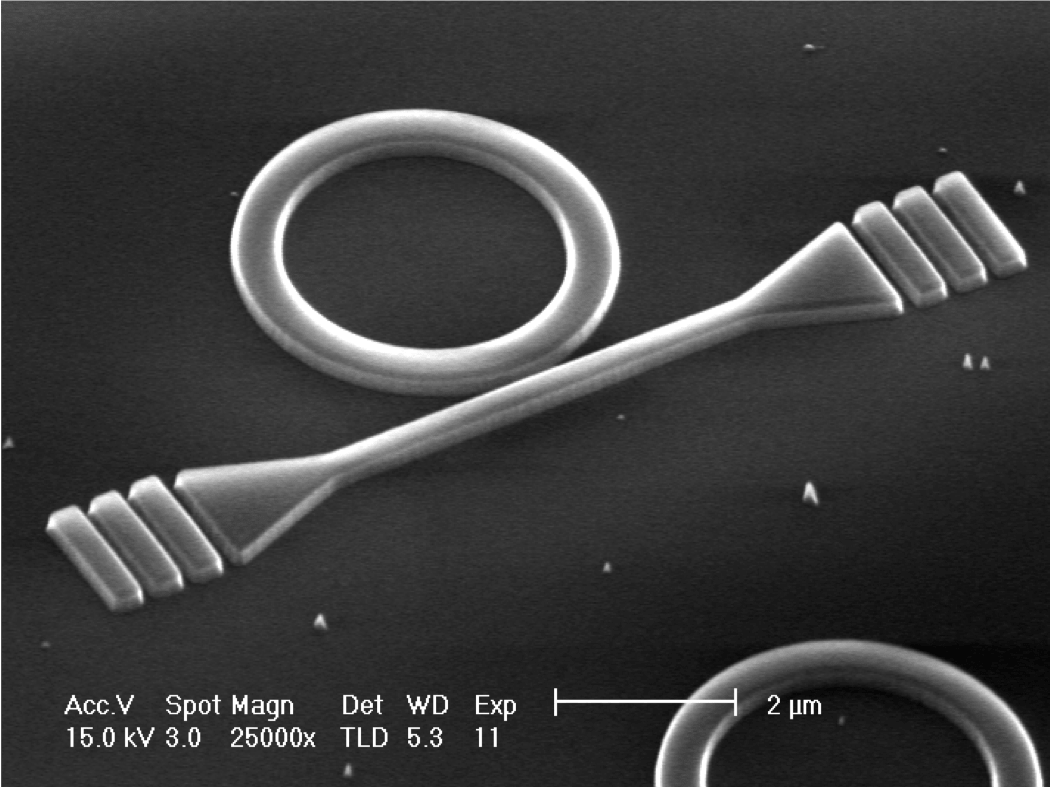
\includegraphics[width=\linewidth]{images/edl_photo_ring1.png}
                \caption{\label{fig:edl_photo_ring1} Anneau résonnant vu au microscope.}
            \end{subfigure}\hfill
            \begin{subfigure}[t]{0.40\textwidth}
                \centering
                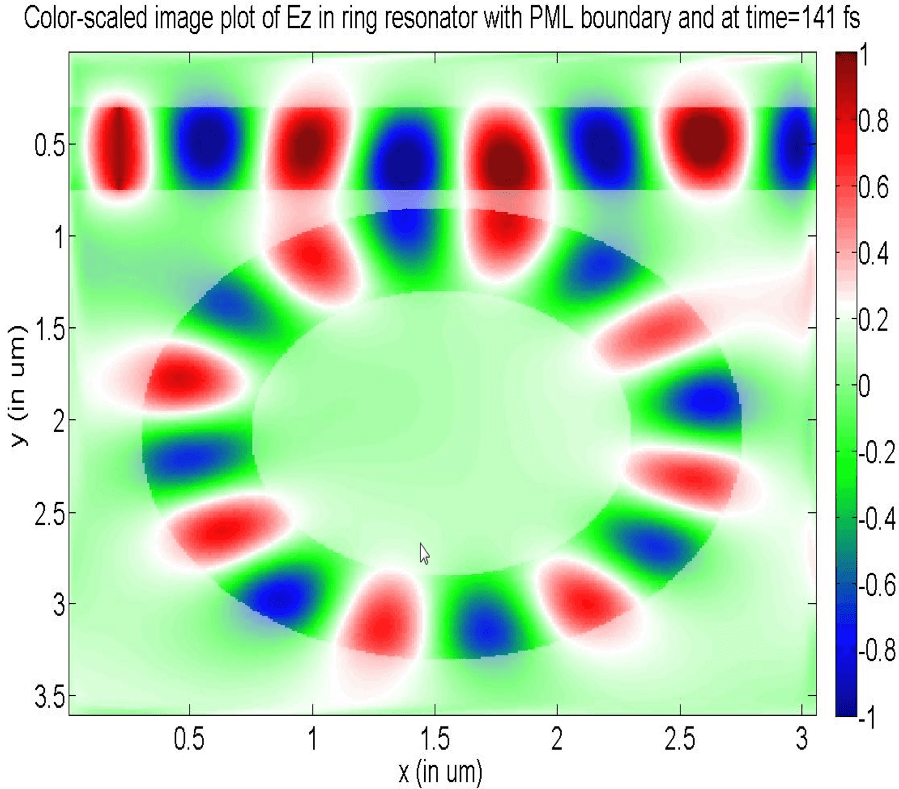
\includegraphics[width=\linewidth]{images/edl_photo_ring2.png}
                \caption{\label{fig:edl_photo_ring1} Fonctionnement d'un anneau résonnant}
            \end{subfigure}
            \caption{\label{fig:edl_photo_ring_prez} Illustration d'un anneau résonnant}
        \end{figure}
        
        \begin{figure}
            \center
            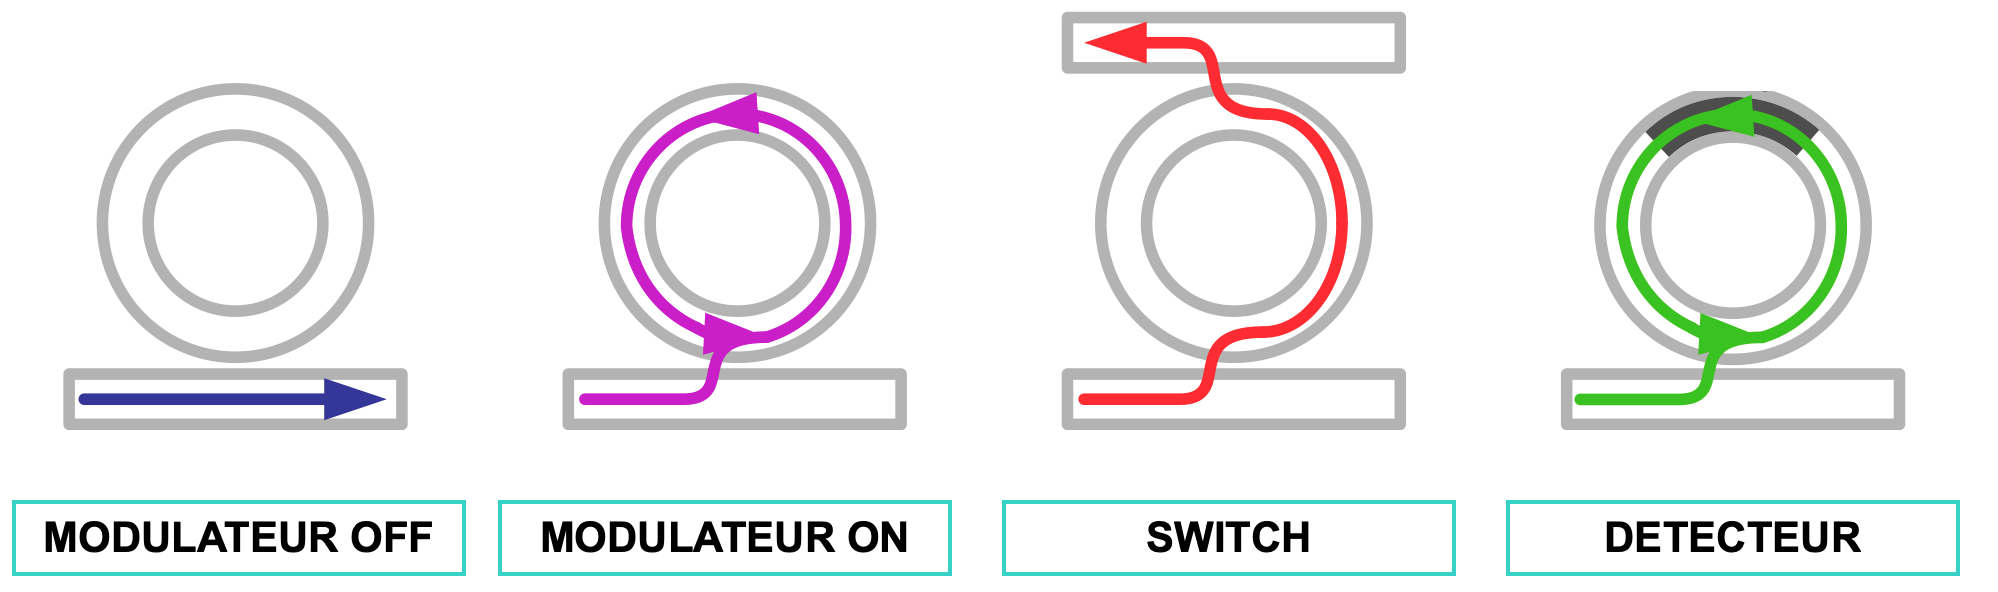
\includegraphics[width=14cm]{images/edl_photo_ring.png}
            \caption{\label{fig:edl_photo_ring} Différents types de résonateur en anneau.}
        \end{figure}


\subsection{Nouvelles architectures}\label{sec:new_soc}
%%%%%%%%%%%%%%%%%%%%%%%%%%%%%%%%%%%%%%%%%%%%%%%%%%%
    
    Dans cette section nous présentons les nouvelles architectures et les méthodes employées pour améliorer les performances des processeurs et des accélérateurs utilisés dans les supercalculateurs. Pour cela nous présentons la méthode de \textit{co-desing} et présentons quelques architectures novatrices. Enfin, nous  discutons de la nécessité d'avoir des architectures hétérogènes pour atteindre l'efficience énergétique espérée.
    
    \subsubsection{Codesign.}\label{sec:codesign}
        
        En informatique, le co-design (ou co-conception) est un processus de conception de système informatique impliquant différents acteurs: fabricant, programmeurs, utilisateurs finaux. Ce processus a pour objectif d'influencer la conception des architectures et le développement de technologies en tenant compte des besoins logiciels et algorithmiques. Il regroupe autour de partenariat longue durée l'expertise des fournisseurs, des architectes, des scientifiques et des programmeurs dans le but de développer les meilleures technologies possible en fonction des besoins exprimés (coût, performance, efficacité énergétique). Le co-design est une piste majeure pour le développement de processeurs et d'accélérateurs ultras optimisés utilisés dans l'élaboration de plateformes \gls{exascale}. La motivation principale étant réfléchir à la façon de développer une plateforme exascale répondant aux besoins des applications plutôt que de se demander quelles applications sont adaptées à cette plateforme une fois celle-ci développée \cite{PARKERe2013}.
        
        \begin{figure}
        \center
        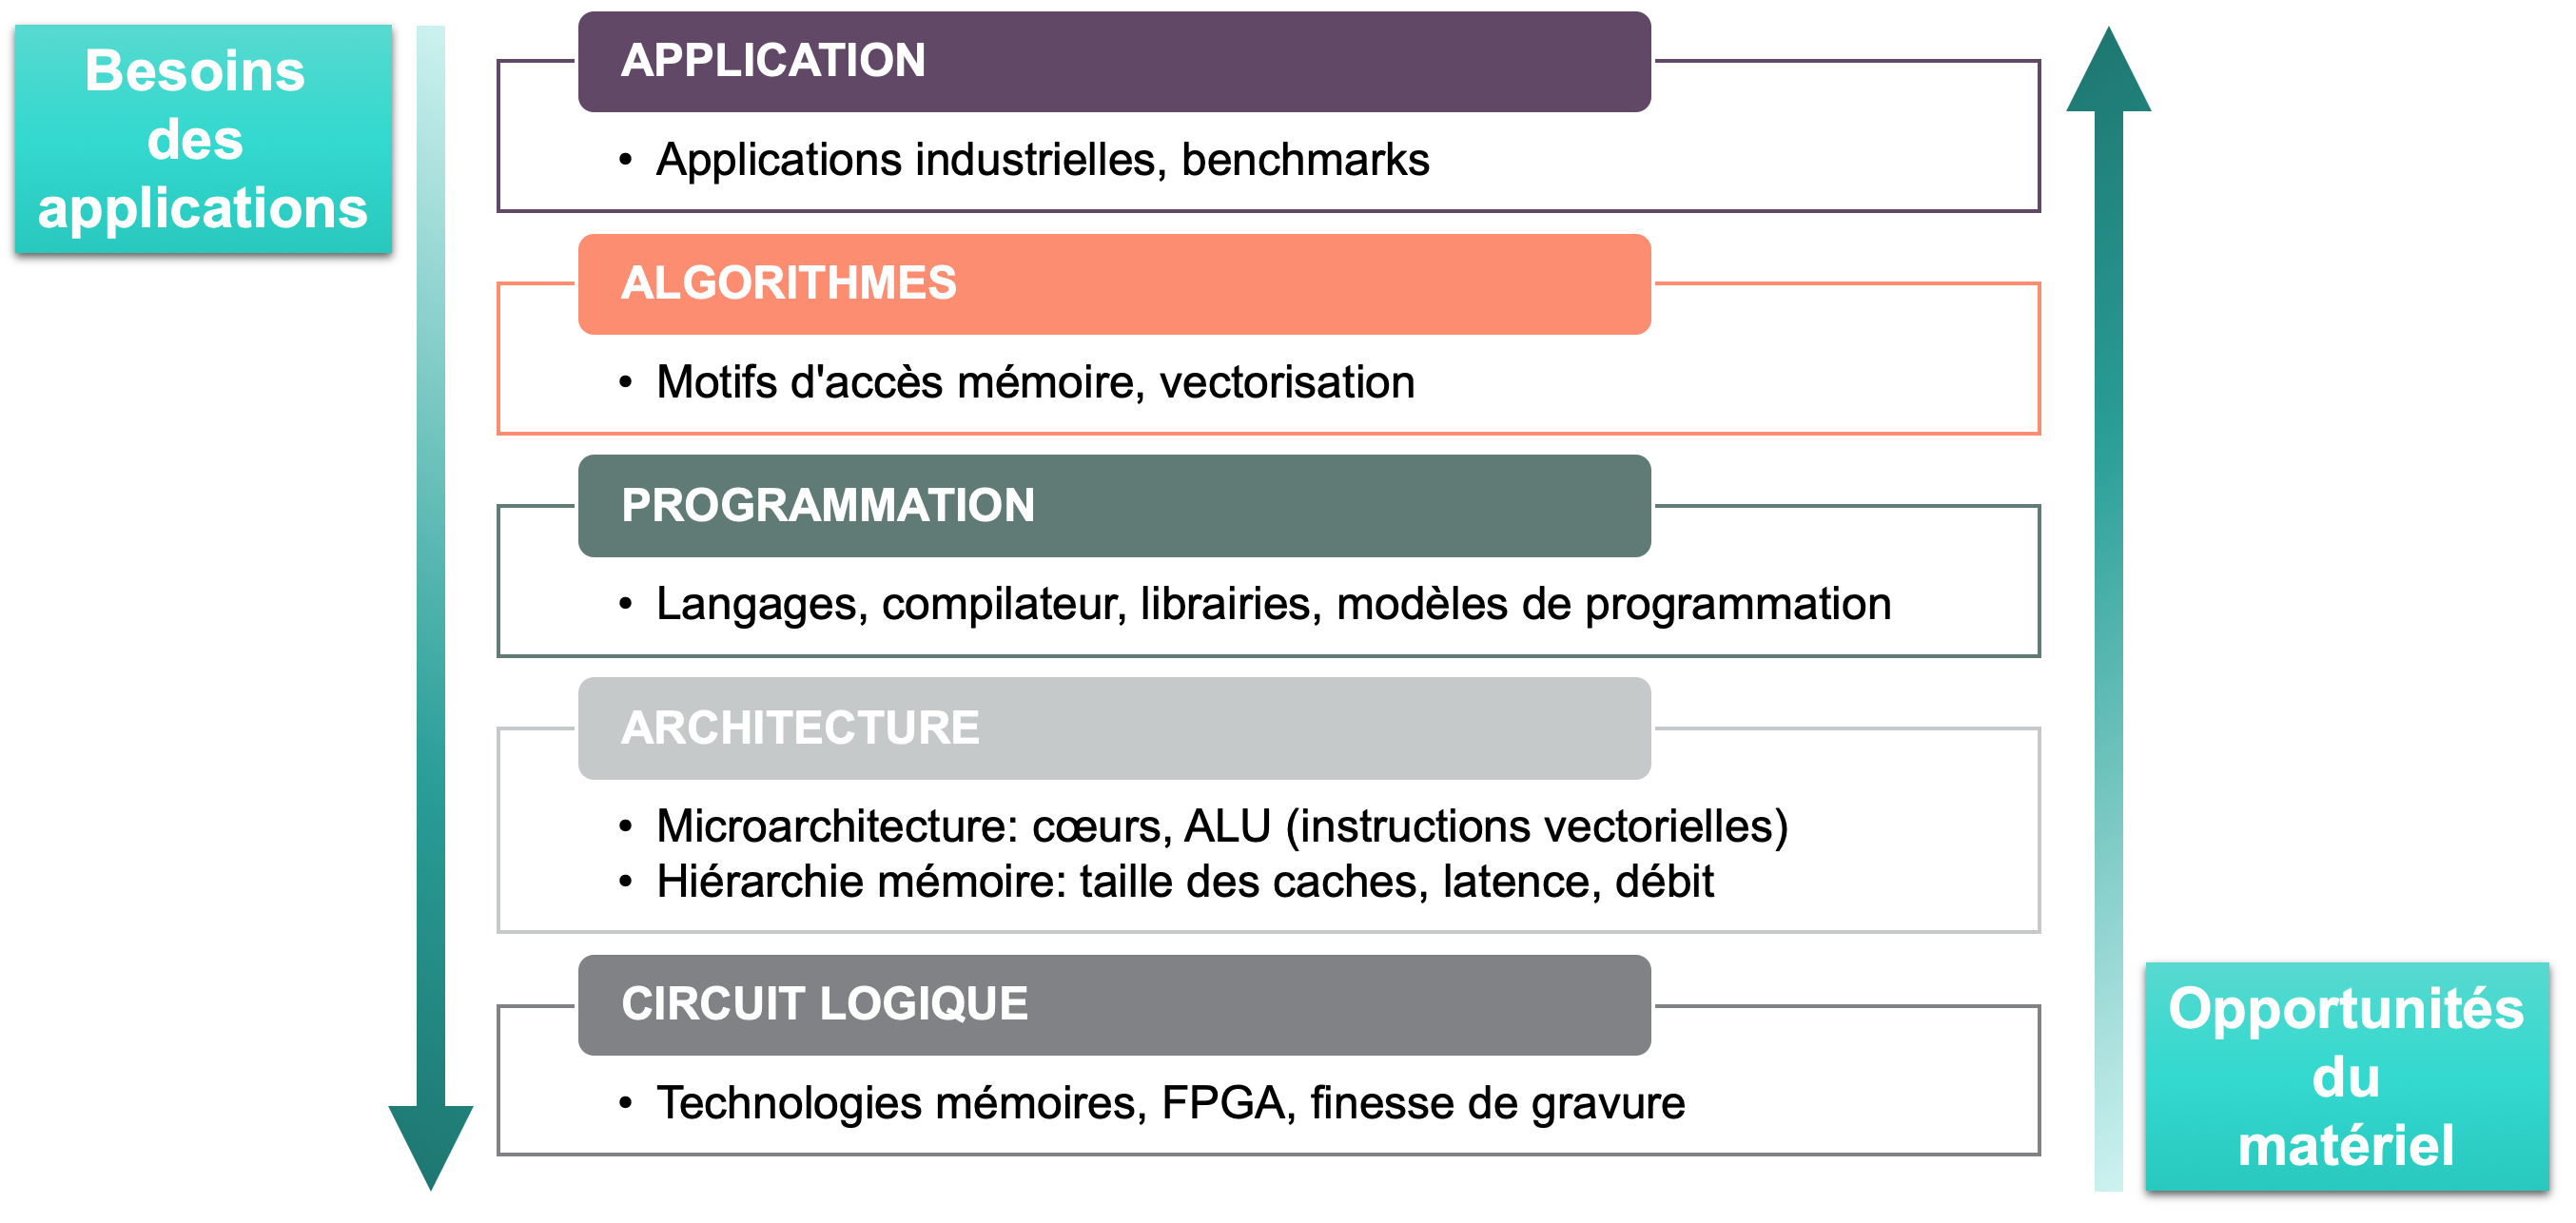
\includegraphics[width=14cm]{images/edl_co_design.png}
        \caption{\label{fig:edl_co_design} Processus de co-design.}
        \end{figure}
        
        Le développement en co-design suit un processus d'aller-retour entre la partie logicielle et la partie matérielle (voir \autoref{fig:edl_co_design}). Les utilisateurs de HPC (programmeurs, scientifiques) expriment les besoins de leurs applications aux constructeurs de matériels: débit mémoire, latence, scalabilité, puissance de calcul. Cette étape peut être difficile, car certaines applications comptent plusieurs millions de lignes de codes, et l'expression de leurs besoins est loin d'être triviale. Il peut alors être intéressant d'utiliser des applications plus simples se comportant comme les applications réelles (benchmarks, micro-benchmarks). 
        En étant conscients du besoin des applications, les fabricants peuvent développer des architectures adaptées. Pour cela, il est nécessaire d'utiliser toutes les avancées technologiques réalisées dans différents domaines (mémoire, interconnexion). Ensuite, les constructeurs peuvent communiquer aux développeurs certaines spécificités du matériel qui peuvent être exploitées par le logiciel (caractéristiques de la hiérarchie mémoire, instructions utilisables). Le principal frein de cette méthode est économique. Il faut que l'utilisation d'une architecture puisse bénéficier au maximum d'applications pour qu'un constructeur prenne la décision de la développer.
        
        Ces solutions pourront être développées pour accélérer certains algorithmes ou motifs de calcul \cite{asanovic2006landscape}: algèbre linéaire (matrices creuses ou denses), méthode spectrale (transformation de Fourier rapide), algorithmes de Monte-Carlo, graphe, programmation dynamique. Un exemple de co-design vise à adapter les unités de calcul aux besoins d'une l'application (instructions vectorielles, précision). Lorsque celles-ci ne nécessitent pas de réaliser des calculs avec une grande précision, il peut alors être intéressant d’utiliser des registres plus petits. L’étude \cite{Horowitz2014} montre que les opérations flottantes sur des registres plus petits consomment moins d’énergie: 0.03 pj pour une addition sur 8 bits contre 0.9 pj pour une addition sur 32 bits. De plus, le coût énergétique d’une multiplication évolue avec la taille ($n$) des registres utilisée ($O(n^2)$) ainsi que la latence ($O(n)$) \cite{Sze2017}. Enfin, le nombre de transistors nécessaires réduit avec la taille des registres ($36 \mu m^2$ contre $4184 \mu m^2$) pour des additionneurs de 8 et 32 bits \cite{Horowitz2014}. Cette technique a été utilisée par Google pour le développement de son ASIC en 2015. Le TPU est un ASIC optimisé pour réaliser la phase d'inférence des modèles d'apprentissage. Cette phase ne nécessite pas d'avoir autant de précision que la phase d'entraînement. Les ingénieurs ont donc développé le TPU en utilisant 65536 registres de 8 bits. Cette réduction d'un facteur 8 permet de réduire la consommation électrique et la taille des circuits par un facteur 6 \cite{Jouppi2017}. La latence de réponse, importante pour la phase d'inférence, est réduite entre 15 et 30 fois par rapport au GPU équivalent de l'époque (Nvidia K80).
            
          
            
            %Les architectures pourront ensuite être utilisées dans d'autres systèmes (ordinateurs personnels, téléphones). Ces méthodes sont déjà largement utilisées dans le domaine de la programmation embarquée, qui utilisent des processeurs (ou ASIC) prévus pour des tâches spécifiques. 
    
        %%%%%%%%%%%%%%%%%%%%%%%%%%%%%%%%%%%%%%%%%%%%%%%%%%%
        
    \subsubsection{Nouvelles architectures}\label{sec:new_soc}
    
        Pour répondre aux challenges exposés dans la section précédente, de nombreuses entreprises se lancent dans le développement de nouvelles architectures, qui peuvent être très différentes de celles que nous utilisons depuis 30 ans. En janvier 2018, une étude \cite{Metz2018} a dénombré 45 start-ups qui développaient des circuits spécialisés pour certaines applications d’intelligence artificielle: analyse de voix, conduite autonome\ldots Cinq  d’entre elles avaient alors levé plus de 100 millions de dollars d’investissement. Les derniers classements du Top500 ont vu l'apparition de supercalculateurs utilisant de nouveaux accélérateurs ou l'évolution d'ancienne. Par exemple, les GPU Nvidia utilisaient seulement de la mémoire GDDR5 sur les cartes des architectures Keppler. La génération suivante (Volta) a permis d'utiliser un interposeur en silicium connectant directement au processeur une mémoire HBM2. Ceci a permis de réduire les coûts énergétiques associés aux communications de 100 pj/bit à moins de 10 pj/bit. L'efficacité énergétique des supercalculateurs a ainsi pu être améliorée, passante de 6.7 à 14.1 GFLOPS/watt\footnotetext{Comparaison des classements du Top500 entre juin 2016 et 2017 des supercalculateurs Shoubu et Tsubame3.0}. En plus de nouvelles cartes GPU (Nvidia V100), deux nouveaux accélérateurs sont utilisés dans les supercalculateurs classés en tête du Green500: le PEZY-SC2 et le processeur ARM A64FX. Nous comparons les principales caractéristiques de ces architectures avec celle d'un processeur Intel moderne (génération Kaby Lake) dans le \autoref{tab:new_soc}.
        
                
        % Please add the following required packages to your document preamble:
        % \usepackage{graphicx}
        \begin{table}[]
        \centering
        \resizebox{\textwidth}{!}{%
        \begin{tabular}{|l|c|c|c|c|c|c|}
        \hline
         & \textbf{Coeurs/Thread} & \textbf{Freq. (GHz)} & \textbf{Débit mémoire (GB/s)} & \textbf{Perf. DP (TFLOPS)} & \textbf{TDP (Watt)} & \textbf{Eff. (GFLOPS/watt)} \\ \hline
        Intel Xeon 6246 & 12 / 24 & 3.30 & 140 (DRAM) & 1 & 165 & 6 \\ \hline
        Nvidia V100 & 5120 & 1.5 & 900 (HBM2) & 7.8 & 300 & 26 \\ \hline
        Pezy-SC2.2 & 2048 / 16384 & 1 & 2000 (DRAM + HBM2) & 4.1 & 180 & 23 \\ \hline
        Fujitsu A64FX & 48 & Non communiquée & 1000 (HBM2) & 2.7 & 180 & 15 \\ \hline
        \end{tabular}%
        }
        \caption{Caractéristiques et performances d'architectures utilisées dans les supercalculateurs les plus efficaces du Top500.}
        \label{tab:new_soc}
        \end{table}
                
        \textbf{Les architectures PEZY-SCx} sont des accélérateurs multicoeurs développés par la société PEZY.  Ils sont utilisés dans plusieurs supercalculateurs (ZettaScaler) construits au Japon. La dernière version, PEZY-SC2, a une surface six fois plus grande que le processeur Intel auquel il est généralement associé. La puce dispose de quatre canaux mémoires permettant d'atteindre une bande passante de 95.37 GB/s. En plus, l'accélérateur utilise une technologie sans fil (ThruChip Interface (TCI)) pour communiquer avec une mémoire 3D (voir \autoref{fig:edl_pezy_arch}). Chaque interface peut atteinte 500 GB/s pour un total de 2 TB/s. 
          
        \begin{figure}[t!]
            \centering
            \begin{subfigure}[t]{0.48\textwidth}
                \centering
                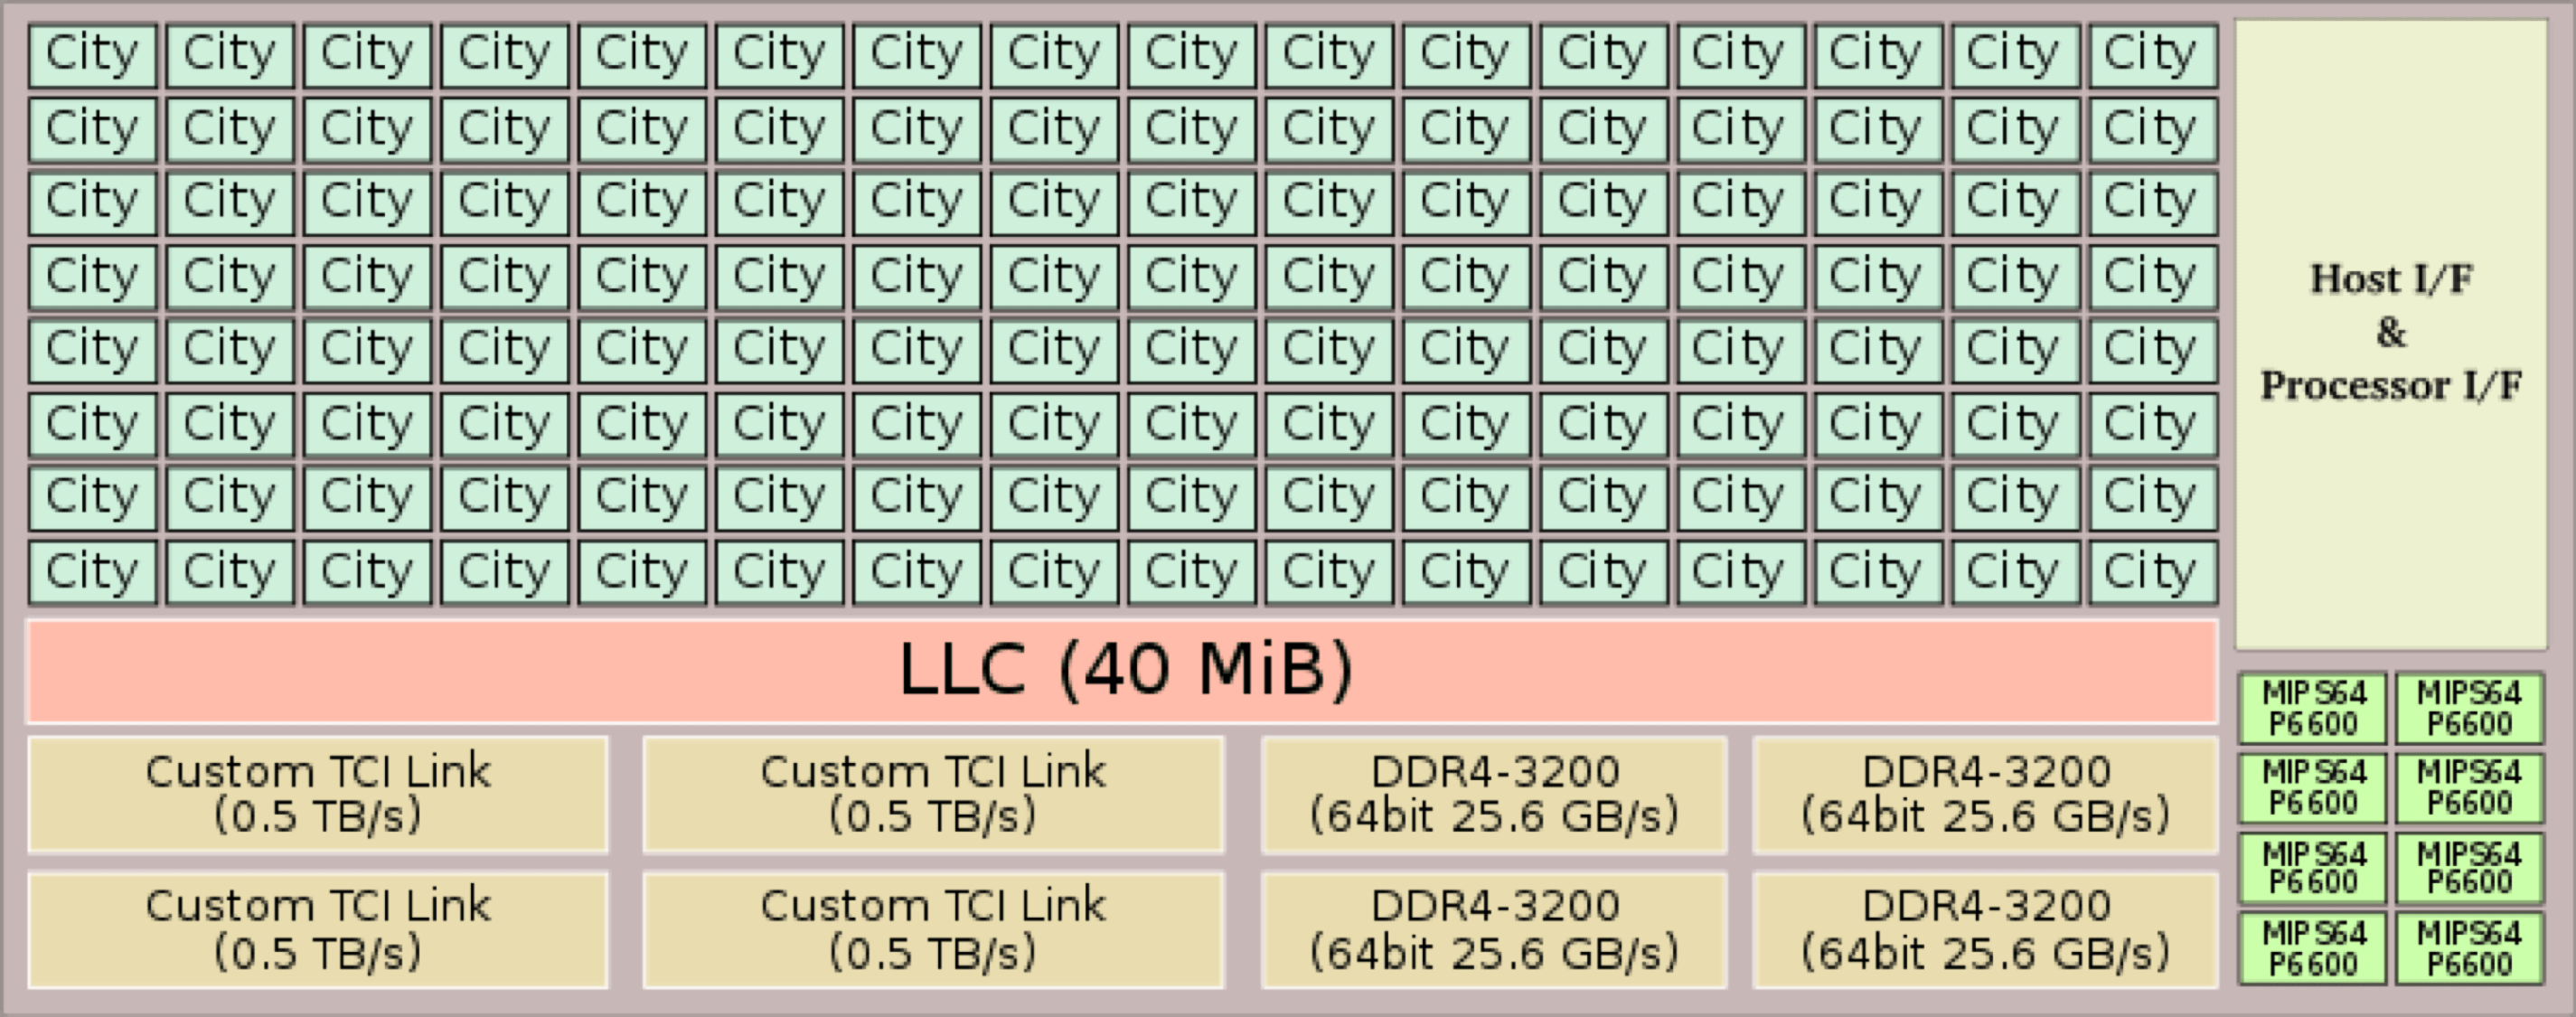
\includegraphics[width=\linewidth]{images/edl_pezy_arch.png}
                \caption{\label{fig:edl_pezy_arch}microarchitecture de l'accélérateur.}
            \end{subfigure}\hfill
            \begin{subfigure}[t]{0.48\textwidth}
                \centering
                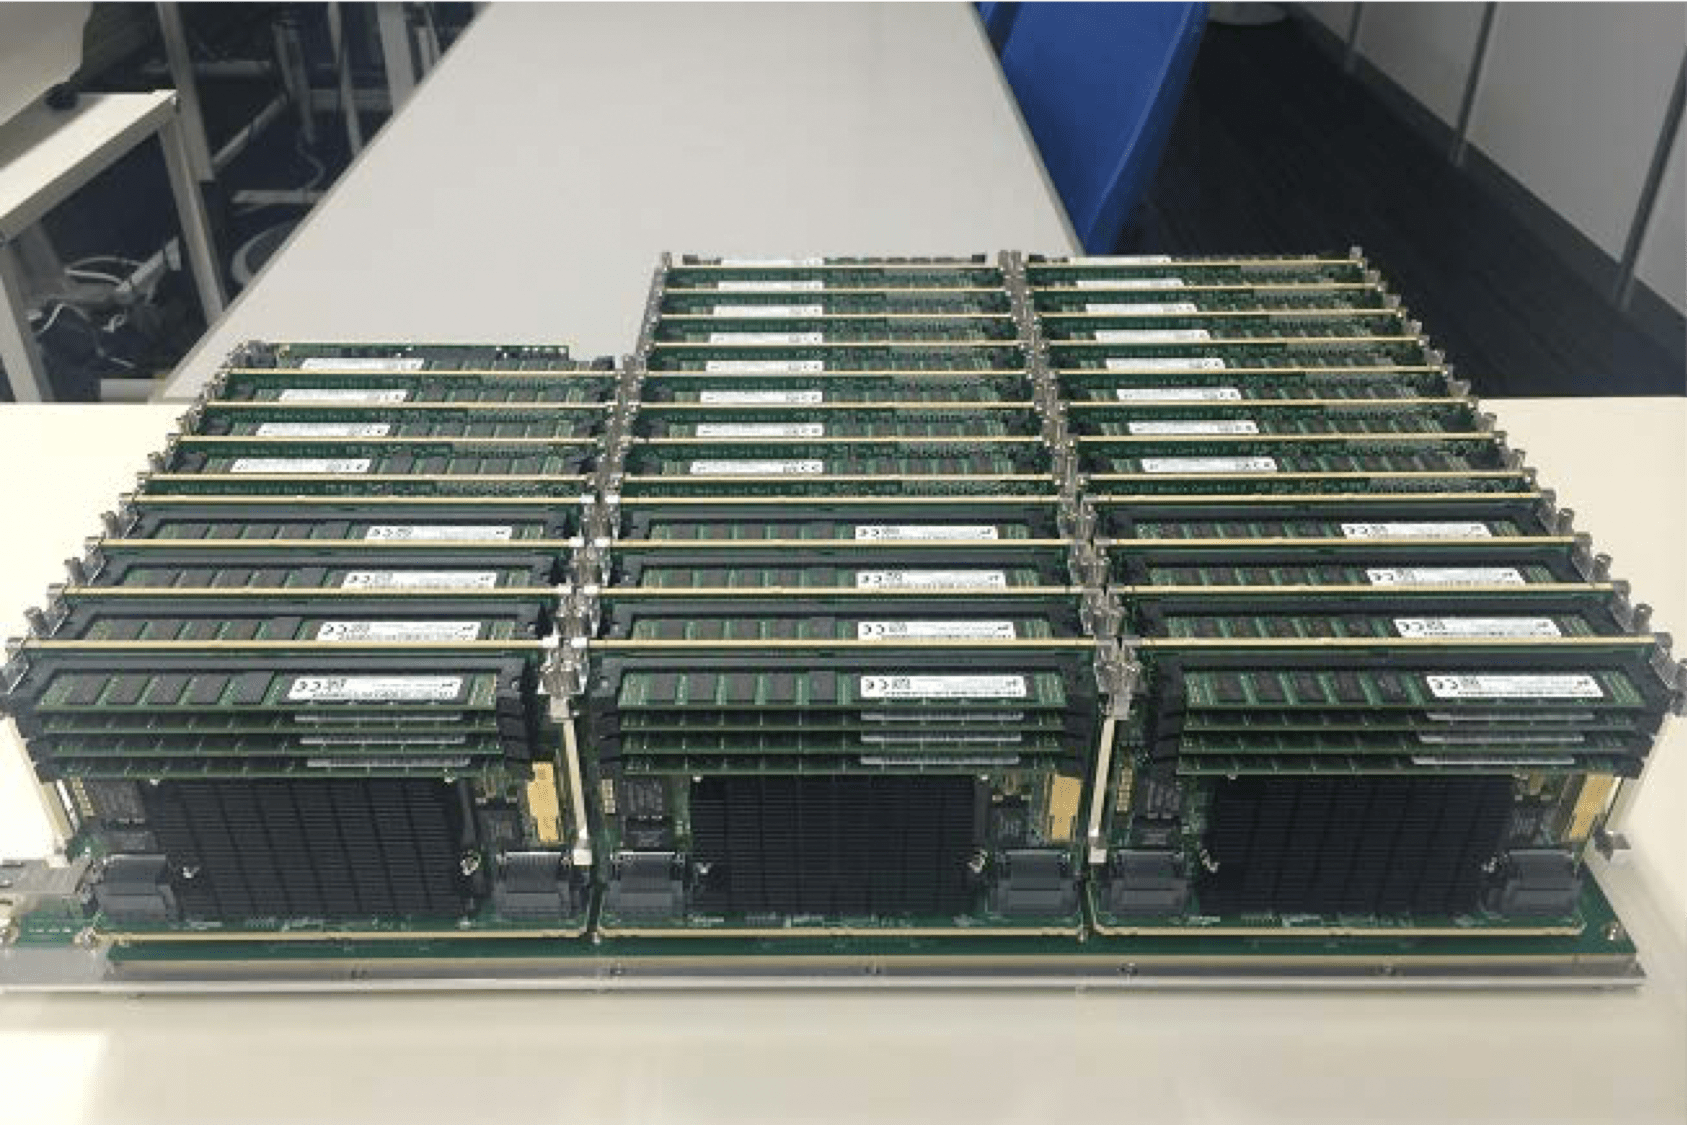
\includegraphics[width=\linewidth]{images/edl_pezzy_board.png}
                \caption{\label{fig:edl_pezzy_board}Plusieurs PEZY-SC2 peuvent être connectés sur un serveur.}
            \end{subfigure}
            \caption{\label{fig:pezy} Accélérateur PEZY-SC2 \cite{RyutaroHimenoToshikazuEbisuzaki2018}}
        \end{figure}
        
        \textbf{Le processeur ARM A64FX} développé par Fujitsu est le processeur équipant le premier supercalculateur classé au Green500. Il possède 48 coeurs capablent d'exécuter des instructions vectorielles de 512 bits. Il est doté de 32 GB de mémoire HBM2 permettant d'atteindre la performance de 2.7 TFLOPS ($10^{12}$ \gls{FLOPS}). Alors que le processeur A64FX n'est pas le plus efficace des 4 processeurs listés dans le \autoref{tab:new_soc}, il est pourtant utilisé dans le premier supercalculateur du Green500. En effet, nous remarquons que la puissance électrique d'une architecture ne suffit pas à déterminer l'efficacité énergétique d'une solution complète. Le reste de la plateforme doit lui aussi rentrer en compte (mémoire, utilisation du port PCI-E). La densité d'installation des architectures peut aussi avoir un impact (voir \autoref{fig:edl_pezzy_board}). Ainsi, malgré que le GPU Nvidia V100 soit le plus efficace, les solutions utilisant les processeurs ARM et PEZZY qui sont les mieux classés.
        
    \subsubsection{Hétérogénéité} \label{sec:edl_hpc_hetero}
        
        Avec la fin de la loi de Dennard et les premiers signes d'apparition du mur de l'énergie, les constructeurs ont été contraints de repenser la microarchitecture des processeurs. Les processeurs utilisés étaient alors désignés comme d'usage général (\textit{general purpose processor} (GPP)). Permettant d'exécuter tout type d'application, ces processeurs ne sont optimisés pour aucune d'entre elles. 
        La performance et l'efficacité énergétique sont les deux raisons qui ont poussé la communauté HPC à adopter cette technologie. L'évolution des langages et des libraires a permis de faciliter les développements d'application pour ces accélérateurs. En 2007, Nvidia publiait CUDA, un langage propriétaire permettant de programmer les cartes graphiques de la marque ainsi que des librairies de calculs mathématiques optimisées (CUBLAS, CUFFT). Ainsi, le nombre de supercalculateurs hétérogènes présents dans le Top500 n'a fait qu'augmenter ces dix dernières années pour atteindre près d'un supercalculateur sur trois en 2019 (voir \autoref{fig:edl_hetero_share}). À partir de 2010, les premiers clusters contenant des cartes graphiques apparaissent au classement du Top500 (voir le graphique \ref{fig:edl_gpu_top500}). Il faut attendre 2011 pour voir une réelle percée de cette technologie. En 2018, les GPUs étaient les principaux accélérateurs utilisés dans les supercalculateurs (93\% des plateformes hétérogènes du Top500 en 2018). 
        
        
        

       \begin{figure}[t!]
            \centering
            \begin{subfigure}[t]{0.58\textwidth}
                \centering
                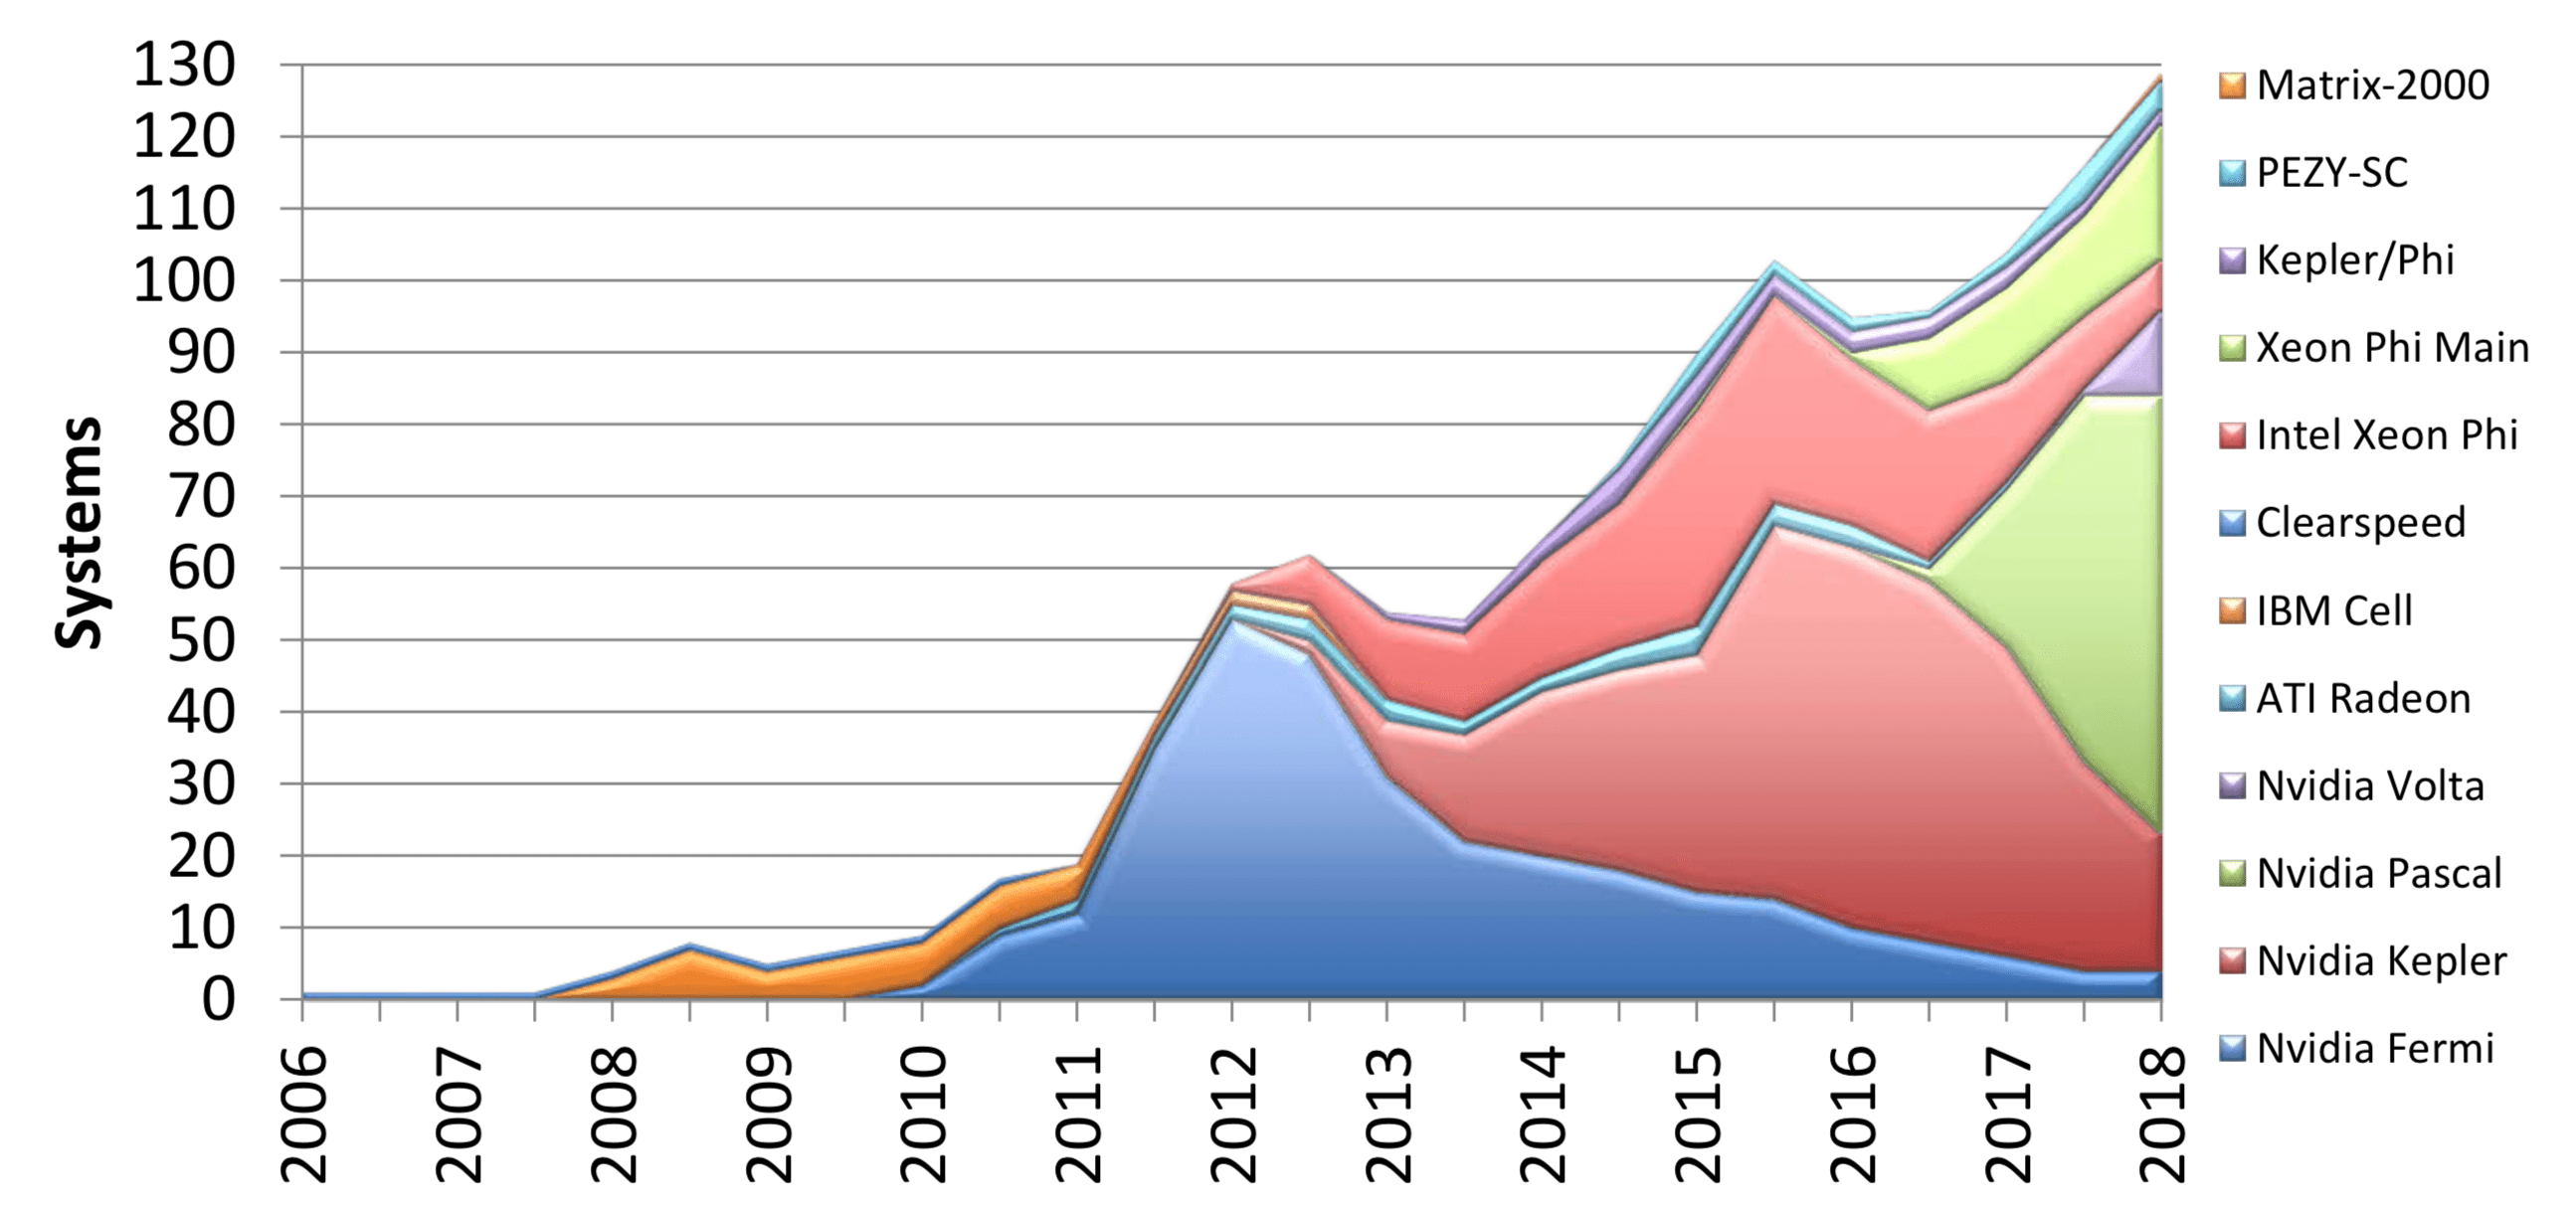
\includegraphics[width=\linewidth]{images/edl_gpu_top500.png}
                \caption{\label{fig:edl_gpu_top500} Évolution des différents types d'accélérateurs utilisés \cite{Strohmaier2018}.}
            \end{subfigure}\hfill
            \begin{subfigure}[t]{0.41\textwidth}
                \centering
                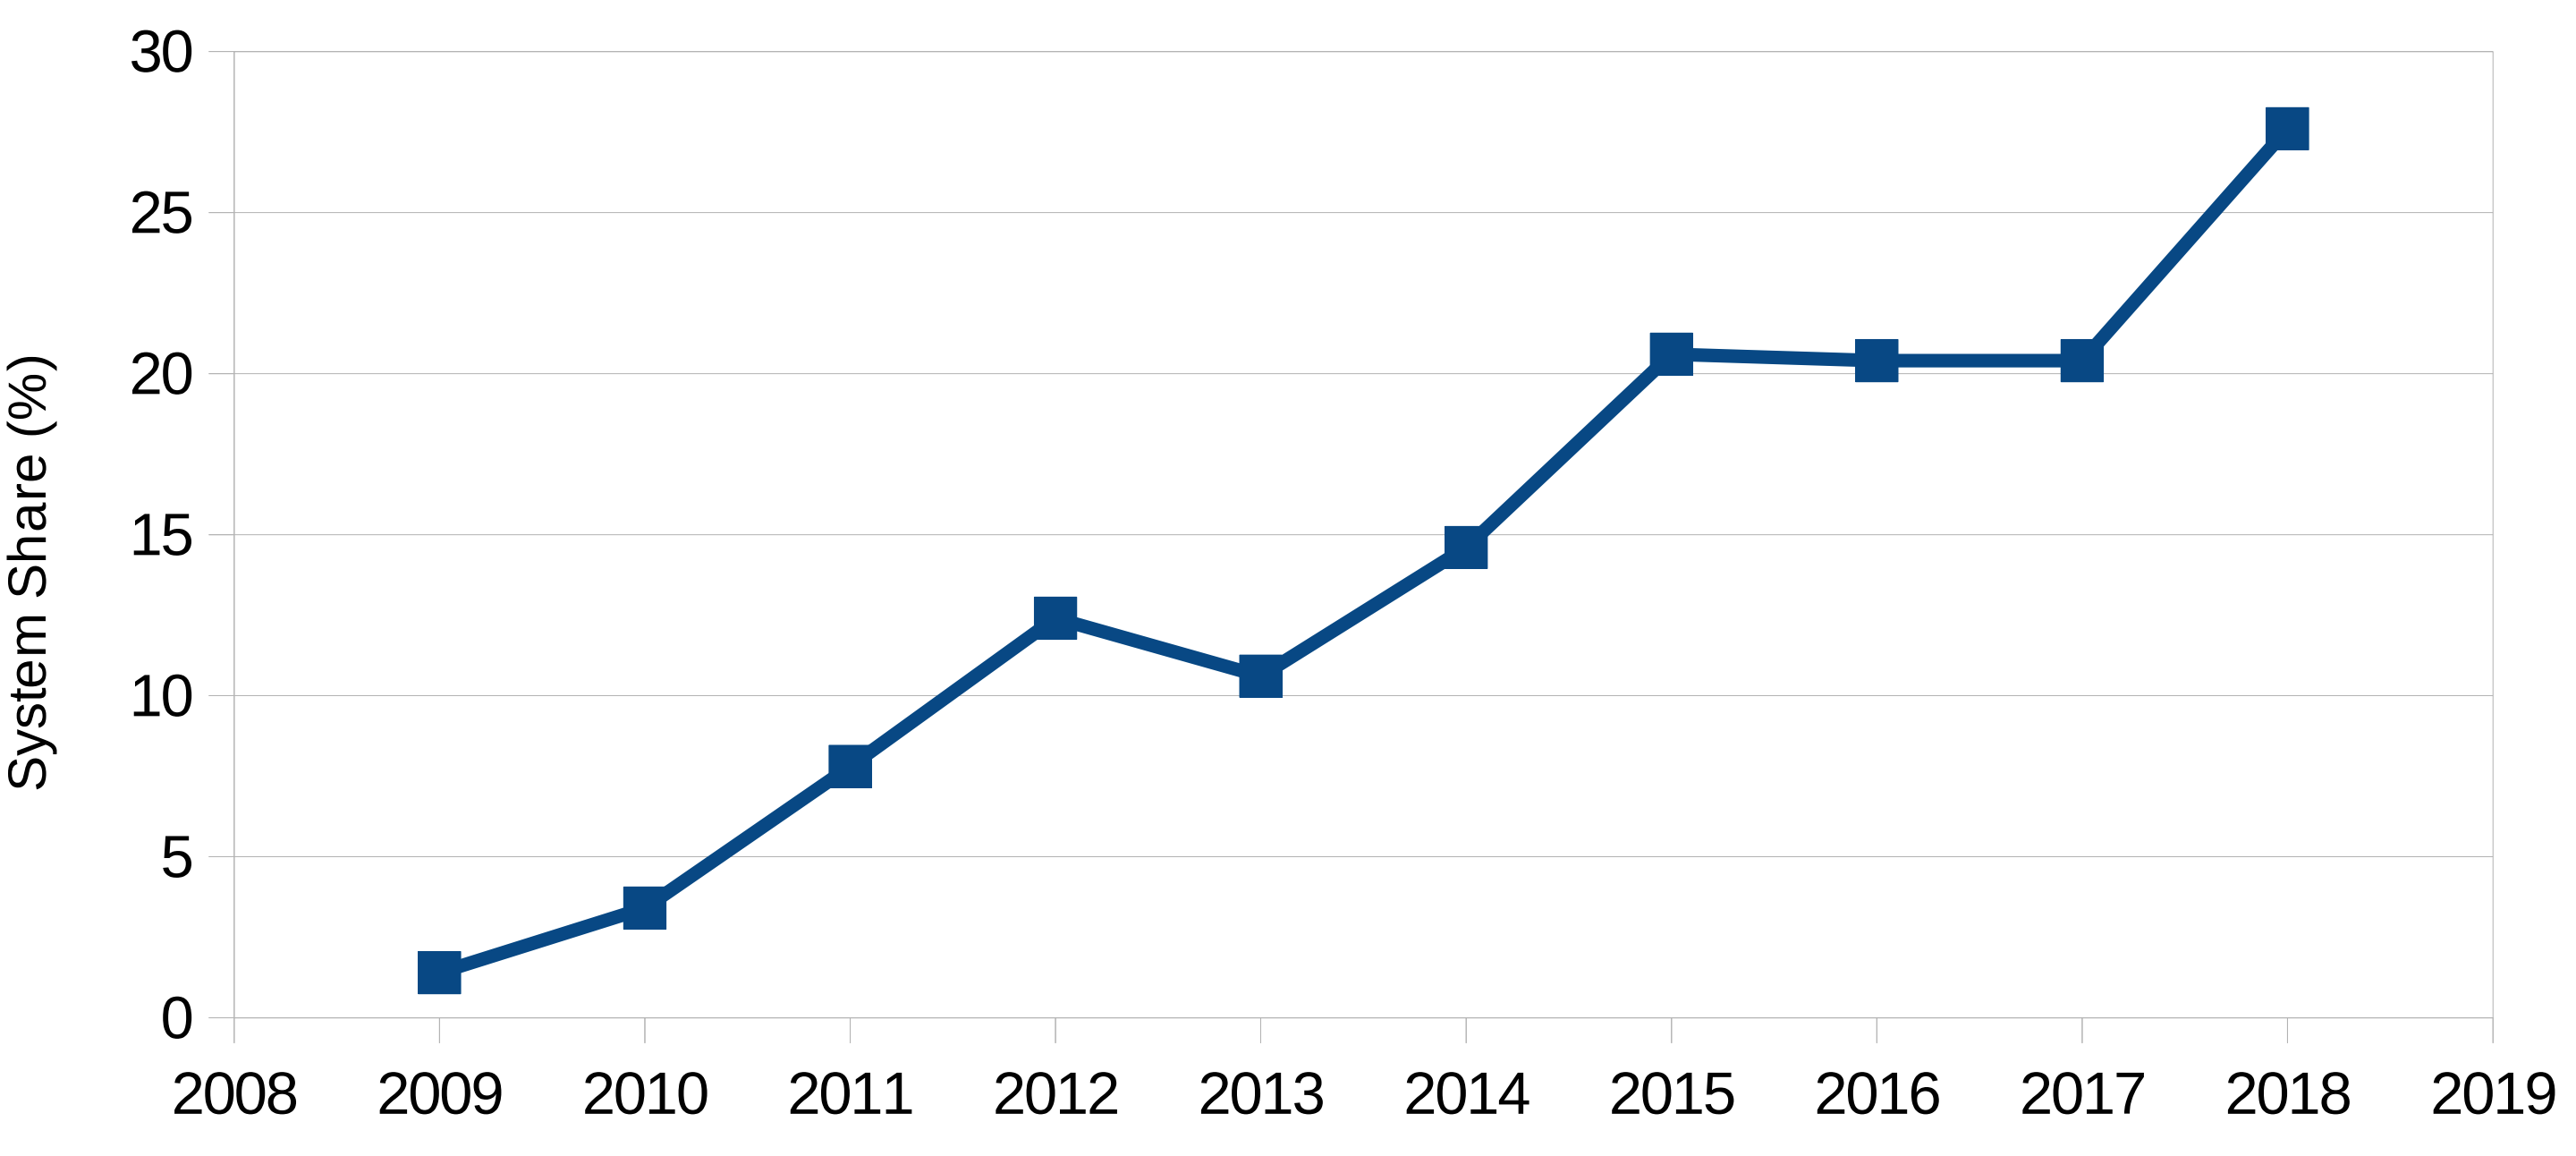
\includegraphics[width=\linewidth]{images/edl_hetero_share.png}
                \caption{\label{fig:edl_hetero_share} Évolution du pourcentage de supercalculateurs utilisant un accélérateur \cite{phdthesis}.}
            \end{subfigure}
            \caption{Évolution de l'utilisation d'accélérateurs dans les supercalculateurs.}
        \end{figure}
        
        
        En 2020, la majorité des supercalculateurs n'utilise cependant pas d'accélérateurs. En effet, les plateformes homogènes ont plusieurs avantages. La performance des processeurs GPP peut être suffisante pour une majorité d'applications. L'utilisation d'une seule famille de processeur facilite aussi la gestion du centre de calculs. Aussi, l'utilisation d'un processeur type x86 assure une stabilité à long terme, où l'utilisation de la génération suivante d'une architecture est similaire et ne nécessite généralement pas de grosse transformation de code. 
        
        D'un autre coté, utiliser des architectures hétérogènes peut présenter plusieurs difficultés. La première vient de la nécessité de transformer ou de reprogrammer les applications pouvant nécéssiter l'utilisation de langages  ou des modèles de programmation différents. Ces transformations demandent un gros investissement des programmeurs. D'autres difficultés concernent la gestion et l'utilisation des ressources. Les supercalculateurs sont utilisés pour exécuter différents types d'applications, avec différents besoins. Utiliser un seul type d'accélérateur ne sera pas efficace pour toutes les applications. La combinatoire engendrée par la disponibilité de plusieurs types d'accélérateurs, de capacité de mémoire différente complique l'obtention des performances optimales. La recherche des configurations optimales (compilateur, drapeaux de compilation, type d'accélérateur, taille de découpage des jeux de données, nombre de coeurs et fréquence utilisés) est alors difficile à réaliser manuellement. Pour explorer les différentes configurations, il peut alors être intéressant de se tourner vers des techniques d'autoréglage (\textit{auto-tuning}) \cite{datta2008stencil, hoste2008cole, mazouz2011performance, castro2015cere, popov:tel-01412638,  benkner_et_al:DR:2014:4423} 
        
        Une récente étude \cite{inproceedingsSCHC} conduite auprès de plusieurs industries montre que l'investissement nécessaire pour réaliser ces transformations est un frein majeur à l'adoption de ces architectures. La transformation du code est loin d'être évidente et varie en fonction des accélérateurs choisis (voir \autoref{fig:edl_many_techno}). Les langages, librairies et outils de programmation (debbuger, suivi de performance) sont moins avancés et robustes que ceux utilisés sur des architectures classiques. Les quatre entreprises interviewées \cite{inproceedingsSCHC} constatent le manque d'outils adaptés pour réaliser le travail du portage de code et de validation de performances. C'est une différence majeure entre l'industrie et le domaine de la recherche. Les applications industrielles sont plus complexes que celles utilisées comme démonstrateurs et il est souvent plus difficile d'atteindre les performances théoriques. Une entreprise témoignant dans l'étude \cite{inproceedingsSCHC} affirme que le manque d'expertise était le principal challenge pour le portage d'application. Ce constat est partagé par les autres entreprises présentées comme \textit{larges} et ayant les moyens d'embaucher de potentiels experts.
        
        Cependant, les pressions énergétiques et économiques obligeront les plus grands centres à se doter de plateformes hétérogènes malgré les difficultés associées. 
        
        \begin{figure}
        \center
        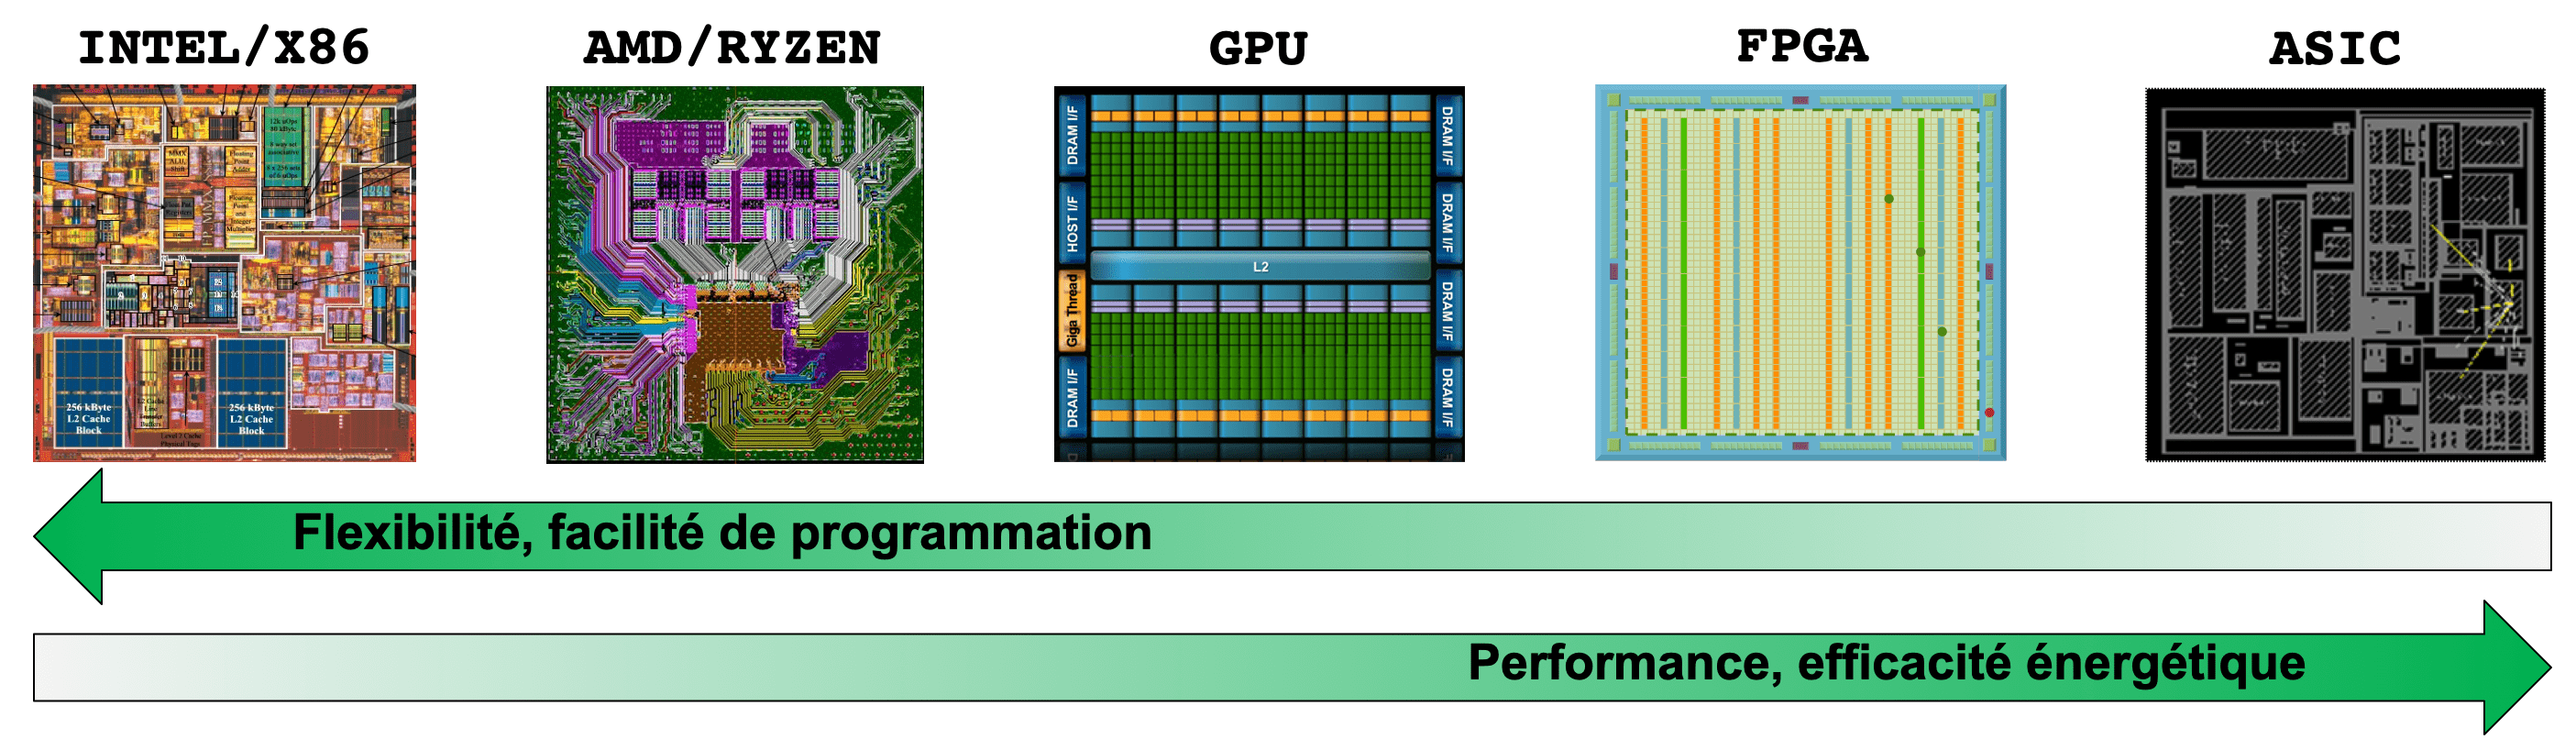
\includegraphics[width=17cm]{images/edl_many_techno.png}
        \caption{\label{fig:edl_many_techno} Différentes technologies sont disponibles, chacune ayant ses avantages et inconvénients.}
        \end{figure}
            
        Dans le projet \gls{exascale}, l'hétérogénéité ne viendra pas seulement de l'utilisation d'accélérateurs différents. Les architectures elles-mêmes seront développées à partir de différentes technologies, pour maximiser l'efficacité énergétique. Le co-design associé aux technologies photoniques va permettre le développement d'architectures ultra-optimisées permettant la construction d'une plateforme \gls{exascale} consommant entre 20 et 30 MW. Les puces des processeurs vont être adaptées à l'application pour minimiser les échanges de données (voir \autoref{fig:edl_hetero_chip}). Un même processeur pourra alors disposer de différents types de coeurs (complexe (x86), simple (GPU), FPGA) ayant des mémoires aux caractéristiques, elles aussi différentes (capacité, latence, débit, politique de remplacement, associativité).  Par exemple, une application d'apprentissage automatique peut avoir besoin pendant la phase d'entraînement de ressources similaires aux GPU. Dans une seconde phase (inférence), un autre module (FPGA, ASIC), directement accessible sur la puce, peut alors être utilisé. Ainsi, les données ne nécessitent par d’être transférés sur un autre serveur et peuvent être encore présentes dans la hiérarchie mémoire (mémoire 3D, SCM, DRAM).
        
          \begin{figure}
        \center
        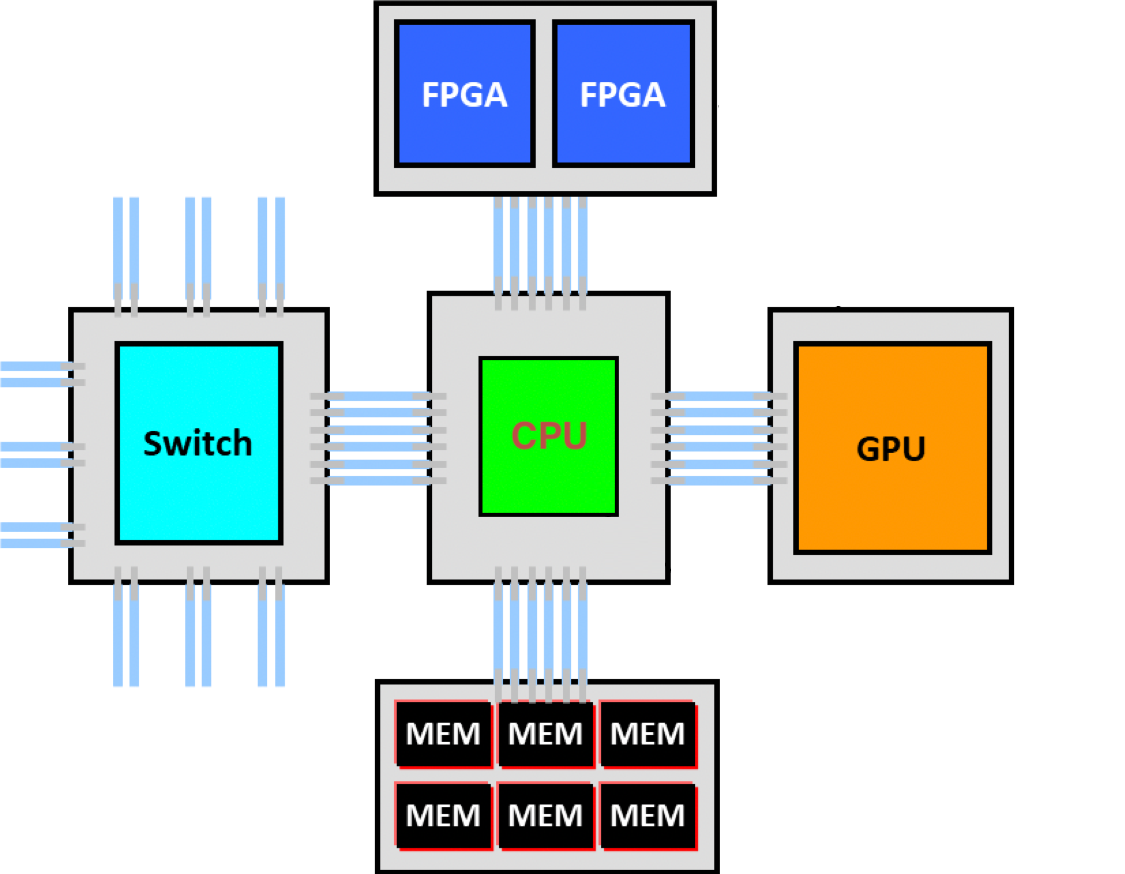
\includegraphics[width=9cm]{images/edl_hetero_chip.png}
        \caption{\label{fig:edl_hetero_chip}Développement de processeurs très hétérogènes possédant différentes technologies sur la même puce communiquant par photonique \cite{Bergman2018}.}
        \end{figure}
            
      

      
%%%%%%%%%%%%%%%%%%%%%%%%%%%%%%%%%%%%%%%%%%%%%%%%%%%%%%%%%%%%%%%%%%%%%%%%%%%%%%%%%%%%%%%%%%%%%%%%%%%%%%%%%%%%%%%%%%%%%
%%%%%%%%%%%%%%%%%%%%%%%%%%%%%%%%%%%%%%%%%%%%%%%%%%%%%%%%%%%%%%%%%%%%%%%%%%%%%%%%%%%%%%%%%%%%%%%%%%%%%%%%%%%%%%%%%%%%%
%%%%%%%%%%%%%%%%%%%%%%%%%%%%%%%%%%%%%%%%%%%%%%%%%%%%%%%%%%%%%%%%%%%%%%%%%%%%%%%%%%%%%%%%%%%%%%%%%%%%%%%%%%%%%%%%%%%%%
%%%%%%%%%%%%%%%%%%%%%%%%%%%%%%%%%%%%%%%%%%%%%%%%%%%%%%%%%%%%%%%%%%%%%%%%%%%%%%%%%%%%%%%%%%%%%%%%%%%%%%%%%%%%%%%%%%%%%
%%%%%%%%%%%%%%%%%%%%%%%%%%%%%%%%%%%%%%%%%%%%%%%%%%%%%%%%%%%%%%%%%%%%%%%%%%%%%%%%%%%%%%%%%%%%%%%%%%%%%%%%%%%%%%%%%%%%%


\subsection{Gen-Z}\label{sec:gen_z}
%%%%%%%%%%%%%%%%%%%%%%%%%%%%%%%%%%%%%%%%%%%%%%%%%%
    
    Cette section est consacrée à la présentation d'un nouveau protocole de communication nommé Gen-Z. Pour cela, nous résumons les principales motivations de la nécessité d'utiliser une telle technologie. Nous présentons ensuite les principales caractéristiques et les avantages du protocole. Enfin, nous discutons de l'opportunité apportée par Gen-Z pour repenser fondamentalement l'architecture de nos plateformes.
        
    \subsubsection{Motivations}
            %%%%%%%%%%%%%%%%%%%%%%%%%%%%%%%%%%%%%%%%%%%%%%%%%%%%%%%%%%%%%%

        % EXPLOSION
        Le tsunami de données générées présenté dans la \autoref{sec:challenges} nécessite de repenser la façon dont nous les traitons. Actuellement ces données sont envoyées aux centres de calculs pour être analysés. Le volume de données générées dans les prochaines années nous empêchera de poursuivre cette méthode. Une voiture connectée génère par exemple entre 2 et 5 terabytes de données chaque jour. Le coût des technologies et des infrastructures nécessaire pour les transférer vers les centres de données serait alors trop élevé. De plus, la conduite autonome comme d'autres applications (villes connectées) nécessite d'avoir des réponses rapides. La seule solution viable est alors de les traiter le plus proche possible de leur zone de création. Seule une partie d'entre elles sera alors remontée aux centres de calculs pour l'archivage ou améliorer l'apprentissage des réseaux de neurones.
        
        %securité
        Les voitures et les objets connectés produisent des données sensibles, et la nécessité d'utiliser des plateformes de traitement sécurisé est primordiale. Chaque composant des solutions est une source d’attaque potentielle: capteurs, processeurs, mémoires, réseaux. Les dégâts potentiels d'une attaque sur ces sites ultra-connectés pourraient alors être catastrophiques (attaque de la signalisation routière, de voitures connectées ou d'un système de refroidissement d'une centrale nucléaire).
    
        % HETERO
        Concernant le domaine du HPC, nous avons étudié dans les sections précédentes que de nombreuses technologies (mémoires, processeurs, accélérateurs) étaient en développement. Ces nouvelles architectures sont produites par différents constructeurs. Les architectures actuelles ont été développées pour un nombre limité de technologies (mémoire DRAM, processeur x86 ou ARM, extension PCIe). La principale difficulté pour leur utilisation viendra de leur compatibilité. 
        
       
                
    \subsubsection{Limites des architectures actuelles}
        %%%%%%%%%%%%%%%%%%%%%%%%%%%%%%%%%%%%%%%%%%%%%%%%%%%%%%%%%%%%%%
        Malgré l'évolution des accélérateurs et l'utilisation de nouvelles technologies mémoires, les architectures actuelles ne pourront pas évoluer indéfiniment et ont déjà montré leurs limites. La \autoref{fig:edl_genz_evo_memoire}, représente l'évolution des différentes caractéristiques liées aux bus de communication d'un processeur ainsi que l'évolution du nombre de coeurs disponibles. Nous constatons que l'évolution du nombre de coeurs a évolué plus rapidement que celle des performances du système mémoire. En effet, lorsque le nombre de canaux mémoires a été multiplié par 2 (passant de 4 à 6, puis à 8 canaux) le nombre de coeurs a été multiplié par un facteur 8.  Le débit du bus mémoire (courbe violette) et du bus PCIe (courbe rouge) disponible par coeur a donc diminué. La majorité des broches du processeur sont déjà utilisées par les canaux mémoires et il sera très difficile d'en allouer plus. 
        
            \begin{figure}
            \center
            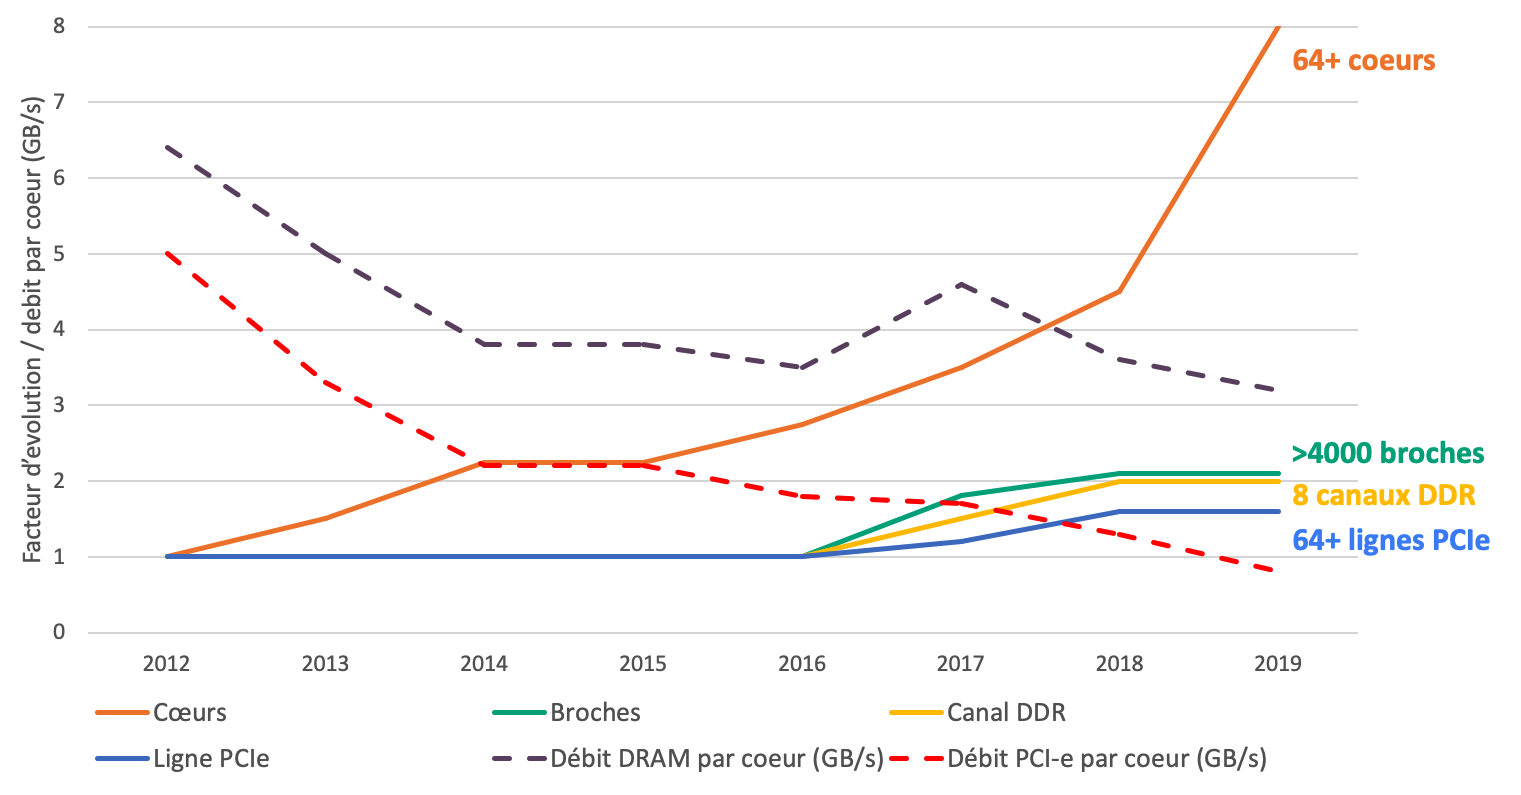
\includegraphics[width=14cm]{images/edl_genz_evo_memoire.png}
            \caption{\label{fig:edl_genz_evo_memoire} Évolution annuelle des caractéristiques principales des architectures (nombre de coeur, débit mémoire) et leur impact sur les débits disponibles par coeur.}
            \end{figure}
            
        
        %PLace
        De plus, le manque d'espace disponible sur la carte mère nous oblige à développer une solution permettant d'augmenter les débits de plusieurs facteurs avec les canaux actuellement utilisés. 
        L'espace disponible autour du processeur pour ajouter des emplacements mémoires est aussi de plus en plus limité. Les plus grosses configurations actuelles peuvent atteindre jusqu'à 1.5 TB de mémoire, insuffisant pour traiter les jeux de données envisagés.
    
        % lock step &
        Avec le modèle actuel, l'évolution des mémoires ou des processeurs est verrouillée. La nécessité que l'un soit compatible avec l'autre oblige les deux parties à évoluer de manière synchronisée. Par exemple, avant de pouvoir utiliser des mémoires DDR5, il faut que les processeurs la supportant soient développés. Cette dépendance est un frein à l'évolution.
        
        %SCM
        Le développement des mémoires SCM permettra à terme d'obtenir des performances proches de la DRAM. Cependant, elles ne permettront pas d'augmenter les débits mémoires de plusieurs facteurs. En effet, ces mémoires sont installées sous forme de DIMM (NVDIMM voir \autoref{sec:nvdimm}) ou sous forme d'extension de carte PCI (comme les mémoires Intel Optane). Ces deux emplacements ont les mêmes restrictions de performances dues aux bus utilisés (PCI et mémoire). De plus, l'utilisation d'extension PCI à ses limites, car ce bus ne supporte pas la cohérence de cache des mémoires associées (contrairement au bus mémoire).

        %Protocol Babel
        Un autre défaut des architectures actuelles impactant la performance des applications concerne la multiplicité des protocoles utilisés: DDR, PCIe, infiniband, Ethernet, sata (voir \autoref{fig:edl_genz_babel}). L'utilisation de différents protocoles à un coût, impactant la latence, le débit et l'énergie consommée pour chaque transfert. Pour développer une plateforme exascale efficace, il est donc nécessaire de revoir l'utilisation de ces protocoles.
            
           
        
   
        %%%%%%%%%%%%%%%%%%%%%%%%%%%%%%%%%%%%%%%%%%%%%%%%%%%%%%%%%%%%%%
        %%%%%%%%%%% GEN _ Z %%%%%%%%%
        %%%%%%%%%%%%%%%%%%%%%%%%%%%%%%%%%%%%%%%%%%%%%%%%%%%%%%%%%%%%%%
    
    \subsubsection{Gen-Z.}
        
    % DEFINITION
        Gen-Z est un protocole universel d'interconnexion, de puce à puce, permettant les échanges entre composants informatiques au travers de communications à sémantique en mémoire. Gen-Z est dit universel, car il permet de connecter différentes architectures (CPU, GPU, FPGA) ainsi que différents médias (mémoire, stockage, archive) à travers un unique protocole (voir \autoref{fig:edl_genz_overview}). Ces communications (asynchrones) peuvent être locales (entre les composants d'un même serveur), ou bien externes (entre deux serveurs). 


       \begin{figure}[t!]
            \centering
            \begin{subfigure}[t]{0.49\textwidth}
                \centering
                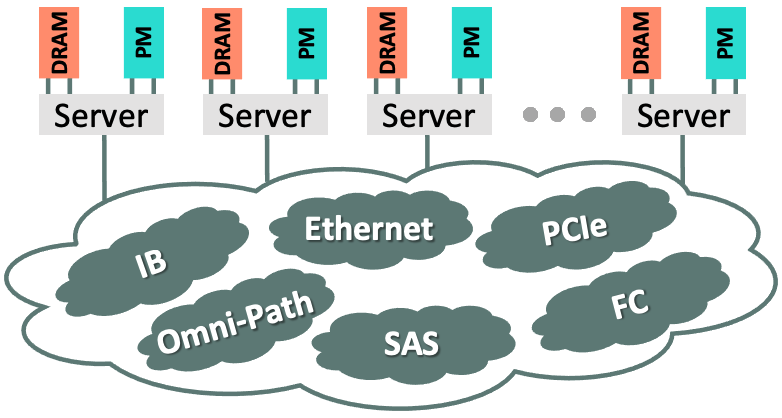
\includegraphics[width=\linewidth]{images/edl_genz_babel.png}
                \caption{\label{fig:edl_genz_babel} De nombreux protocoles sont impliqués lors d'une communication.}
            \end{subfigure}\hfill
            \begin{subfigure}[t]{0.49\textwidth}
                \centering
                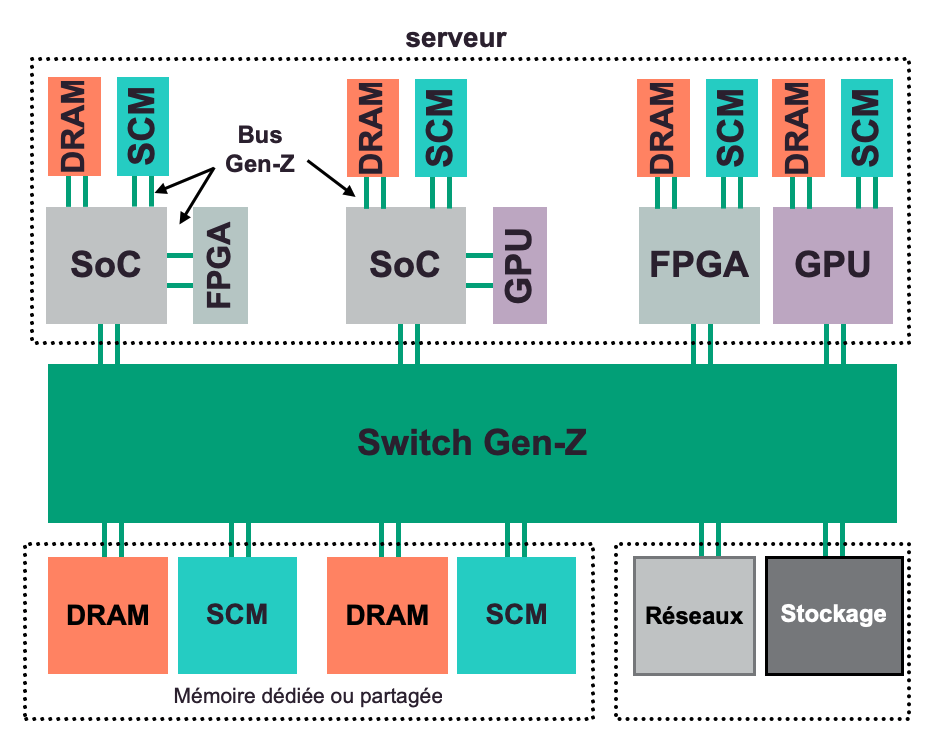
\includegraphics[width=\linewidth]{images/edl_genz_overview.png}
                \caption{\label{fig:edl_genz_overview} Le protocole Gen-Z permet d'interconnecter tous les composants d'une plateforme.}
            \end{subfigure}
            \caption{\label{fig:edl_genz_babel_topo} Gen-Z permet d'utiliser un unique protocole pour la totalité des communications.}
        \end{figure}
        
        
        Lancé en 2016, il est développé par un consortium qui compte aujourd'hui plus de 70 membres\footnotetext{Liste des membres du consortium Gen-Z - \url{https://genzconsortium.org/about-us/membership/members/}}, dont les plus grandes entreprises du domaine informatique: AMD, ARM, Cisco, Dell, Google, HP, HPE, Micron, Microsoft, Redhat, Samsung\ldots Il est important de noter l'absence de deux constructeurs majeurs (Intel et Nvidia) qui ont rejoint un deuxième consortium pour le développement d'un second protocole nommé CXL\footnotetext{Compute Express Link - \url{https://www.computeexpresslink.org/}}. Le développement de CXL est moins avancé que celui de Gen-Z.
        
        Ce protocole a été développé pour répondre aux nombreux challenges posés par l'utilisation des objets connectés et la nécessité de traiter des grands jeux de données. Gen-Z permet d'adresser un espace mémoire $2^{92}$ Byte (soit 4096 yottabytes, soit mille fois plus grands que notre espace numérique actuel) et d’interconnecter 16 millions d'objets. Ces objets pouvant être des composants d'un serveur (mémoire, processeur, accélérateurs) ou des objets connectés plus complexes.
            
    
    % SEMANTIQUE MEMOIRE

        \paragraph{Sémantique mémoire.} 
            L'avantage de Gen-Z est d'utiliser des communications à sémantique mémoire. Tous les composants sont considérés comme des modules mémoires et peuvent être accédé grâce à des instructions \textit{load/store}. Il est ainsi possible d'adresser les mémoires SCM par byte et non plus par bloc (héritage dû aux disques optiques). En réduisant la complexité des instructions, le processeur et le système d'exploitation ne sont pas impliqués dans leur exécution, libérant des ressources pour l'exécution d'autres instructions. Gen-Z propose d'autres instructions permettant de réaliser des opérations plus complexes telles que les opérations atomiques (comparaison, addition), des interruptions ou encore de gérer la cohérence des caches.
        
            Comme exposé en présentation de cette section, les évolutions technologiques des différentes parties d'une architecture sont dépendantes les unes des autres. Gen-Z permet de supprimer ce verrou. La \autoref{fig:edl_genz_bus_evo} présente comment les processeurs et les mémoires vont utiliser les interfaces Gen-Z pour être indépendantes. Le processeur et la mémoire auront une interface Gen-Z et l'évolution d'une partie ne nécessitera pas de changement de l'autre. De plus, en spécifiant un protocole universel, Gen-Z assure l'interopérabilité entre tout type de composant qui possède une interface (CPU, FPGA, GPU, DSP, I/O, mémoires).

            \begin{figure}[t!]
                \centering
                \begin{subfigure}[t]{0.49\textwidth}
                    \centering
                    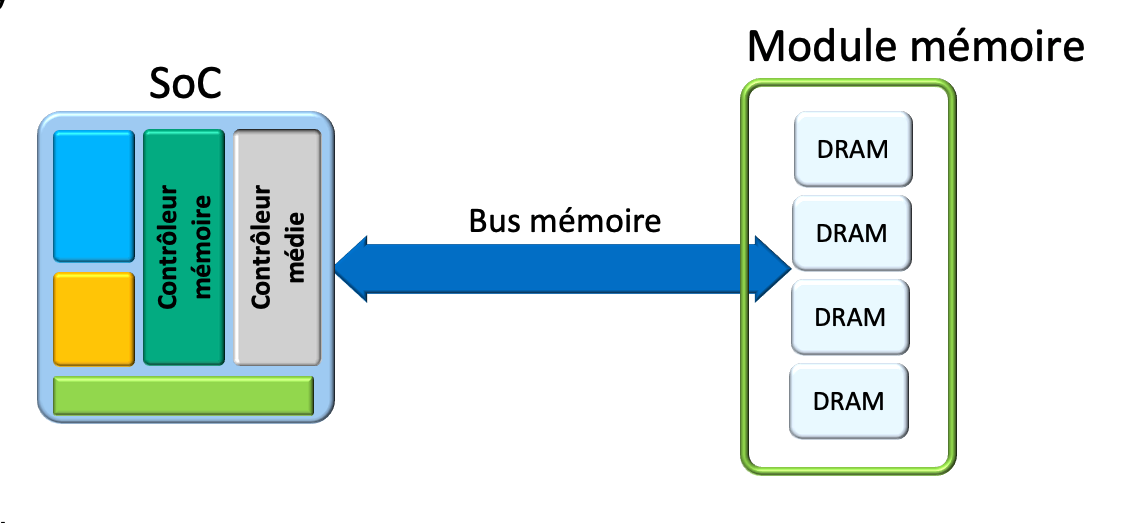
\includegraphics[width=\linewidth]{images/edl_genz_current_bus.png}
                    \caption{\label{fig:edl_genz_current_bus} Actuellement les technologies mémoires et celles des processeurs sont liées.}
                \end{subfigure}\hfill
                \begin{subfigure}[t]{0.49\textwidth}
                    \centering
                    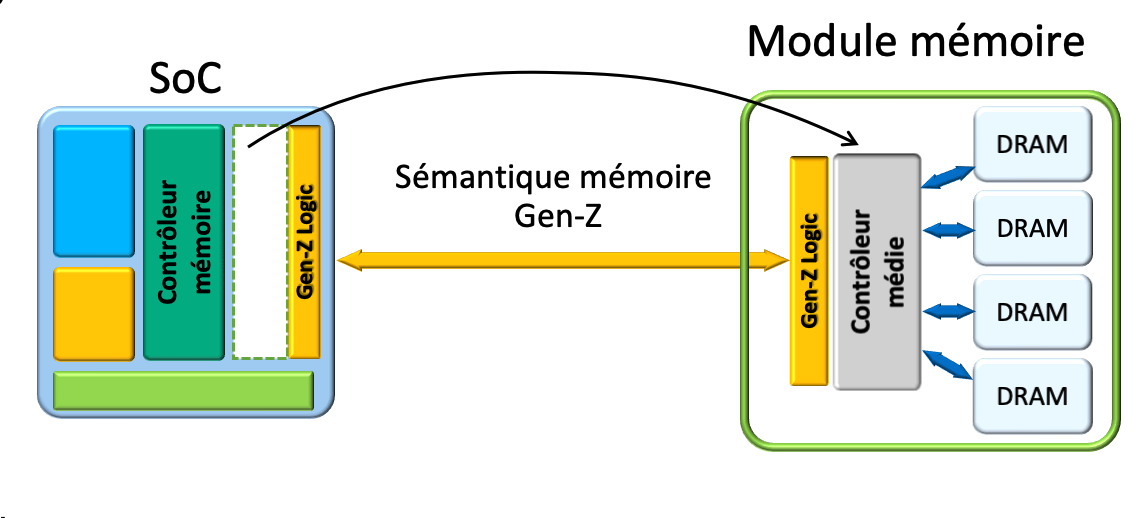
\includegraphics[width=\linewidth]{images/edl_genz_new_bus.png}
                    \caption{\label{fig:edl_genz_new_bus} Avec Gen-Z, chaque module aura sa propre interface.}
                \end{subfigure}
                \caption{\label{fig:edl_genz_bus_evo} Déverrouiller l'évolution technologique grâce à Gen-Z.}
            \end{figure}


    \paragraph{Latence et débit.}

        %Latence
        Le protocole Gen-Z permet d'améliorer les performances du système d'interconnexion et apporte aussi de nouvelles fonctionnalités permettant de repenser l'architecture des plateformes. La réduction du nombre de protocoles et des différentes couches impliquées dans le transfert des données (système de fichier, tampon I/O, drivers) permet de réduire les latences des accès. Les spécifications actuelles permettraient de réduire le nombre d'instructions de 25000 à 3 pour réaliser pour un transfert d'une donnée localisée sur un disque. En utilisant des technologies SCM, les latences d'accès entre un processeur et une mémoire située sur un autre serveur seraient alors proches de celles d'un accès à la mémoire DRAM locale (inférieur à 250 ns).
     
        %BANDE PASSANTE    
        Gen-Z permet d'atteindre des débits mémoires supérieurs à ceux des bus mémoires actuels. En fonction des technologies et du nombre de broches utilisées, les débits mémoires d'une architecture Gen-Z peuvent atteindre 1.7 TB/s. Ces performances sont possibles grâce au débit atteignable pour chaque broche du processeur utilisée. Il sera donc possible d'atteindre des débits mémoires 10 fois supérieurs avec la moitié de broches permettant de développer des processeurs moins coûteux. 
        % À titre de comparaison, la mémoire DDR5 permet d'atteindre 0.55 GB/s par broche.
        
            
            
            

    \paragraph{Topologie}

        Gen-Z supporte nativement différentes topologies (P2P, mesh, Torus) pour réaliser la connexion entre les composants, mais aussi entre les serveurs (voir \autoref{fig:edl_genz_topo}). Ces topologies permettent d'implémenter des réseaux multi chemins (\textit{multipath}) et de gérer le contrôle de congestion. Si un lien entre deux composants est cassé, le protocole s'adapte automatiquement en passant par d'autres chemins disponibles. Les différents composants peuvent alors servir de relais pour transmettre les paquets. Aujourd'hui lorsqu'un serveur tombe en panne, les données présentes dessus sont perdues, et les applications doivent être relancées. Gen-Z et les SCM permettront d'assurer une connexion permanente aux différents modules avec l'utilisation de la topologie HyperX \cite{Ahn2009} (voir \autoref{fig:edl_photo_hyperX}),  qui permet de joindre n'importe quel serveur avec trois routes différentes. Cette redondance permet d'éviter les congestions et d'assurer une utilisation maximale du supercalculateur même en cas de panne d'une des connexions.
             
        \begin{figure}
            \center
            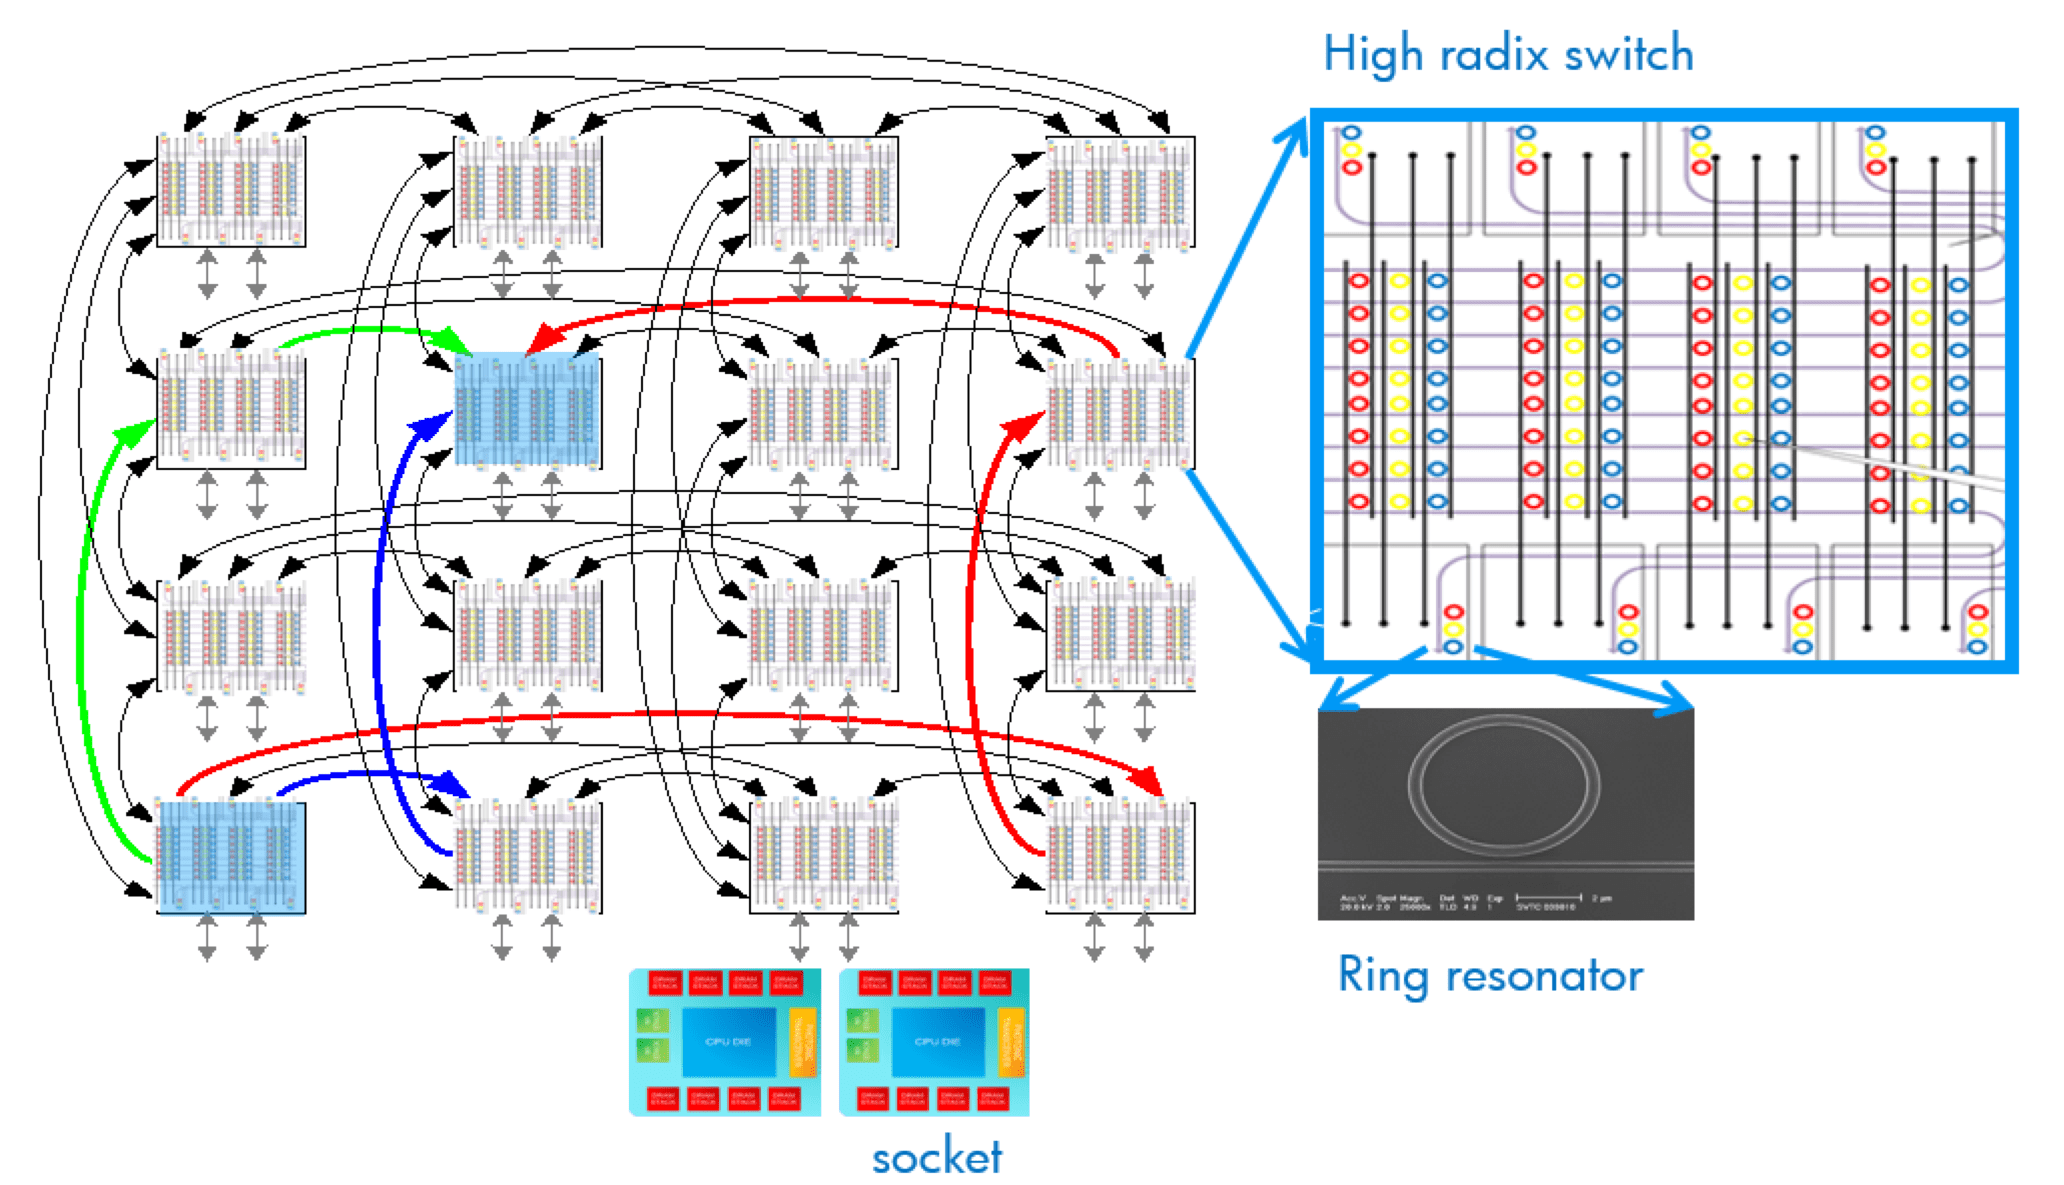
\includegraphics[width=14cm]{images/edl_photo_hyperX.png}
            \caption{\label{fig:edl_photo_hyperX} Topologie HyperX.}
        \end{figure} 
            
            %Module mémoire
                \begin{figure}
                \center
                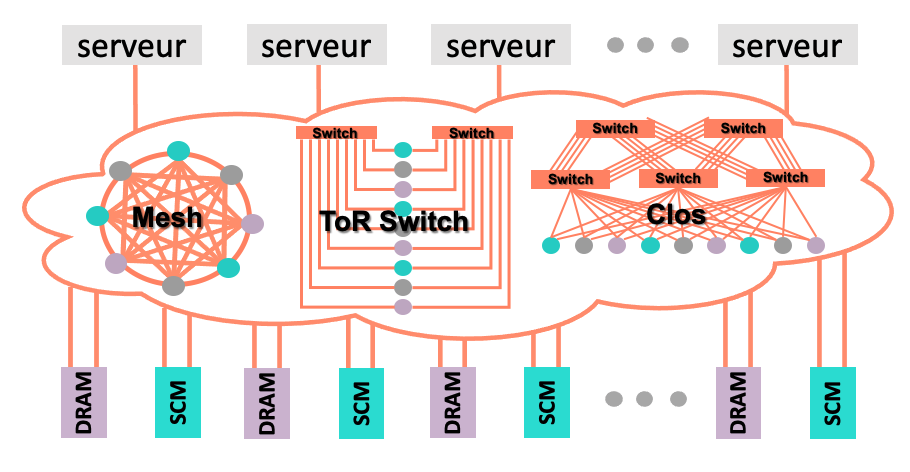
\includegraphics[width=14cm]{images/edl_genz_topo.png}
                \caption{\label{fig:edl_genz_topo} Le protocole Gen-Z permet d'implémenter nativement différentes topologies.}
            \end{figure}
            
            

    \paragraph{Sécurité}

        La sécurité est un aspect fondamental du développement de Gen-Z. La sécurisation des échanges est en effet très importante si ce protocole doit être utilisé à l'extérieur des centres de calculs. Chaque composant Gen-Z est identifié lors de leur création en usine. Il est ainsi possible d'authentifier n'importe quelle transaction. Le protocole peut ainsi permettre à un routeur de bloquer ou non une communication. La sécurité est réalisée par un logiciel centralisé et assuré physiquement par chaque matériel grâce à l’utilisation de clefs d’accès. Les accès interdits sont reportés au gestionnaire pour éventuellement déceler des attaques. De nombreux mécanismes de sécurité contre les attaques de type \textit{man-in-the-middle} comme l'utilisation de tags \textit{anti-replay} \cite{Radhakishan2011}.

    \subsubsection{Nouvelles plateformes} \label{sec:oppo_new_tech} \label{sec:compute_on_the_edge}
            
        Associé aux technologies présentées précédemment comme les mémoires non volatiles (SCM) et/ou les technologies d'interconnexion rapides à faible consommation (photoniques), Gen-Z va permettre de repenser l'architecture des plateformes. Le calcul piloté par la mémoire (Memory Driven Computing (architecture MDC)) désigne une nouvelle façon d'organiser les architectures en plaçant la mémoire au centre (voir \autoref{fig:edl_mdc}). L'architecture MDC donne à chaque processeur l'accès à un grand espace de mémoire partagée (\textit{memory pool}) (\autoref{fig:edl_mdc_new}). C'est la différence majeure avec les architectures actuelles où chaque processeur possède son propre espace mémoire local (\autoref{fig:edl_mdc_old}). L'avantage de cette architecture est de pouvoir combiner différents éléments de calcul (processeur, accélérateurs) autour de ces espaces mémoire. En fonction des besoins des applications, différentes plateformes peuvent être développées pour répondre précisément au besoin.
    
            \begin{figure}[t!]
                \centering
                \begin{subfigure}[t]{0.49\textwidth}
                    \centering
                    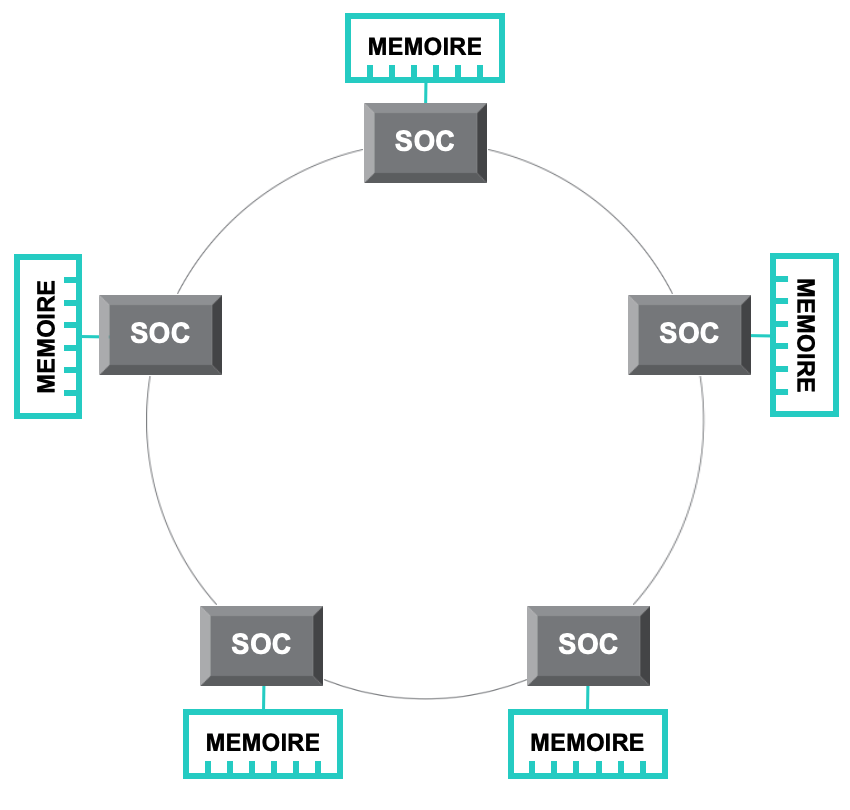
\includegraphics[width=\linewidth]{images/edl_mdc_old.png}
                    \caption{\label{fig:edl_mdc_old} Plateformes actuelles}
                \end{subfigure}\hfill
                \begin{subfigure}[t]{0.49\textwidth}
                    \centering
                    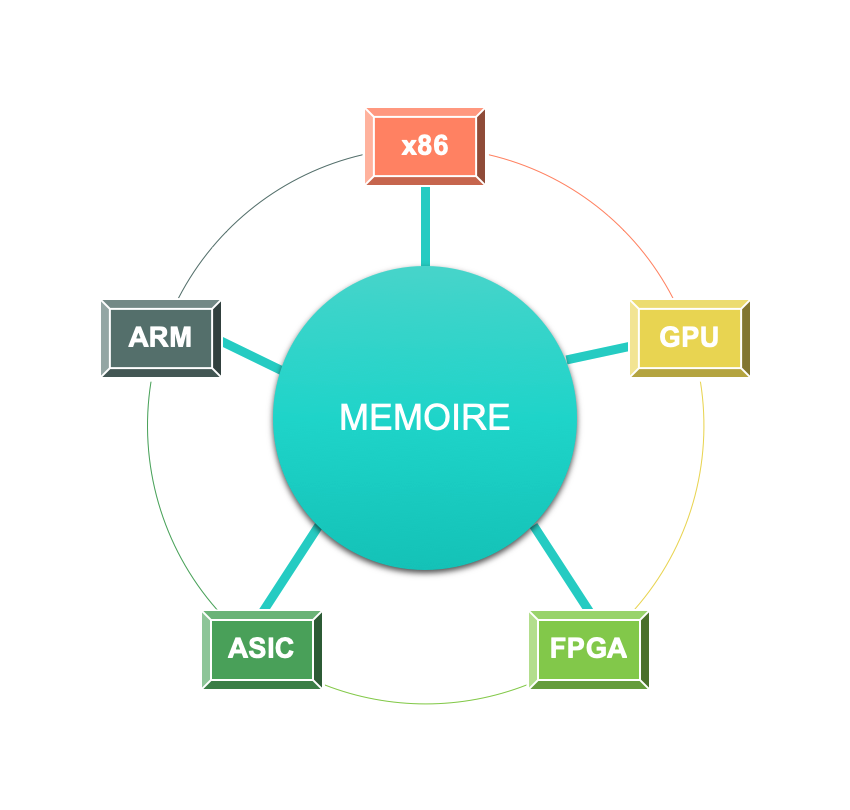
\includegraphics[width=\linewidth]{images/edl_mdc_new.png}
                    \caption{\label{fig:edl_mdc_new}Plateforme MDC}
                \end{subfigure}
                \caption{\label{fig:edl_mdc} Les plateformes MDC inversent l'architecture en plaçant la mémoire au centre.}
            \end{figure}

        %MEMORY
        Les trois principales caractéristiques dont vont bénéficier les applications sont: le \textit{partage} d'un \textit{grand espace} de mémoire \textit{persistant}. 
        Tous les serveurs \textbf{partageant} le même espace mémoire, il n'est plus nécessaire de réaliser des communications explicites pour échanger des données. Pour le programmeur, cela implique de ne plus avoir à se soucier de partitionner et répartir les jeux de données entre chaque serveur. 
        L'utilisation de \textbf{grands espaces mémoire} permet de repenser certains algorithmes. Par exemple en précalculant des graphes pour optimiser leur parcours, ou explorer simultanément plusieurs alternatives. En fonction des motifs d'accès mémoires réalisés, plusieurs versions d'un même jeu de données peuvent être utilisées permettant de profiter des techniques de localités.
        La totalité des jeux de données pouvant être stockée en \textbf{mémoires persistantes}, il n'est plus nécessaire de réaliser des sauvegardes régulières des données sur des périphériques de stockage beaucoup plus lents.

        %MEMORY POOL
        Un même module mémoire pourra être fragmenté et utilisé par différentes ressources. Grâce à Gen-Z, il est possible d'assigner dynamiquement une zone mémoire à une ressource même si celle-ci ne se trouve pas sur le même serveur.  Associés à des technologies comme la photonique, ces mémoires peuvent être accédées très rapidement permettant de créer des espaces mémoire distants de grande capacité. Une zone mémoire peut alors être partagée entre différentes ressources travaillant sur un même jeu de données, ou pour réaliser des communications en mémoire (synchronisation). Lorsqu'un accélérateur doit communiquer des résultats à un second accélérateur, il n'a qu'à lui autoriser l'accès à cette zone mémoire et lui transmettre un pointeur associé.
           
         %Superdome
         HPE développe depuis plusieurs années une architecture MDC connue sous le nom de code de \textit{The Machine}. Ce projet a donné lieu à la première gamme de serveurs MDC: HPE Superdome Flex. Ces plateformes peuvent embarquer 32 processeurs partageant 48 TB de mémoire. Les premiers résultats ont montré l'énorme saut de performance pouvant être atteint pour certaines applications. Une application de calcul de graphe \cite{Chen2016a} a ainsi pu être accélérée par un facteur 128 en utilisant une plateforme de 12 TB de mémoire. HPE utilise des simulateurs permettant de prédire les gains de performances qu'un algorithme peut potentiellement atteindre. Les résultats de ces simulations ont montré que certaines applications utilisées dans le domaine de la finance (simulation Monte-Carlo) pourraient être accélérées par un facteur 10000.
   
               
      \begin{figure}
        \center
        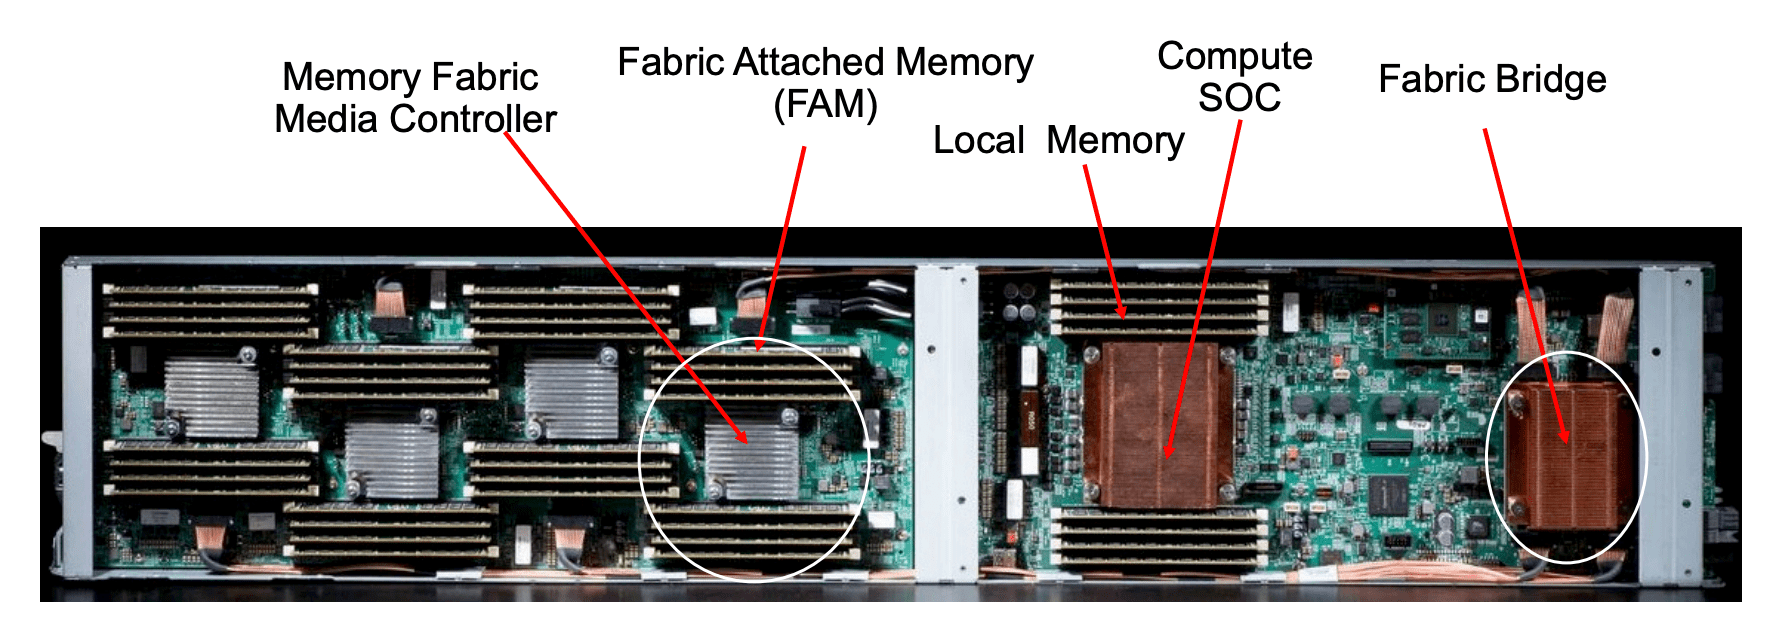
\includegraphics[width=14cm]{images/edl_superdome.png}
        \caption{\label{fig:edl_superdome}Les serveurs HPE Superdome possèdent un espace mémoire \textit{attaché} partagé entre les différents processeurs.}
        \end{figure}
